\documentclass[a4paper]{book}
\usepackage{makeidx}
\usepackage{graphicx}
\usepackage{multicol}
\usepackage{float}
\usepackage{listings}
\usepackage{color}
\usepackage{ifthen}
\usepackage[table]{xcolor}
\usepackage{textcomp}
\usepackage{alltt}
\usepackage[utf8]{inputenc}
\usepackage{mathptmx}
\usepackage[scaled=.90]{helvet}
\usepackage{courier}
\usepackage{doxygen}
\lstset{language=C++,inputencoding=utf8,basicstyle=\footnotesize,breaklines=true,breakatwhitespace=true,tabsize=8,numbers=left }
\makeindex
\setcounter{tocdepth}{3}
\renewcommand{\footrulewidth}{0.4pt}
\begin{document}
\begin{titlepage}
\vspace*{7cm}
\begin{center}
{\Large EMI File Transfer Service (FTS 3) \\[1ex]\large 0.0.0 }\\
\vspace*{1cm}
{\large Generated by Doxygen 1.7.3}\\
\vspace*{0.5cm}
{\small Wed Feb 8 2012 12:49:02}\\
\end{center}
\end{titlepage}
\clearemptydoublepage
\pagenumbering{roman}
\tableofcontents
\clearemptydoublepage
\pagenumbering{arabic}
\chapter{Service Definitions}
\label{index}Element \char`\"{}http://transfer.data.glite.org\char`\"{}:TransferExceptionElement of type \char`\"{}http://transfer.data.glite.org\char`\"{}:TransferException. Note: use wsdl2h option -\/g to generate this global element declaration. Element \char`\"{}http://transfer.data.glite.org\char`\"{}:InvalidArgumentExceptionElement of type \char`\"{}http://transfer.data.glite.org\char`\"{}:InvalidArgumentException. Note: use wsdl2h option -\/g to generate this global element declaration. Element \char`\"{}http://transfer.data.glite.org\char`\"{}:AuthorizationExceptionElement of type \char`\"{}http://transfer.data.glite.org\char`\"{}:AuthorizationException. Note: use wsdl2h option -\/g to generate this global element declaration. Element \char`\"{}http://transfer.data.glite.org\char`\"{}:ServiceBusyExceptionElement of type \char`\"{}http://transfer.data.glite.org\char`\"{}:ServiceBusyException. Note: use wsdl2h option -\/g to generate this global element declaration. Element \char`\"{}http://transfer.data.glite.org\char`\"{}:InternalExceptionElement of type \char`\"{}http://transfer.data.glite.org\char`\"{}:InternalException. Note: use wsdl2h option -\/g to generate this global element declaration. Element \char`\"{}http://transfer.data.glite.org\char`\"{}:NotExistsExceptionElement of type \char`\"{}http://transfer.data.glite.org\char`\"{}:NotExistsException. Note: use wsdl2h option -\/g to generate this global element declaration. Element \char`\"{}http://transfer.data.glite.org\char`\"{}:CannotCancelExceptionElement of type \char`\"{}http://transfer.data.glite.org\char`\"{}:CannotCancelException. Note: use wsdl2h option -\/g to generate this global element declaration. Element \char`\"{}http://transfer.data.glite.org\char`\"{}:ExistsExceptionElement of type \char`\"{}http://transfer.data.glite.org\char`\"{}:ExistsException. Note: use wsdl2h option -\/g to generate this global element declaration.\section{Bindings}\label{index_Service_bindings}

\begin{DoxyItemize}
\item \doxyref{Binding \char`\"{}FileTransferSoapBinding\char`\"{}}{p.}{FileTransferSoapBinding} 
\end{DoxyItemize}
\chapter{Binding \char`\"{}FileTransferSoapBinding\char`\"{}}
\label{FileTransferSoapBinding}
\section{Operations of Binding  \char`\"{}FileTransferSoapBinding\char`\"{}}\label{FileTransferSoapBinding_FileTransferSoapBinding_operations}

\begin{DoxyItemize}
\item \doxyref{fts\_\-\_\-placementSubmit}{p.}{structfts____placementSubmit}
\item \doxyref{fts\_\-\_\-placementSubmit2}{p.}{structfts____placementSubmit2}
\item \doxyref{fts\_\-\_\-transferSubmit}{p.}{structfts____transferSubmit}
\item \doxyref{fts\_\-\_\-transferSubmit2}{p.}{structfts____transferSubmit2}
\item \doxyref{fts\_\-\_\-transferSubmit3}{p.}{structfts____transferSubmit3}
\item \doxyref{fts\_\-\_\-submit}{p.}{structfts____submit}
\item \doxyref{fts\_\-\_\-listRequests}{p.}{structfts____listRequests}
\item \doxyref{fts\_\-\_\-listRequests2}{p.}{structfts____listRequests2}
\item \doxyref{fts\_\-\_\-getFileStatus}{p.}{structfts____getFileStatus}
\item \doxyref{fts\_\-\_\-getFileStatus2}{p.}{structfts____getFileStatus2}
\item \doxyref{fts\_\-\_\-getTransferJobStatus}{p.}{structfts____getTransferJobStatus}
\item \doxyref{fts\_\-\_\-getTransferJobSummary}{p.}{structfts____getTransferJobSummary}
\item \doxyref{fts\_\-\_\-getTransferJobSummary2}{p.}{structfts____getTransferJobSummary2}
\item \doxyref{fts\_\-\_\-cancel}{p.}{structfts____cancel}
\item \doxyref{fts\_\-\_\-setJobPriority}{p.}{structfts____setJobPriority}
\item \doxyref{fts\_\-\_\-addVOManager}{p.}{structfts____addVOManager}
\item \doxyref{fts\_\-\_\-removeVOManager}{p.}{structfts____removeVOManager}
\item \doxyref{fts\_\-\_\-listVOManagers}{p.}{structfts____listVOManagers}
\item \doxyref{fts\_\-\_\-getRoles}{p.}{structfts____getRoles}
\item \doxyref{fts\_\-\_\-getRolesOf}{p.}{structfts____getRolesOf}
\item \doxyref{fts\_\-\_\-getVersion}{p.}{structfts____getVersion}
\item \doxyref{fts\_\-\_\-getSchemaVersion}{p.}{structfts____getSchemaVersion}
\item \doxyref{fts\_\-\_\-getInterfaceVersion}{p.}{structfts____getInterfaceVersion}
\item \doxyref{fts\_\-\_\-getServiceMetadata}{p.}{structfts____getServiceMetadata}
\end{DoxyItemize}\section{Endpoints of Binding  \char`\"{}FileTransferSoapBinding\char`\"{}}\label{FileTransferSoapBinding_FileTransferSoapBinding_ports}

\begin{DoxyItemize}
\item {\tt https://localhost:8443/glite-\/data-\/transfer-\/interface/FileTransfer}
\end{DoxyItemize}

Note: use wsdl2h option -\/N to change the service binding prefix name 
\chapter{Data Structure Index}
\section{Class Hierarchy}
This inheritance list is sorted roughly, but not completely, alphabetically:\begin{DoxyCompactList}
\item \contentsline{section}{CliBase}{\pageref{classCliBase}}{}
\begin{DoxyCompactList}
\item \contentsline{section}{SubmitTransferCli}{\pageref{classSubmitTransferCli}}{}
\end{DoxyCompactList}
\item \contentsline{section}{CliManager}{\pageref{classCliManager}}{}
\item \contentsline{section}{FileTransferSoapBindingProxy}{\pageref{classFileTransferSoapBindingProxy}}{}
\item \contentsline{section}{fts\_\-\_\-addVOManager}{\pageref{structfts____addVOManager}}{}
\item \contentsline{section}{fts\_\-\_\-addVOManagerResponse}{\pageref{structfts____addVOManagerResponse}}{}
\item \contentsline{section}{fts\_\-\_\-ArrayOf\_\-USCOREsoapenc\_\-USCOREstring}{\pageref{classfts____ArrayOf__USCOREsoapenc__USCOREstring}}{}
\item \contentsline{section}{fts\_\-\_\-ArrayOf\_\-USCOREtns3\_\-USCOREFileTransferStatus}{\pageref{classfts____ArrayOf__USCOREtns3__USCOREFileTransferStatus}}{}
\item \contentsline{section}{fts\_\-\_\-ArrayOf\_\-USCOREtns3\_\-USCOREFileTransferStatus2}{\pageref{classfts____ArrayOf__USCOREtns3__USCOREFileTransferStatus2}}{}
\item \contentsline{section}{fts\_\-\_\-ArrayOf\_\-USCOREtns3\_\-USCOREJobStatus}{\pageref{classfts____ArrayOf__USCOREtns3__USCOREJobStatus}}{}
\item \contentsline{section}{fts\_\-\_\-cancel}{\pageref{structfts____cancel}}{}
\item \contentsline{section}{fts\_\-\_\-cancelResponse}{\pageref{structfts____cancelResponse}}{}
\item \contentsline{section}{fts\_\-\_\-getFileStatus}{\pageref{structfts____getFileStatus}}{}
\item \contentsline{section}{fts\_\-\_\-getFileStatus2}{\pageref{structfts____getFileStatus2}}{}
\item \contentsline{section}{fts\_\-\_\-getFileStatus2Response}{\pageref{structfts____getFileStatus2Response}}{}
\item \contentsline{section}{fts\_\-\_\-getFileStatusResponse}{\pageref{structfts____getFileStatusResponse}}{}
\item \contentsline{section}{fts\_\-\_\-getInterfaceVersion}{\pageref{structfts____getInterfaceVersion}}{}
\item \contentsline{section}{fts\_\-\_\-getInterfaceVersionResponse}{\pageref{structfts____getInterfaceVersionResponse}}{}
\item \contentsline{section}{fts\_\-\_\-getRoles}{\pageref{structfts____getRoles}}{}
\item \contentsline{section}{fts\_\-\_\-getRolesOf}{\pageref{structfts____getRolesOf}}{}
\item \contentsline{section}{fts\_\-\_\-getRolesOfResponse}{\pageref{structfts____getRolesOfResponse}}{}
\item \contentsline{section}{fts\_\-\_\-getRolesResponse}{\pageref{structfts____getRolesResponse}}{}
\item \contentsline{section}{fts\_\-\_\-getSchemaVersion}{\pageref{structfts____getSchemaVersion}}{}
\item \contentsline{section}{fts\_\-\_\-getSchemaVersionResponse}{\pageref{structfts____getSchemaVersionResponse}}{}
\item \contentsline{section}{fts\_\-\_\-getServiceMetadata}{\pageref{structfts____getServiceMetadata}}{}
\item \contentsline{section}{fts\_\-\_\-getServiceMetadataResponse}{\pageref{structfts____getServiceMetadataResponse}}{}
\item \contentsline{section}{fts\_\-\_\-getTransferJobStatus}{\pageref{structfts____getTransferJobStatus}}{}
\item \contentsline{section}{fts\_\-\_\-getTransferJobStatusResponse}{\pageref{structfts____getTransferJobStatusResponse}}{}
\item \contentsline{section}{fts\_\-\_\-getTransferJobSummary}{\pageref{structfts____getTransferJobSummary}}{}
\item \contentsline{section}{fts\_\-\_\-getTransferJobSummary2}{\pageref{structfts____getTransferJobSummary2}}{}
\item \contentsline{section}{fts\_\-\_\-getTransferJobSummary2Response}{\pageref{structfts____getTransferJobSummary2Response}}{}
\item \contentsline{section}{fts\_\-\_\-getTransferJobSummaryResponse}{\pageref{structfts____getTransferJobSummaryResponse}}{}
\item \contentsline{section}{fts\_\-\_\-getVersion}{\pageref{structfts____getVersion}}{}
\item \contentsline{section}{fts\_\-\_\-getVersionResponse}{\pageref{structfts____getVersionResponse}}{}
\item \contentsline{section}{fts\_\-\_\-listRequests}{\pageref{structfts____listRequests}}{}
\item \contentsline{section}{fts\_\-\_\-listRequests2}{\pageref{structfts____listRequests2}}{}
\item \contentsline{section}{fts\_\-\_\-listRequests2Response}{\pageref{structfts____listRequests2Response}}{}
\item \contentsline{section}{fts\_\-\_\-listRequestsResponse}{\pageref{structfts____listRequestsResponse}}{}
\item \contentsline{section}{fts\_\-\_\-listVOManagers}{\pageref{structfts____listVOManagers}}{}
\item \contentsline{section}{fts\_\-\_\-listVOManagersResponse}{\pageref{structfts____listVOManagersResponse}}{}
\item \contentsline{section}{fts\_\-\_\-placementSubmit}{\pageref{structfts____placementSubmit}}{}
\item \contentsline{section}{fts\_\-\_\-placementSubmit2}{\pageref{structfts____placementSubmit2}}{}
\item \contentsline{section}{fts\_\-\_\-placementSubmit2Response}{\pageref{structfts____placementSubmit2Response}}{}
\item \contentsline{section}{fts\_\-\_\-placementSubmitResponse}{\pageref{structfts____placementSubmitResponse}}{}
\item \contentsline{section}{fts\_\-\_\-removeVOManager}{\pageref{structfts____removeVOManager}}{}
\item \contentsline{section}{fts\_\-\_\-removeVOManagerResponse}{\pageref{structfts____removeVOManagerResponse}}{}
\item \contentsline{section}{fts\_\-\_\-setJobPriority}{\pageref{structfts____setJobPriority}}{}
\item \contentsline{section}{fts\_\-\_\-setJobPriorityResponse}{\pageref{structfts____setJobPriorityResponse}}{}
\item \contentsline{section}{fts\_\-\_\-submit}{\pageref{structfts____submit}}{}
\item \contentsline{section}{fts\_\-\_\-submitResponse}{\pageref{structfts____submitResponse}}{}
\item \contentsline{section}{fts\_\-\_\-transferSubmit}{\pageref{structfts____transferSubmit}}{}
\item \contentsline{section}{fts\_\-\_\-transferSubmit2}{\pageref{structfts____transferSubmit2}}{}
\item \contentsline{section}{fts\_\-\_\-transferSubmit2Response}{\pageref{structfts____transferSubmit2Response}}{}
\item \contentsline{section}{fts\_\-\_\-transferSubmit3}{\pageref{structfts____transferSubmit3}}{}
\item \contentsline{section}{fts\_\-\_\-transferSubmit3Response}{\pageref{structfts____transferSubmit3Response}}{}
\item \contentsline{section}{fts\_\-\_\-transferSubmitResponse}{\pageref{structfts____transferSubmitResponse}}{}
\item \contentsline{section}{SOAP\_\-ENV\_\-\_\-Code}{\pageref{structSOAP__ENV____Code}}{}
\item \contentsline{section}{SOAP\_\-ENV\_\-\_\-Detail}{\pageref{structSOAP__ENV____Detail}}{}
\item \contentsline{section}{SOAP\_\-ENV\_\-\_\-Fault}{\pageref{structSOAP__ENV____Fault}}{}
\item \contentsline{section}{SOAP\_\-ENV\_\-\_\-Header}{\pageref{structSOAP__ENV____Header}}{}
\item \contentsline{section}{SOAP\_\-ENV\_\-\_\-Reason}{\pageref{structSOAP__ENV____Reason}}{}
\item \contentsline{section}{transfer\_\-\_\-FileTransferStatus}{\pageref{classtransfer____FileTransferStatus}}{}
\begin{DoxyCompactList}
\item \contentsline{section}{transfer\_\-\_\-FileTransferStatus2}{\pageref{classtransfer____FileTransferStatus2}}{}
\item \contentsline{section}{transfer\_\-\_\-FileTransferStatus2}{\pageref{classtransfer____FileTransferStatus2}}{}
\end{DoxyCompactList}
\item \contentsline{section}{transfer\_\-\_\-JobStatus}{\pageref{classtransfer____JobStatus}}{}
\item \contentsline{section}{transfer\_\-\_\-PlacementJob}{\pageref{classtransfer____PlacementJob}}{}
\item \contentsline{section}{transfer\_\-\_\-Roles}{\pageref{classtransfer____Roles}}{}
\item \contentsline{section}{transfer\_\-\_\-StringPair}{\pageref{classtransfer____StringPair}}{}
\item \contentsline{section}{transfer\_\-\_\-TransferException}{\pageref{classtransfer____TransferException}}{}
\begin{DoxyCompactList}
\item \contentsline{section}{transfer\_\-\_\-AuthorizationException}{\pageref{classtransfer____AuthorizationException}}{}
\item \contentsline{section}{transfer\_\-\_\-AuthorizationException}{\pageref{classtransfer____AuthorizationException}}{}
\item \contentsline{section}{transfer\_\-\_\-CannotCancelException}{\pageref{classtransfer____CannotCancelException}}{}
\item \contentsline{section}{transfer\_\-\_\-CannotCancelException}{\pageref{classtransfer____CannotCancelException}}{}
\item \contentsline{section}{transfer\_\-\_\-ExistsException}{\pageref{classtransfer____ExistsException}}{}
\item \contentsline{section}{transfer\_\-\_\-ExistsException}{\pageref{classtransfer____ExistsException}}{}
\item \contentsline{section}{transfer\_\-\_\-InternalException}{\pageref{classtransfer____InternalException}}{}
\item \contentsline{section}{transfer\_\-\_\-InternalException}{\pageref{classtransfer____InternalException}}{}
\item \contentsline{section}{transfer\_\-\_\-InvalidArgumentException}{\pageref{classtransfer____InvalidArgumentException}}{}
\item \contentsline{section}{transfer\_\-\_\-InvalidArgumentException}{\pageref{classtransfer____InvalidArgumentException}}{}
\item \contentsline{section}{transfer\_\-\_\-NotExistsException}{\pageref{classtransfer____NotExistsException}}{}
\item \contentsline{section}{transfer\_\-\_\-NotExistsException}{\pageref{classtransfer____NotExistsException}}{}
\item \contentsline{section}{transfer\_\-\_\-ServiceBusyException}{\pageref{classtransfer____ServiceBusyException}}{}
\item \contentsline{section}{transfer\_\-\_\-ServiceBusyException}{\pageref{classtransfer____ServiceBusyException}}{}
\end{DoxyCompactList}
\item \contentsline{section}{transfer\_\-\_\-TransferJob}{\pageref{classtransfer____TransferJob}}{}
\item \contentsline{section}{transfer\_\-\_\-TransferJob2}{\pageref{classtransfer____TransferJob2}}{}
\item \contentsline{section}{transfer\_\-\_\-TransferJobElement}{\pageref{classtransfer____TransferJobElement}}{}
\item \contentsline{section}{transfer\_\-\_\-TransferJobElement2}{\pageref{classtransfer____TransferJobElement2}}{}
\item \contentsline{section}{transfer\_\-\_\-TransferJobSummary}{\pageref{classtransfer____TransferJobSummary}}{}
\begin{DoxyCompactList}
\item \contentsline{section}{transfer\_\-\_\-TransferJobSummary2}{\pageref{classtransfer____TransferJobSummary2}}{}
\item \contentsline{section}{transfer\_\-\_\-TransferJobSummary2}{\pageref{classtransfer____TransferJobSummary2}}{}
\end{DoxyCompactList}
\item \contentsline{section}{transfer\_\-\_\-TransferParams}{\pageref{classtransfer____TransferParams}}{}
\end{DoxyCompactList}

\chapter{Data Structure Index}
\section{Data Structures}
Here are the data structures with brief descriptions:\begin{DoxyCompactList}
\item\contentsline{section}{{\bf CliBase} }{\pageref{classCliBase}}{}
\item\contentsline{section}{{\bf CliManager} }{\pageref{classCliManager}}{}
\item\contentsline{section}{{\bf FileTransferSoapBindingProxy} }{\pageref{classFileTransferSoapBindingProxy}}{}
\item\contentsline{section}{{\bf fts\_\-\_\-addVOManager} }{\pageref{structfts____addVOManager}}{}
\item\contentsline{section}{{\bf fts\_\-\_\-addVOManagerResponse} (Operation response struct \char`\"{}fts\_\-\_\-addVOManagerResponse\char`\"{} of service binding \char`\"{}FileTransferSoapBinding\char`\"{} operation \char`\"{}fts\_\-\_\-addVOManager\char`\"{} )}{\pageref{structfts____addVOManagerResponse}}{}
\item\contentsline{section}{{\bf fts\_\-\_\-ArrayOf\_\-USCOREsoapenc\_\-USCOREstring} (\char`\"{}http://glite.org/wsdl/services/org.glite.data.transfer.fts\char`\"{}:ArrayOf\_\-soapenc\_\-string is a complexType )}{\pageref{classfts____ArrayOf__USCOREsoapenc__USCOREstring}}{}
\item\contentsline{section}{{\bf fts\_\-\_\-ArrayOf\_\-USCOREtns3\_\-USCOREFileTransferStatus} (\char`\"{}http://glite.org/wsdl/services/org.glite.data.transfer.fts\char`\"{}:ArrayOf\_\-tns3\_\-FileTransferStatus is a complexType )}{\pageref{classfts____ArrayOf__USCOREtns3__USCOREFileTransferStatus}}{}
\item\contentsline{section}{{\bf fts\_\-\_\-ArrayOf\_\-USCOREtns3\_\-USCOREFileTransferStatus2} (\char`\"{}http://glite.org/wsdl/services/org.glite.data.transfer.fts\char`\"{}:ArrayOf\_\-tns3\_\-FileTransferStatus2 is a complexType )}{\pageref{classfts____ArrayOf__USCOREtns3__USCOREFileTransferStatus2}}{}
\item\contentsline{section}{{\bf fts\_\-\_\-ArrayOf\_\-USCOREtns3\_\-USCOREJobStatus} (\char`\"{}http://glite.org/wsdl/services/org.glite.data.transfer.fts\char`\"{}:ArrayOf\_\-tns3\_\-JobStatus is a complexType )}{\pageref{classfts____ArrayOf__USCOREtns3__USCOREJobStatus}}{}
\item\contentsline{section}{{\bf fts\_\-\_\-cancel} }{\pageref{structfts____cancel}}{}
\item\contentsline{section}{{\bf fts\_\-\_\-cancelResponse} (Operation response struct \char`\"{}fts\_\-\_\-cancelResponse\char`\"{} of service binding \char`\"{}FileTransferSoapBinding\char`\"{} operation \char`\"{}fts\_\-\_\-cancel\char`\"{} )}{\pageref{structfts____cancelResponse}}{}
\item\contentsline{section}{{\bf fts\_\-\_\-getFileStatus} }{\pageref{structfts____getFileStatus}}{}
\item\contentsline{section}{{\bf fts\_\-\_\-getFileStatus2} }{\pageref{structfts____getFileStatus2}}{}
\item\contentsline{section}{{\bf fts\_\-\_\-getFileStatus2Response} (Operation response struct \char`\"{}fts\_\-\_\-getFileStatus2Response\char`\"{} of service binding \char`\"{}FileTransferSoapBinding\char`\"{} operation \char`\"{}fts\_\-\_\-getFileStatus2\char`\"{} )}{\pageref{structfts____getFileStatus2Response}}{}
\item\contentsline{section}{{\bf fts\_\-\_\-getFileStatusResponse} (Operation response struct \char`\"{}fts\_\-\_\-getFileStatusResponse\char`\"{} of service binding \char`\"{}FileTransferSoapBinding\char`\"{} operation \char`\"{}fts\_\-\_\-getFileStatus\char`\"{} )}{\pageref{structfts____getFileStatusResponse}}{}
\item\contentsline{section}{{\bf fts\_\-\_\-getInterfaceVersion} }{\pageref{structfts____getInterfaceVersion}}{}
\item\contentsline{section}{{\bf fts\_\-\_\-getInterfaceVersionResponse} (Operation response struct \char`\"{}fts\_\-\_\-getInterfaceVersionResponse\char`\"{} of service binding \char`\"{}FileTransferSoapBinding\char`\"{} operation \char`\"{}fts\_\-\_\-getInterfaceVersion\char`\"{} )}{\pageref{structfts____getInterfaceVersionResponse}}{}
\item\contentsline{section}{{\bf fts\_\-\_\-getRoles} }{\pageref{structfts____getRoles}}{}
\item\contentsline{section}{{\bf fts\_\-\_\-getRolesOf} }{\pageref{structfts____getRolesOf}}{}
\item\contentsline{section}{{\bf fts\_\-\_\-getRolesOfResponse} (Operation response struct \char`\"{}fts\_\-\_\-getRolesOfResponse\char`\"{} of service binding \char`\"{}FileTransferSoapBinding\char`\"{} operation \char`\"{}fts\_\-\_\-getRolesOf\char`\"{} )}{\pageref{structfts____getRolesOfResponse}}{}
\item\contentsline{section}{{\bf fts\_\-\_\-getRolesResponse} (Operation response struct \char`\"{}fts\_\-\_\-getRolesResponse\char`\"{} of service binding \char`\"{}FileTransferSoapBinding\char`\"{} operation \char`\"{}fts\_\-\_\-getRoles\char`\"{} )}{\pageref{structfts____getRolesResponse}}{}
\item\contentsline{section}{{\bf fts\_\-\_\-getSchemaVersion} }{\pageref{structfts____getSchemaVersion}}{}
\item\contentsline{section}{{\bf fts\_\-\_\-getSchemaVersionResponse} (Operation response struct \char`\"{}fts\_\-\_\-getSchemaVersionResponse\char`\"{} of service binding \char`\"{}FileTransferSoapBinding\char`\"{} operation \char`\"{}fts\_\-\_\-getSchemaVersion\char`\"{} )}{\pageref{structfts____getSchemaVersionResponse}}{}
\item\contentsline{section}{{\bf fts\_\-\_\-getServiceMetadata} }{\pageref{structfts____getServiceMetadata}}{}
\item\contentsline{section}{{\bf fts\_\-\_\-getServiceMetadataResponse} (Operation response struct \char`\"{}fts\_\-\_\-getServiceMetadataResponse\char`\"{} of service binding \char`\"{}FileTransferSoapBinding\char`\"{} operation \char`\"{}fts\_\-\_\-getServiceMetadata\char`\"{} )}{\pageref{structfts____getServiceMetadataResponse}}{}
\item\contentsline{section}{{\bf fts\_\-\_\-getTransferJobStatus} }{\pageref{structfts____getTransferJobStatus}}{}
\item\contentsline{section}{{\bf fts\_\-\_\-getTransferJobStatusResponse} (Operation response struct \char`\"{}fts\_\-\_\-getTransferJobStatusResponse\char`\"{} of service binding \char`\"{}FileTransferSoapBinding\char`\"{} operation \char`\"{}fts\_\-\_\-getTransferJobStatus\char`\"{} )}{\pageref{structfts____getTransferJobStatusResponse}}{}
\item\contentsline{section}{{\bf fts\_\-\_\-getTransferJobSummary} }{\pageref{structfts____getTransferJobSummary}}{}
\item\contentsline{section}{{\bf fts\_\-\_\-getTransferJobSummary2} }{\pageref{structfts____getTransferJobSummary2}}{}
\item\contentsline{section}{{\bf fts\_\-\_\-getTransferJobSummary2Response} (Operation response struct \char`\"{}fts\_\-\_\-getTransferJobSummary2Response\char`\"{} of service binding \char`\"{}FileTransferSoapBinding\char`\"{} operation \char`\"{}fts\_\-\_\-getTransferJobSummary2\char`\"{} )}{\pageref{structfts____getTransferJobSummary2Response}}{}
\item\contentsline{section}{{\bf fts\_\-\_\-getTransferJobSummaryResponse} (Operation response struct \char`\"{}fts\_\-\_\-getTransferJobSummaryResponse\char`\"{} of service binding \char`\"{}FileTransferSoapBinding\char`\"{} operation \char`\"{}fts\_\-\_\-getTransferJobSummary\char`\"{} )}{\pageref{structfts____getTransferJobSummaryResponse}}{}
\item\contentsline{section}{{\bf fts\_\-\_\-getVersion} }{\pageref{structfts____getVersion}}{}
\item\contentsline{section}{{\bf fts\_\-\_\-getVersionResponse} (Operation response struct \char`\"{}fts\_\-\_\-getVersionResponse\char`\"{} of service binding \char`\"{}FileTransferSoapBinding\char`\"{} operation \char`\"{}fts\_\-\_\-getVersion\char`\"{} )}{\pageref{structfts____getVersionResponse}}{}
\item\contentsline{section}{{\bf fts\_\-\_\-listRequests} }{\pageref{structfts____listRequests}}{}
\item\contentsline{section}{{\bf fts\_\-\_\-listRequests2} }{\pageref{structfts____listRequests2}}{}
\item\contentsline{section}{{\bf fts\_\-\_\-listRequests2Response} (Operation response struct \char`\"{}fts\_\-\_\-listRequests2Response\char`\"{} of service binding \char`\"{}FileTransferSoapBinding\char`\"{} operation \char`\"{}fts\_\-\_\-listRequests2\char`\"{} )}{\pageref{structfts____listRequests2Response}}{}
\item\contentsline{section}{{\bf fts\_\-\_\-listRequestsResponse} (Operation response struct \char`\"{}fts\_\-\_\-listRequestsResponse\char`\"{} of service binding \char`\"{}FileTransferSoapBinding\char`\"{} operation \char`\"{}fts\_\-\_\-listRequests\char`\"{} )}{\pageref{structfts____listRequestsResponse}}{}
\item\contentsline{section}{{\bf fts\_\-\_\-listVOManagers} }{\pageref{structfts____listVOManagers}}{}
\item\contentsline{section}{{\bf fts\_\-\_\-listVOManagersResponse} (Operation response struct \char`\"{}fts\_\-\_\-listVOManagersResponse\char`\"{} of service binding \char`\"{}FileTransferSoapBinding\char`\"{} operation \char`\"{}fts\_\-\_\-listVOManagers\char`\"{} )}{\pageref{structfts____listVOManagersResponse}}{}
\item\contentsline{section}{{\bf fts\_\-\_\-placementSubmit} }{\pageref{structfts____placementSubmit}}{}
\item\contentsline{section}{{\bf fts\_\-\_\-placementSubmit2} }{\pageref{structfts____placementSubmit2}}{}
\item\contentsline{section}{{\bf fts\_\-\_\-placementSubmit2Response} (Operation response struct \char`\"{}fts\_\-\_\-placementSubmit2Response\char`\"{} of service binding \char`\"{}FileTransferSoapBinding\char`\"{} operation \char`\"{}fts\_\-\_\-placementSubmit2\char`\"{} )}{\pageref{structfts____placementSubmit2Response}}{}
\item\contentsline{section}{{\bf fts\_\-\_\-placementSubmitResponse} (Operation response struct \char`\"{}fts\_\-\_\-placementSubmitResponse\char`\"{} of service binding \char`\"{}FileTransferSoapBinding\char`\"{} operation \char`\"{}fts\_\-\_\-placementSubmit\char`\"{} )}{\pageref{structfts____placementSubmitResponse}}{}
\item\contentsline{section}{{\bf fts\_\-\_\-removeVOManager} }{\pageref{structfts____removeVOManager}}{}
\item\contentsline{section}{{\bf fts\_\-\_\-removeVOManagerResponse} (Operation response struct \char`\"{}fts\_\-\_\-removeVOManagerResponse\char`\"{} of service binding \char`\"{}FileTransferSoapBinding\char`\"{} operation \char`\"{}fts\_\-\_\-removeVOManager\char`\"{} )}{\pageref{structfts____removeVOManagerResponse}}{}
\item\contentsline{section}{{\bf fts\_\-\_\-setJobPriority} }{\pageref{structfts____setJobPriority}}{}
\item\contentsline{section}{{\bf fts\_\-\_\-setJobPriorityResponse} (Operation response struct \char`\"{}fts\_\-\_\-setJobPriorityResponse\char`\"{} of service binding \char`\"{}FileTransferSoapBinding\char`\"{} operation \char`\"{}fts\_\-\_\-setJobPriority\char`\"{} )}{\pageref{structfts____setJobPriorityResponse}}{}
\item\contentsline{section}{{\bf fts\_\-\_\-submit} }{\pageref{structfts____submit}}{}
\item\contentsline{section}{{\bf fts\_\-\_\-submitResponse} (Operation response struct \char`\"{}fts\_\-\_\-submitResponse\char`\"{} of service binding \char`\"{}FileTransferSoapBinding\char`\"{} operation \char`\"{}fts\_\-\_\-submit\char`\"{} )}{\pageref{structfts____submitResponse}}{}
\item\contentsline{section}{{\bf fts\_\-\_\-transferSubmit} }{\pageref{structfts____transferSubmit}}{}
\item\contentsline{section}{{\bf fts\_\-\_\-transferSubmit2} }{\pageref{structfts____transferSubmit2}}{}
\item\contentsline{section}{{\bf fts\_\-\_\-transferSubmit2Response} (Operation response struct \char`\"{}fts\_\-\_\-transferSubmit2Response\char`\"{} of service binding \char`\"{}FileTransferSoapBinding\char`\"{} operation \char`\"{}fts\_\-\_\-transferSubmit2\char`\"{} )}{\pageref{structfts____transferSubmit2Response}}{}
\item\contentsline{section}{{\bf fts\_\-\_\-transferSubmit3} }{\pageref{structfts____transferSubmit3}}{}
\item\contentsline{section}{{\bf fts\_\-\_\-transferSubmit3Response} (Operation response struct \char`\"{}fts\_\-\_\-transferSubmit3Response\char`\"{} of service binding \char`\"{}FileTransferSoapBinding\char`\"{} operation \char`\"{}fts\_\-\_\-transferSubmit3\char`\"{} )}{\pageref{structfts____transferSubmit3Response}}{}
\item\contentsline{section}{{\bf fts\_\-\_\-transferSubmitResponse} (Operation response struct \char`\"{}fts\_\-\_\-transferSubmitResponse\char`\"{} of service binding \char`\"{}FileTransferSoapBinding\char`\"{} operation \char`\"{}fts\_\-\_\-transferSubmit\char`\"{} )}{\pageref{structfts____transferSubmitResponse}}{}
\item\contentsline{section}{{\bf SOAP\_\-ENV\_\-\_\-Code} }{\pageref{structSOAP__ENV____Code}}{}
\item\contentsline{section}{{\bf SOAP\_\-ENV\_\-\_\-Detail} }{\pageref{structSOAP__ENV____Detail}}{}
\item\contentsline{section}{{\bf SOAP\_\-ENV\_\-\_\-Fault} }{\pageref{structSOAP__ENV____Fault}}{}
\item\contentsline{section}{{\bf SOAP\_\-ENV\_\-\_\-Header} }{\pageref{structSOAP__ENV____Header}}{}
\item\contentsline{section}{{\bf SOAP\_\-ENV\_\-\_\-Reason} }{\pageref{structSOAP__ENV____Reason}}{}
\item\contentsline{section}{{\bf SubmitTransferCli} }{\pageref{classSubmitTransferCli}}{}
\item\contentsline{section}{{\bf transfer\_\-\_\-AuthorizationException} (\char`\"{}http://transfer.data.glite.org\char`\"{}:AuthorizationException is a complexType with complexContent extension of \char`\"{}http://transfer.data.glite.org\char`\"{}:TransferException )}{\pageref{classtransfer____AuthorizationException}}{}
\item\contentsline{section}{{\bf transfer\_\-\_\-CannotCancelException} (\char`\"{}http://transfer.data.glite.org\char`\"{}:CannotCancelException is a complexType with complexContent extension of \char`\"{}http://transfer.data.glite.org\char`\"{}:TransferException )}{\pageref{classtransfer____CannotCancelException}}{}
\item\contentsline{section}{{\bf transfer\_\-\_\-ExistsException} (\char`\"{}http://transfer.data.glite.org\char`\"{}:ExistsException is a complexType with complexContent extension of \char`\"{}http://transfer.data.glite.org\char`\"{}:TransferException )}{\pageref{classtransfer____ExistsException}}{}
\item\contentsline{section}{{\bf transfer\_\-\_\-FileTransferStatus} (\char`\"{}http://transfer.data.glite.org\char`\"{}:FileTransferStatus is a complexType )}{\pageref{classtransfer____FileTransferStatus}}{}
\item\contentsline{section}{{\bf transfer\_\-\_\-FileTransferStatus2} (\char`\"{}http://transfer.data.glite.org\char`\"{}:FileTransferStatus2 is a complexType with complexContent extension of \char`\"{}http://transfer.data.glite.org\char`\"{}:FileTransferStatus )}{\pageref{classtransfer____FileTransferStatus2}}{}
\item\contentsline{section}{{\bf transfer\_\-\_\-InternalException} (\char`\"{}http://transfer.data.glite.org\char`\"{}:InternalException is a complexType with complexContent extension of \char`\"{}http://transfer.data.glite.org\char`\"{}:TransferException )}{\pageref{classtransfer____InternalException}}{}
\item\contentsline{section}{{\bf transfer\_\-\_\-InvalidArgumentException} (\char`\"{}http://transfer.data.glite.org\char`\"{}:InvalidArgumentException is a complexType with complexContent extension of \char`\"{}http://transfer.data.glite.org\char`\"{}:TransferException )}{\pageref{classtransfer____InvalidArgumentException}}{}
\item\contentsline{section}{{\bf transfer\_\-\_\-JobStatus} (\char`\"{}http://transfer.data.glite.org\char`\"{}:JobStatus is a complexType )}{\pageref{classtransfer____JobStatus}}{}
\item\contentsline{section}{{\bf transfer\_\-\_\-NotExistsException} (\char`\"{}http://transfer.data.glite.org\char`\"{}:NotExistsException is a complexType with complexContent extension of \char`\"{}http://transfer.data.glite.org\char`\"{}:TransferException )}{\pageref{classtransfer____NotExistsException}}{}
\item\contentsline{section}{{\bf transfer\_\-\_\-PlacementJob} (\char`\"{}http://transfer.data.glite.org\char`\"{}:PlacementJob is a complexType )}{\pageref{classtransfer____PlacementJob}}{}
\item\contentsline{section}{{\bf transfer\_\-\_\-Roles} (\char`\"{}http://transfer.data.glite.org\char`\"{}:Roles is a complexType )}{\pageref{classtransfer____Roles}}{}
\item\contentsline{section}{{\bf transfer\_\-\_\-ServiceBusyException} (\char`\"{}http://transfer.data.glite.org\char`\"{}:ServiceBusyException is a complexType with complexContent extension of \char`\"{}http://transfer.data.glite.org\char`\"{}:TransferException )}{\pageref{classtransfer____ServiceBusyException}}{}
\item\contentsline{section}{{\bf transfer\_\-\_\-StringPair} (\char`\"{}http://transfer.data.glite.org\char`\"{}:StringPair is a complexType )}{\pageref{classtransfer____StringPair}}{}
\item\contentsline{section}{{\bf transfer\_\-\_\-TransferException} (\char`\"{}http://transfer.data.glite.org\char`\"{}:TransferException is a complexType )}{\pageref{classtransfer____TransferException}}{}
\item\contentsline{section}{{\bf transfer\_\-\_\-TransferJob} (\char`\"{}http://transfer.data.glite.org\char`\"{}:TransferJob is a complexType )}{\pageref{classtransfer____TransferJob}}{}
\item\contentsline{section}{{\bf transfer\_\-\_\-TransferJob2} (\char`\"{}http://transfer.data.glite.org\char`\"{}:TransferJob2 is a complexType )}{\pageref{classtransfer____TransferJob2}}{}
\item\contentsline{section}{{\bf transfer\_\-\_\-TransferJobElement} (\char`\"{}http://transfer.data.glite.org\char`\"{}:TransferJobElement is a complexType )}{\pageref{classtransfer____TransferJobElement}}{}
\item\contentsline{section}{{\bf transfer\_\-\_\-TransferJobElement2} (\char`\"{}http://transfer.data.glite.org\char`\"{}:TransferJobElement2 is a complexType )}{\pageref{classtransfer____TransferJobElement2}}{}
\item\contentsline{section}{{\bf transfer\_\-\_\-TransferJobSummary} (\char`\"{}http://transfer.data.glite.org\char`\"{}:TransferJobSummary is a complexType )}{\pageref{classtransfer____TransferJobSummary}}{}
\item\contentsline{section}{{\bf transfer\_\-\_\-TransferJobSummary2} (\char`\"{}http://transfer.data.glite.org\char`\"{}:TransferJobSummary2 is a complexType with complexContent extension of \char`\"{}http://transfer.data.glite.org\char`\"{}:TransferJobSummary )}{\pageref{classtransfer____TransferJobSummary2}}{}
\item\contentsline{section}{{\bf transfer\_\-\_\-TransferParams} (\char`\"{}http://transfer.data.glite.org\char`\"{}:TransferParams is a complexType )}{\pageref{classtransfer____TransferParams}}{}
\end{DoxyCompactList}

\chapter{Data Structure Documentation}
\section{CliBase Class Reference}
\label{classCliBase}\index{CliBase@{CliBase}}
Inheritance diagram for CliBase:\begin{figure}[H]
\begin{center}
\leavevmode
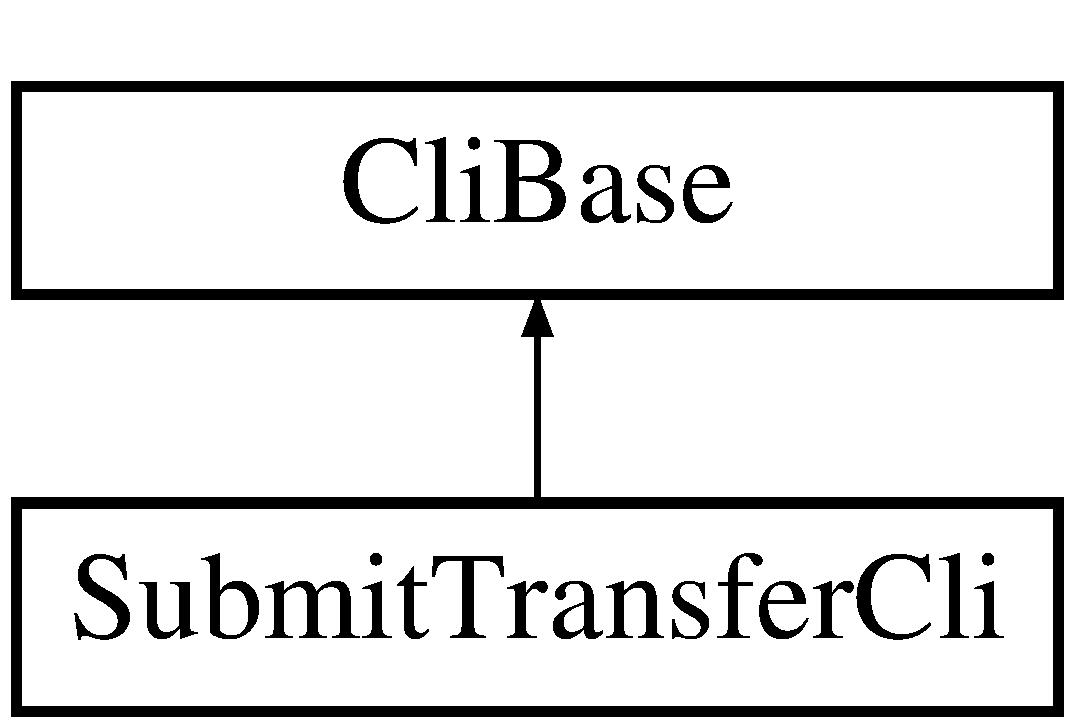
\includegraphics[height=2.000000cm]{classCliBase}
\end{center}
\end{figure}
\subsection*{Public Member Functions}
\begin{DoxyCompactItemize}
\item 
void {\bfseries initCli} (int ac, char $\ast$av[$\,$])\label{classCliBase_a4bd2ca28f56f6423d7d3f01c1749f0f5}

\item 
bool {\bfseries printHelp} ()\label{classCliBase_aa20d5af1689dbb8d5dc59cb050b2be6a}

\item 
bool {\bfseries printVersion} ()\label{classCliBase_a62246bf8d045ba1dcf9b2620fefe7a49}

\item 
bool {\bfseries isVerbose} ()\label{classCliBase_af5f028e631157613fee035627f753410}

\item 
bool {\bfseries isQuite} ()\label{classCliBase_a3f88608927308c1b0d7504b9ff126374}

\item 
string {\bfseries getService} ()\label{classCliBase_a98d6e23a92238d5b364abc488e2aca4f}

\item 
string {\bfseries getSource} ()\label{classCliBase_a5a35901fc89ccac29bc7ccd00b13ea15}

\item 
string {\bfseries getDestination} ()\label{classCliBase_ad73c2f9744627774b0d0dcc7f43780fb}

\end{DoxyCompactItemize}
\subsection*{Protected Member Functions}
\begin{DoxyCompactItemize}
\item 
string {\bfseries discoverService} ()\label{classCliBase_aba9d7a499eaf393077ba31bd133dafca}

\end{DoxyCompactItemize}
\subsection*{Protected Attributes}
\begin{DoxyCompactItemize}
\item 
variables\_\-map {\bfseries vm}\label{classCliBase_a6f1a8ef69828b6effbd13b8f3dffd488}

\item 
options\_\-description {\bfseries basic}\label{classCliBase_a8adc76a9f4d22fabc4423b4ca23f4230}

\item 
options\_\-description {\bfseries cli\_\-options}\label{classCliBase_a9ff6498292f4a734e7a58f45bf32f2f1}

\item 
positional\_\-options\_\-description {\bfseries p}\label{classCliBase_a54f228b90881646fb8cfedd8c94837ba}

\item 
string {\bfseries endpoint}\label{classCliBase_a3aa9c753bf08040299e01d32f7c7094c}

\end{DoxyCompactItemize}


\subsection{Detailed Description}


Definition at line 16 of file CliBase.h.



The documentation for this class was generated from the following files:\begin{DoxyCompactItemize}
\item 
src/CLI/CliBase.h\item 
src/CLI/CliBase.cpp\end{DoxyCompactItemize}

\section{CliManager Class Reference}
\label{classCliManager}\index{CliManager@{CliManager}}
\subsection*{Public Member Functions}
\begin{DoxyCompactItemize}
\item 
void {\bfseries setInterface} (string interface)\label{classCliManager_a608657d968ef29d26ca94b648ce31f21}

\item 
string {\bfseries getPassword} ()\label{classCliManager_a1120fd8ff83eced525df8c1d9b6f5808}

\item 
int {\bfseries isChecksumSupported} ()\label{classCliManager_a6a8aa8dd522167c43a869baf2c637ce4}

\item 
int {\bfseries isDelegationSupported} ()\label{classCliManager_a207cc6e6311fe97c9b9a2d1a068ae916}

\item 
int {\bfseries isRolesOfSupported} ()\label{classCliManager_ab6f5ece0cd572e80fc17abee344cd54e}

\item 
int {\bfseries isSetTCPBufferSupported} ()\label{classCliManager_a680689bce96ce643070b45c0fb909eec}

\item 
int {\bfseries isExtendedChannelListSupported} ()\label{classCliManager_a44116782069f1ab850b141f18be6b663}

\item 
int {\bfseries isChannelMessageSupported} ()\label{classCliManager_a2c8f5f265a9e59fc8c536de77a47794b}

\item 
int {\bfseries isUserVoRestrictListingSupported} ()\label{classCliManager_a79e6f679e6720ac08a6384cfbc5aaa94}

\item 
int {\bfseries isVersion330StatesSupported} ()\label{classCliManager_ab07e406b612ba34b3e0cb473427395e5}

\item 
int {\bfseries isItVersion330} ()\label{classCliManager_a52b71857143a64320b869225aad3402f}

\item 
int {\bfseries isItVersion340} ()\label{classCliManager_a6bee47c816344138811a7665054b8f60}

\item 
int {\bfseries isItVersion350} ()\label{classCliManager_a7f7fd2ff29c5a95b3ddb5c2dd2240d48}

\item 
int {\bfseries isItVersion370} ()\label{classCliManager_a2a2705c7296217728ab0c4c93151c972}

\end{DoxyCompactItemize}
\subsection*{Static Public Member Functions}
\begin{DoxyCompactItemize}
\item 
static {\bf CliManager} $\ast$ {\bfseries getInstance} ()\label{classCliManager_af57b7314f1b46545d3d07055a9a96578}

\end{DoxyCompactItemize}
\subsection*{Data Fields}
\begin{DoxyCompactItemize}
\item 
string {\bfseries FTS3\_\-PARAM\_\-GRIDFTP}\label{classCliManager_a6b85959ca6e7f83a2dc1080810f54742}

\item 
string {\bfseries FTS3\_\-PARAM\_\-MYPROXY}\label{classCliManager_a5138b724bb7cdad2ece461f461418d42}

\item 
string {\bfseries FTS3\_\-PARAM\_\-DELEGATIONID}\label{classCliManager_ab7bdb8836e0d3789f6acb1fd4f4d7eca}

\item 
string {\bfseries FTS3\_\-PARAM\_\-SPACETOKEN}\label{classCliManager_a0bb93b6fc6e7dbfa1219934d8ba37265}

\item 
string {\bfseries FTS3\_\-PARAM\_\-SPACETOKEN\_\-SOURCE}\label{classCliManager_a0a14ec3c952e0891b8a3351933b4d47e}

\item 
string {\bfseries FTS3\_\-PARAM\_\-COPY\_\-PIN\_\-LIFETIME}\label{classCliManager_a510a7710137bfa97a113b4684f266424}

\item 
string {\bfseries FTS3\_\-PARAM\_\-LAN\_\-CONNECTION}\label{classCliManager_a3e92365401259a3cc13268baee5eaffa}

\item 
string {\bfseries FTS3\_\-PARAM\_\-FAIL\_\-NEARLINE}\label{classCliManager_a5942426466438df29420acbfd6c48709}

\item 
string {\bfseries FTS3\_\-PARAM\_\-OVERWRITEFLAG}\label{classCliManager_a5648f2bf1d8746b8632d2b3072ba8c08}

\item 
string {\bfseries FTS3\_\-PARAM\_\-CHECKSUM\_\-METHOD}\label{classCliManager_a2708547972dcbcc46622b923543ba3f7}

\item 
string {\bfseries FTS3\_\-CA\_\-SD\_\-TYPE}\label{classCliManager_a34048663a89b917fa76f20bc2e283923}

\item 
string {\bfseries FTS3\_\-SD\_\-ENV}\label{classCliManager_a787d355931904bcedba4f0345ac1ec27}

\item 
string {\bfseries FTS3\_\-SD\_\-TYPE}\label{classCliManager_ade03c3d47c10811aaaa6e0368392fa80}

\item 
string {\bfseries FTS3\_\-IFC\_\-VERSION}\label{classCliManager_a83f99d6ccb12638730d9ee3d18e1edee}

\item 
string {\bfseries FTS3\_\-INTERFACE\_\-VERSION}\label{classCliManager_a10f9907c34a192bc8cc796de2d2d8591}

\end{DoxyCompactItemize}


\subsection{Detailed Description}


Definition at line 14 of file CliManager.h.



The documentation for this class was generated from the following files:\begin{DoxyCompactItemize}
\item 
src/CLI/CliManager.h\item 
src/CLI/CliManager.cpp\end{DoxyCompactItemize}

\section{FileTransferSoapBindingProxy Class Reference}
\label{classFileTransferSoapBindingProxy}\index{FileTransferSoapBindingProxy@{FileTransferSoapBindingProxy}}
\subsection*{Public Member Functions}
\begin{DoxyCompactItemize}
\item 
{\bf FileTransferSoapBindingProxy} ()\label{classFileTransferSoapBindingProxy_aca393829334a168ce236cba823fcc020}

\begin{DoxyCompactList}\small\item\em Constructor. \item\end{DoxyCompactList}\item 
{\bf FileTransferSoapBindingProxy} (const struct soap \&)\label{classFileTransferSoapBindingProxy_acd4c77d2cce6e66cd458895728b9614f}

\begin{DoxyCompactList}\small\item\em Constructor with copy of another engine state. \item\end{DoxyCompactList}\item 
{\bf FileTransferSoapBindingProxy} (soap\_\-mode iomode)\label{classFileTransferSoapBindingProxy_a2882dfc1cf48cf251227a5bd6331855c}

\begin{DoxyCompactList}\small\item\em Constructor with engine input+output mode control. \item\end{DoxyCompactList}\item 
{\bf FileTransferSoapBindingProxy} (soap\_\-mode imode, soap\_\-mode omode)\label{classFileTransferSoapBindingProxy_a28b0b3aebf1c1941913fd6f037967617}

\begin{DoxyCompactList}\small\item\em Constructor with engine input and output mode control. \item\end{DoxyCompactList}\item 
virtual {\bf $\sim$FileTransferSoapBindingProxy} ()\label{classFileTransferSoapBindingProxy_acd5dd13a11ceafa7b16971f45a1e0ac2}

\begin{DoxyCompactList}\small\item\em Destructor frees deserialized data. \item\end{DoxyCompactList}\item 
virtual void {\bf FileTransferSoapBindingProxy\_\-init} (soap\_\-mode imode, soap\_\-mode omode)\label{classFileTransferSoapBindingProxy_a19ad46adf3256c3bb390a7568aae9309}

\begin{DoxyCompactList}\small\item\em Initializer used by constructor. \item\end{DoxyCompactList}\item 
virtual void {\bf soap\_\-noheader} ()\label{classFileTransferSoapBindingProxy_aad8ec48d598fc29bfa4387187efc3da8}

\begin{DoxyCompactList}\small\item\em Disables and removes SOAP Header from message. \item\end{DoxyCompactList}\item 
virtual const {\bf SOAP\_\-ENV\_\-\_\-Fault} $\ast$ {\bf soap\_\-fault} ()\label{classFileTransferSoapBindingProxy_af29c64eae217e44a0c5ce1443ff15697}

\begin{DoxyCompactList}\small\item\em Get SOAP Fault structure (NULL when absent) \item\end{DoxyCompactList}\item 
virtual const char $\ast$ {\bf soap\_\-fault\_\-string} ()\label{classFileTransferSoapBindingProxy_a86c9e09a198d62eb5ead5a2a7c2b6967}

\begin{DoxyCompactList}\small\item\em Get SOAP Fault string (NULL when absent) \item\end{DoxyCompactList}\item 
virtual const char $\ast$ {\bf soap\_\-fault\_\-detail} ()\label{classFileTransferSoapBindingProxy_a0da5102ac7bd9cbcb06ed48b843b89d2}

\begin{DoxyCompactList}\small\item\em Get SOAP Fault detail as string (NULL when absent) \item\end{DoxyCompactList}\item 
virtual int {\bf soap\_\-close\_\-socket} ()\label{classFileTransferSoapBindingProxy_a8bd7fc4257c76c60fddf8729f51103a0}

\begin{DoxyCompactList}\small\item\em Force close connection (normally automatic, except for send\_\-X ops) \item\end{DoxyCompactList}\item 
virtual void {\bf soap\_\-print\_\-fault} (FILE $\ast$)\label{classFileTransferSoapBindingProxy_a32c3234408f0fae1558b3300979c2c22}

\begin{DoxyCompactList}\small\item\em Print fault. \item\end{DoxyCompactList}\item 
virtual void {\bf soap\_\-stream\_\-fault} (std::ostream \&)\label{classFileTransferSoapBindingProxy_a9777244fc33e12f1dadf6612d1104725}

\begin{DoxyCompactList}\small\item\em Print fault to stream. \item\end{DoxyCompactList}\item 
virtual char $\ast$ {\bf soap\_\-sprint\_\-fault} (char $\ast$buf, size\_\-t len)\label{classFileTransferSoapBindingProxy_ac1ceea6b8908256f729f36df2ce84cd8}

\begin{DoxyCompactList}\small\item\em Put fault into buffer. \item\end{DoxyCompactList}\item 
virtual int {\bf placementSubmit} ({\bf transfer\_\-\_\-PlacementJob} $\ast$\_\-job, struct {\bf fts\_\-\_\-placementSubmitResponse} \&\_\-param\_\-1)\label{classFileTransferSoapBindingProxy_a30cdbe874c532dbfb3cfdc9cef76b29f}

\begin{DoxyCompactList}\small\item\em Web service operation 'placementSubmit' (returns error code or SOAP\_\-OK) \item\end{DoxyCompactList}\item 
virtual int {\bf placementSubmit2} ({\bf transfer\_\-\_\-PlacementJob} $\ast$\_\-job, struct {\bf fts\_\-\_\-placementSubmit2Response} \&\_\-param\_\-2)\label{classFileTransferSoapBindingProxy_a95ae86beb66f856f1eeb560bb090c1e6}

\begin{DoxyCompactList}\small\item\em Web service operation 'placementSubmit2' (returns error code or SOAP\_\-OK) \item\end{DoxyCompactList}\item 
virtual int {\bf transferSubmit} ({\bf transfer\_\-\_\-TransferJob} $\ast$\_\-job, struct {\bf fts\_\-\_\-transferSubmitResponse} \&\_\-param\_\-3)\label{classFileTransferSoapBindingProxy_a4a5d6b9e5d79847a62765aa43badd170}

\begin{DoxyCompactList}\small\item\em Web service operation 'transferSubmit' (returns error code or SOAP\_\-OK) \item\end{DoxyCompactList}\item 
virtual int {\bf transferSubmit2} ({\bf transfer\_\-\_\-TransferJob} $\ast$\_\-job, struct {\bf fts\_\-\_\-transferSubmit2Response} \&\_\-param\_\-4)\label{classFileTransferSoapBindingProxy_a9ca95039536d47a3185623b91d1c46d9}

\begin{DoxyCompactList}\small\item\em Web service operation 'transferSubmit2' (returns error code or SOAP\_\-OK) \item\end{DoxyCompactList}\item 
virtual int {\bf transferSubmit3} ({\bf transfer\_\-\_\-TransferJob2} $\ast$\_\-job, struct {\bf fts\_\-\_\-transferSubmit3Response} \&\_\-param\_\-5)\label{classFileTransferSoapBindingProxy_abd61ae0a80ec18990c0e0cca97e87817}

\begin{DoxyCompactList}\small\item\em Web service operation 'transferSubmit3' (returns error code or SOAP\_\-OK) \item\end{DoxyCompactList}\item 
virtual int {\bf submit} ({\bf transfer\_\-\_\-TransferJob} $\ast$\_\-job, struct {\bf fts\_\-\_\-submitResponse} \&\_\-param\_\-6)\label{classFileTransferSoapBindingProxy_ad49e19443c157698ec08f89f8da9ed77}

\begin{DoxyCompactList}\small\item\em Web service operation 'submit' (returns error code or SOAP\_\-OK) \item\end{DoxyCompactList}\item 
virtual int {\bf listRequests} ({\bf fts\_\-\_\-ArrayOf\_\-USCOREsoapenc\_\-USCOREstring} $\ast$\_\-inGivenStates, struct {\bf fts\_\-\_\-listRequestsResponse} \&\_\-param\_\-7)\label{classFileTransferSoapBindingProxy_aa7ae039d5f382180dc9b0dcfb24c2828}

\begin{DoxyCompactList}\small\item\em Web service operation 'listRequests' (returns error code or SOAP\_\-OK) \item\end{DoxyCompactList}\item 
virtual int {\bf listRequests2} ({\bf fts\_\-\_\-ArrayOf\_\-USCOREsoapenc\_\-USCOREstring} $\ast$\_\-inGivenStates, std::string \_\-forDN, std::string \_\-forVO, struct {\bf fts\_\-\_\-listRequests2Response} \&\_\-param\_\-8)\label{classFileTransferSoapBindingProxy_a12e598eb0f9a15ca04e46c8f0ff69518}

\begin{DoxyCompactList}\small\item\em Web service operation 'listRequests2' (returns error code or SOAP\_\-OK) \item\end{DoxyCompactList}\item 
virtual int {\bf getFileStatus} (std::string \_\-requestID, int \_\-offset, int \_\-limit, struct {\bf fts\_\-\_\-getFileStatusResponse} \&\_\-param\_\-9)\label{classFileTransferSoapBindingProxy_ab374cacbbe79e006fd6781814e7bccee}

\begin{DoxyCompactList}\small\item\em Web service operation 'getFileStatus' (returns error code or SOAP\_\-OK) \item\end{DoxyCompactList}\item 
virtual int {\bf getFileStatus2} (std::string \_\-requestID, int \_\-offset, int \_\-limit, struct {\bf fts\_\-\_\-getFileStatus2Response} \&\_\-param\_\-10)\label{classFileTransferSoapBindingProxy_abdc6d108208bad5b1d8ea78f34499f5c}

\begin{DoxyCompactList}\small\item\em Web service operation 'getFileStatus2' (returns error code or SOAP\_\-OK) \item\end{DoxyCompactList}\item 
virtual int {\bf getTransferJobStatus} (std::string \_\-requestID, struct {\bf fts\_\-\_\-getTransferJobStatusResponse} \&\_\-param\_\-11)\label{classFileTransferSoapBindingProxy_a8db5bbfc833a80420e544f6d5dd6444a}

\begin{DoxyCompactList}\small\item\em Web service operation 'getTransferJobStatus' (returns error code or SOAP\_\-OK) \item\end{DoxyCompactList}\item 
virtual int {\bf getTransferJobSummary} (std::string \_\-requestID, struct {\bf fts\_\-\_\-getTransferJobSummaryResponse} \&\_\-param\_\-12)\label{classFileTransferSoapBindingProxy_a1784d9f9e8c70d62e2cf68f8c0229829}

\begin{DoxyCompactList}\small\item\em Web service operation 'getTransferJobSummary' (returns error code or SOAP\_\-OK) \item\end{DoxyCompactList}\item 
virtual int {\bf getTransferJobSummary2} (std::string \_\-requestID, struct {\bf fts\_\-\_\-getTransferJobSummary2Response} \&\_\-param\_\-13)\label{classFileTransferSoapBindingProxy_ae5020f5f86dad6df99cb78f2016fa4fa}

\begin{DoxyCompactList}\small\item\em Web service operation 'getTransferJobSummary2' (returns error code or SOAP\_\-OK) \item\end{DoxyCompactList}\item 
virtual int {\bf cancel} ({\bf fts\_\-\_\-ArrayOf\_\-USCOREsoapenc\_\-USCOREstring} $\ast$\_\-requestIDs, struct {\bf fts\_\-\_\-cancelResponse} \&\_\-param\_\-14)\label{classFileTransferSoapBindingProxy_a7e58779d348e7f0c2fb5055bf1ba41f0}

\begin{DoxyCompactList}\small\item\em Web service operation 'cancel' (returns error code or SOAP\_\-OK) \item\end{DoxyCompactList}\item 
virtual int {\bf setJobPriority} (std::string \_\-requestID, int \_\-priority, struct {\bf fts\_\-\_\-setJobPriorityResponse} \&\_\-param\_\-15)\label{classFileTransferSoapBindingProxy_a93caae826874a4234879d9826c9df44a}

\begin{DoxyCompactList}\small\item\em Web service operation 'setJobPriority' (returns error code or SOAP\_\-OK) \item\end{DoxyCompactList}\item 
virtual int {\bf addVOManager} (std::string \_\-VOName, std::string \_\-principal, struct {\bf fts\_\-\_\-addVOManagerResponse} \&\_\-param\_\-16)\label{classFileTransferSoapBindingProxy_a8a966889f59e32fc31906cf1ea6fd65c}

\begin{DoxyCompactList}\small\item\em Web service operation 'addVOManager' (returns error code or SOAP\_\-OK) \item\end{DoxyCompactList}\item 
virtual int {\bf removeVOManager} (std::string \_\-VOName, std::string \_\-principal, struct {\bf fts\_\-\_\-removeVOManagerResponse} \&\_\-param\_\-17)\label{classFileTransferSoapBindingProxy_a13e9478640954f1a1dbb2a5d2dfebb52}

\begin{DoxyCompactList}\small\item\em Web service operation 'removeVOManager' (returns error code or SOAP\_\-OK) \item\end{DoxyCompactList}\item 
virtual int {\bf listVOManagers} (std::string \_\-VOName, struct {\bf fts\_\-\_\-listVOManagersResponse} \&\_\-param\_\-18)\label{classFileTransferSoapBindingProxy_a5c6683c30a32616c46b49303851b028d}

\begin{DoxyCompactList}\small\item\em Web service operation 'listVOManagers' (returns error code or SOAP\_\-OK) \item\end{DoxyCompactList}\item 
virtual int {\bf getRoles} (struct {\bf fts\_\-\_\-getRolesResponse} \&\_\-param\_\-19)\label{classFileTransferSoapBindingProxy_ac39183a184455f326939688b1ff445f3}

\begin{DoxyCompactList}\small\item\em Web service operation 'getRoles' (returns error code or SOAP\_\-OK) \item\end{DoxyCompactList}\item 
virtual int {\bf getRolesOf} (std::string \_\-otherDN, struct {\bf fts\_\-\_\-getRolesOfResponse} \&\_\-param\_\-20)\label{classFileTransferSoapBindingProxy_aa4bff78d816b24abbb3943f7fd63aedb}

\begin{DoxyCompactList}\small\item\em Web service operation 'getRolesOf' (returns error code or SOAP\_\-OK) \item\end{DoxyCompactList}\item 
virtual int {\bf getVersion} (struct {\bf fts\_\-\_\-getVersionResponse} \&\_\-param\_\-21)\label{classFileTransferSoapBindingProxy_a65bb2750440172f55c588b2f8fdaa6dd}

\begin{DoxyCompactList}\small\item\em Web service operation 'getVersion' (returns error code or SOAP\_\-OK) \item\end{DoxyCompactList}\item 
virtual int {\bf getSchemaVersion} (struct {\bf fts\_\-\_\-getSchemaVersionResponse} \&\_\-param\_\-22)\label{classFileTransferSoapBindingProxy_a4e49bc9bc0d5fa5f6b8e01d764e8a093}

\begin{DoxyCompactList}\small\item\em Web service operation 'getSchemaVersion' (returns error code or SOAP\_\-OK) \item\end{DoxyCompactList}\item 
virtual int {\bf getInterfaceVersion} (struct {\bf fts\_\-\_\-getInterfaceVersionResponse} \&\_\-param\_\-23)\label{classFileTransferSoapBindingProxy_ada921f9221acb82c08cd31b980df9479}

\begin{DoxyCompactList}\small\item\em Web service operation 'getInterfaceVersion' (returns error code or SOAP\_\-OK) \item\end{DoxyCompactList}\item 
virtual int {\bf getServiceMetadata} (std::string \_\-key, struct {\bf fts\_\-\_\-getServiceMetadataResponse} \&\_\-param\_\-24)\label{classFileTransferSoapBindingProxy_a26036ac5384b1ea01b60af3b092b8b02}

\begin{DoxyCompactList}\small\item\em Web service operation 'getServiceMetadata' (returns error code or SOAP\_\-OK) \item\end{DoxyCompactList}\end{DoxyCompactItemize}
\subsection*{Data Fields}
\begin{DoxyCompactItemize}
\item 
const char $\ast$ {\bf soap\_\-endpoint}\label{classFileTransferSoapBindingProxy_a62d6402505126d2dabdbba9645c5ec74}

\begin{DoxyCompactList}\small\item\em Endpoint URL of service 'FileTransferSoapBindingProxy' (change as needed) \item\end{DoxyCompactList}\end{DoxyCompactItemize}


\subsection{Detailed Description}


Definition at line 12 of file ftsFileTransferSoapBindingProxy.h.



The documentation for this class was generated from the following files:\begin{DoxyCompactItemize}
\item 
src/CLI/ftsFileTransferSoapBindingProxy.h\item 
src/CLI/ftsFileTransferSoapBindingProxy.cpp\end{DoxyCompactItemize}

\section{fts\_\-\_\-addVOManager Struct Reference}
\label{structfts____addVOManager}\index{fts\_\-\_\-addVOManager@{fts\_\-\_\-addVOManager}}
\subsection*{Data Fields}
\begin{DoxyCompactItemize}
\item 
std::string {\bfseries \_\-VOName}\label{structfts____addVOManager_ad4da4913364cb6cc236d038e08052c48}

\item 
std::string {\bfseries \_\-principal}\label{structfts____addVOManager_a63d34a35fa36b243ce81f138ed3eb179}

\end{DoxyCompactItemize}


\subsection{Detailed Description}


Definition at line 922 of file ftsStub.h.



The documentation for this struct was generated from the following file:\begin{DoxyCompactItemize}
\item 
src/CLI/ftsStub.h\end{DoxyCompactItemize}

\section{fts\_\-\_\-addVOManagerResponse Struct Reference}
\label{structfts____addVOManagerResponse}\index{fts\_\-\_\-addVOManagerResponse@{fts\_\-\_\-addVOManagerResponse}}


Operation response struct \char`\"{}fts\_\-\_\-addVOManagerResponse\char`\"{} of service binding \char`\"{}FileTransferSoapBinding\char`\"{} operation \char`\"{}fts\_\-\_\-addVOManager\char`\"{}.  




{\ttfamily \#include $<$fts3-\/transfer-\/submit.h$>$}



\subsection{Detailed Description}
Operation response struct \char`\"{}fts\_\-\_\-addVOManagerResponse\char`\"{} of service binding \char`\"{}FileTransferSoapBinding\char`\"{} operation \char`\"{}fts\_\-\_\-addVOManager\char`\"{}. 

Definition at line 1640 of file fts3-\/transfer-\/submit.h.



The documentation for this struct was generated from the following file:\begin{DoxyCompactItemize}
\item 
src/CLI/fts3-\/transfer-\/submit.h\end{DoxyCompactItemize}

\section{fts\_\-\_\-ArrayOf\_\-USCOREsoapenc\_\-USCOREstring Class Reference}
\label{classfts____ArrayOf__USCOREsoapenc__USCOREstring}\index{fts\_\-\_\-ArrayOf\_\-USCOREsoapenc\_\-USCOREstring@{fts\_\-\_\-ArrayOf\_\-USCOREsoapenc\_\-USCOREstring}}


\char`\"{}http://glite.org/wsdl/services/org.glite.data.transfer.fts\char`\"{}:ArrayOf\_\-soapenc\_\-string is a complexType.  




{\ttfamily \#include $<$fts3-\/transfer-\/submit.h$>$}

\subsection*{Public Member Functions}
\begin{DoxyCompactItemize}
\item 
virtual int {\bfseries soap\_\-type} () const \label{classfts____ArrayOf__USCOREsoapenc__USCOREstring_ad9e80dc42321a192e2d7d18372b6debd}

\item 
virtual void {\bfseries soap\_\-default} (struct {\bf soap} $\ast$)\label{classfts____ArrayOf__USCOREsoapenc__USCOREstring_a2e77fb7275031041e548e0986b0600fd}

\item 
virtual void {\bfseries soap\_\-serialize} (struct {\bf soap} $\ast$) const \label{classfts____ArrayOf__USCOREsoapenc__USCOREstring_a2a9e0d4c20aa84974b5b42e78c36cb73}

\item 
virtual int {\bfseries soap\_\-put} (struct {\bf soap} $\ast$, const char $\ast$, const char $\ast$) const \label{classfts____ArrayOf__USCOREsoapenc__USCOREstring_a729745acae41ca40c548729641c8bc53}

\item 
virtual int {\bfseries soap\_\-out} (struct {\bf soap} $\ast$, const char $\ast$, int, const char $\ast$) const \label{classfts____ArrayOf__USCOREsoapenc__USCOREstring_a5bfca77925e70faeac867a42ea94527e}

\item 
virtual void $\ast$ {\bfseries soap\_\-get} (struct {\bf soap} $\ast$, const char $\ast$, const char $\ast$)\label{classfts____ArrayOf__USCOREsoapenc__USCOREstring_a3ffdb1b8825144c6abe07c6c6aa876ba}

\item 
virtual void $\ast$ {\bfseries soap\_\-in} (struct {\bf soap} $\ast$, const char $\ast$, const char $\ast$)\label{classfts____ArrayOf__USCOREsoapenc__USCOREstring_a9d96c85a19c6d47ac366cee17fc93336}

\end{DoxyCompactItemize}
\subsection*{Data Fields}
\begin{DoxyCompactItemize}
\item 
std::vector$<$ std::string $>$ {\bf item}\label{classfts____ArrayOf__USCOREsoapenc__USCOREstring_abef4aabd2a0f7f81cabf2fc91156d72d}

\begin{DoxyCompactList}\small\item\em Vector of std::string with length 0..unbounded. \item\end{DoxyCompactList}\item 
struct {\bf soap} $\ast$ {\bf soap}\label{classfts____ArrayOf__USCOREsoapenc__USCOREstring_a0312a3f874005cd3716776ec9c55ca8b}

\begin{DoxyCompactList}\small\item\em A handle to the soap struct that manages this instance (automatically set) \item\end{DoxyCompactList}\end{DoxyCompactItemize}


\subsection{Detailed Description}
\char`\"{}http://glite.org/wsdl/services/org.glite.data.transfer.fts\char`\"{}:ArrayOf\_\-soapenc\_\-string is a complexType. 

Definition at line 345 of file fts3-\/transfer-\/submit.h.



The documentation for this class was generated from the following files:\begin{DoxyCompactItemize}
\item 
src/CLI/fts3-\/transfer-\/submit.h\item 
src/CLI/ftsStub.h\item 
src/CLI/ftsC.cpp\end{DoxyCompactItemize}

\section{fts\_\-\_\-ArrayOf\_\-USCOREtns3\_\-USCOREFileTransferStatus Class Reference}
\label{classfts____ArrayOf__USCOREtns3__USCOREFileTransferStatus}\index{fts\_\-\_\-ArrayOf\_\-USCOREtns3\_\-USCOREFileTransferStatus@{fts\_\-\_\-ArrayOf\_\-USCOREtns3\_\-USCOREFileTransferStatus}}


\char`\"{}http://glite.org/wsdl/services/org.glite.data.transfer.fts\char`\"{}:ArrayOf\_\-tns3\_\-FileTransferStatus is a complexType.  




{\ttfamily \#include $<$fts3-\/transfer-\/submit.h$>$}

\subsection*{Public Member Functions}
\begin{DoxyCompactItemize}
\item 
virtual int {\bfseries soap\_\-type} () const \label{classfts____ArrayOf__USCOREtns3__USCOREFileTransferStatus_a8422d50f9d366c8ef8f23b728d329a3e}

\item 
virtual void {\bfseries soap\_\-default} (struct {\bf soap} $\ast$)\label{classfts____ArrayOf__USCOREtns3__USCOREFileTransferStatus_a3fb957d5291c271d7392a19eb1c2efdd}

\item 
virtual void {\bfseries soap\_\-serialize} (struct {\bf soap} $\ast$) const \label{classfts____ArrayOf__USCOREtns3__USCOREFileTransferStatus_af30c81239cfcc66e3c16b2a0a2c44b55}

\item 
virtual int {\bfseries soap\_\-put} (struct {\bf soap} $\ast$, const char $\ast$, const char $\ast$) const \label{classfts____ArrayOf__USCOREtns3__USCOREFileTransferStatus_a6b5df0834d2ab20fa17bac2f71465e65}

\item 
virtual int {\bfseries soap\_\-out} (struct {\bf soap} $\ast$, const char $\ast$, int, const char $\ast$) const \label{classfts____ArrayOf__USCOREtns3__USCOREFileTransferStatus_a527cd818fb7e774c939399502abf47b2}

\item 
virtual void $\ast$ {\bfseries soap\_\-get} (struct {\bf soap} $\ast$, const char $\ast$, const char $\ast$)\label{classfts____ArrayOf__USCOREtns3__USCOREFileTransferStatus_a1351affd5206b64f4cca39fdcb1e35c7}

\item 
virtual void $\ast$ {\bfseries soap\_\-in} (struct {\bf soap} $\ast$, const char $\ast$, const char $\ast$)\label{classfts____ArrayOf__USCOREtns3__USCOREFileTransferStatus_acb9621c40812ea49cb23d9e20b5ba1e8}

\end{DoxyCompactItemize}
\subsection*{Data Fields}
\begin{DoxyCompactItemize}
\item 
std::vector$<$ {\bf transfer\_\-\_\-FileTransferStatus} $\ast$ $>$ {\bf item}\label{classfts____ArrayOf__USCOREtns3__USCOREFileTransferStatus_ad799954b132147e706a00c2ccdcf3b88}

\begin{DoxyCompactList}\small\item\em Vector of transfer\_\-\_\-FileTransferStatus$\ast$ with length 0..unbounded. \item\end{DoxyCompactList}\item 
struct {\bf soap} $\ast$ {\bf soap}\label{classfts____ArrayOf__USCOREtns3__USCOREFileTransferStatus_a183460b6173e7a68349cdd8c6733d22f}

\begin{DoxyCompactList}\small\item\em A handle to the soap struct that manages this instance (automatically set) \item\end{DoxyCompactList}\end{DoxyCompactItemize}


\subsection{Detailed Description}
\char`\"{}http://glite.org/wsdl/services/org.glite.data.transfer.fts\char`\"{}:ArrayOf\_\-tns3\_\-FileTransferStatus is a complexType. 

Definition at line 363 of file fts3-\/transfer-\/submit.h.



The documentation for this class was generated from the following files:\begin{DoxyCompactItemize}
\item 
src/CLI/fts3-\/transfer-\/submit.h\item 
src/CLI/ftsStub.h\item 
src/CLI/ftsC.cpp\end{DoxyCompactItemize}

\section{fts\_\-\_\-ArrayOf\_\-USCOREtns3\_\-USCOREFileTransferStatus2 Class Reference}
\label{classfts____ArrayOf__USCOREtns3__USCOREFileTransferStatus2}\index{fts\_\-\_\-ArrayOf\_\-USCOREtns3\_\-USCOREFileTransferStatus2@{fts\_\-\_\-ArrayOf\_\-USCOREtns3\_\-USCOREFileTransferStatus2}}


\char`\"{}http://glite.org/wsdl/services/org.glite.data.transfer.fts\char`\"{}:ArrayOf\_\-tns3\_\-FileTransferStatus2 is a complexType.  




{\ttfamily \#include $<$fts3-\/transfer-\/submit.h$>$}

\subsection*{Public Member Functions}
\begin{DoxyCompactItemize}
\item 
virtual int {\bfseries soap\_\-type} () const \label{classfts____ArrayOf__USCOREtns3__USCOREFileTransferStatus2_a835b27b3b74b4cf26a6780a55b0d8506}

\item 
virtual void {\bfseries soap\_\-default} (struct {\bf soap} $\ast$)\label{classfts____ArrayOf__USCOREtns3__USCOREFileTransferStatus2_af5c1bbf5181928c270944885aacab078}

\item 
virtual void {\bfseries soap\_\-serialize} (struct {\bf soap} $\ast$) const \label{classfts____ArrayOf__USCOREtns3__USCOREFileTransferStatus2_a04120e1f81fe36859c3d2ffae95ebe60}

\item 
virtual int {\bfseries soap\_\-put} (struct {\bf soap} $\ast$, const char $\ast$, const char $\ast$) const \label{classfts____ArrayOf__USCOREtns3__USCOREFileTransferStatus2_adb49d009a53b10250df19ae9460c9d45}

\item 
virtual int {\bfseries soap\_\-out} (struct {\bf soap} $\ast$, const char $\ast$, int, const char $\ast$) const \label{classfts____ArrayOf__USCOREtns3__USCOREFileTransferStatus2_a28ab28cf2602939543dca589278cb750}

\item 
virtual void $\ast$ {\bfseries soap\_\-get} (struct {\bf soap} $\ast$, const char $\ast$, const char $\ast$)\label{classfts____ArrayOf__USCOREtns3__USCOREFileTransferStatus2_a8dfd09859da0c4c376c715f34abd2299}

\item 
virtual void $\ast$ {\bfseries soap\_\-in} (struct {\bf soap} $\ast$, const char $\ast$, const char $\ast$)\label{classfts____ArrayOf__USCOREtns3__USCOREFileTransferStatus2_a19b06a3e98a88d246f5efd3ae54ea273}

\end{DoxyCompactItemize}
\subsection*{Data Fields}
\begin{DoxyCompactItemize}
\item 
std::vector$<$ {\bf transfer\_\-\_\-FileTransferStatus2} $\ast$ $>$ {\bf item}\label{classfts____ArrayOf__USCOREtns3__USCOREFileTransferStatus2_a1ad8e0133af34222fa3592c115d2b10a}

\begin{DoxyCompactList}\small\item\em Vector of transfer\_\-\_\-FileTransferStatus2$\ast$ with length 0..unbounded. \item\end{DoxyCompactList}\item 
struct {\bf soap} $\ast$ {\bf soap}\label{classfts____ArrayOf__USCOREtns3__USCOREFileTransferStatus2_adb58ce05c54bb7e444d7462439e6c328}

\begin{DoxyCompactList}\small\item\em A handle to the soap struct that manages this instance (automatically set) \item\end{DoxyCompactList}\item 
std::vector$<$ class {\bf transfer\_\-\_\-FileTransferStatus2} $\ast$ $>$ {\bfseries item}\label{classfts____ArrayOf__USCOREtns3__USCOREFileTransferStatus2_a793c9a4abdf855a936bf7f0264b5992a}

\end{DoxyCompactItemize}


\subsection{Detailed Description}
\char`\"{}http://glite.org/wsdl/services/org.glite.data.transfer.fts\char`\"{}:ArrayOf\_\-tns3\_\-FileTransferStatus2 is a complexType. 

Definition at line 372 of file fts3-\/transfer-\/submit.h.



The documentation for this class was generated from the following files:\begin{DoxyCompactItemize}
\item 
src/CLI/fts3-\/transfer-\/submit.h\item 
src/CLI/ftsStub.h\item 
src/CLI/ftsC.cpp\end{DoxyCompactItemize}

\section{fts\_\-\_\-ArrayOf\_\-USCOREtns3\_\-USCOREJobStatus Class Reference}
\label{classfts____ArrayOf__USCOREtns3__USCOREJobStatus}\index{fts\_\-\_\-ArrayOf\_\-USCOREtns3\_\-USCOREJobStatus@{fts\_\-\_\-ArrayOf\_\-USCOREtns3\_\-USCOREJobStatus}}


\char`\"{}http://glite.org/wsdl/services/org.glite.data.transfer.fts\char`\"{}:ArrayOf\_\-tns3\_\-JobStatus is a complexType.  




{\ttfamily \#include $<$fts3-\/transfer-\/submit.h$>$}

\subsection*{Public Member Functions}
\begin{DoxyCompactItemize}
\item 
virtual int {\bfseries soap\_\-type} () const \label{classfts____ArrayOf__USCOREtns3__USCOREJobStatus_a77b1810a5ed54ddc6c90a51b0863aa84}

\item 
virtual void {\bfseries soap\_\-default} (struct {\bf soap} $\ast$)\label{classfts____ArrayOf__USCOREtns3__USCOREJobStatus_acf35527bce841028850ec1a8828e81a6}

\item 
virtual void {\bfseries soap\_\-serialize} (struct {\bf soap} $\ast$) const \label{classfts____ArrayOf__USCOREtns3__USCOREJobStatus_ae12f4ba66fd7c10085ec1e2cb0c62188}

\item 
virtual int {\bfseries soap\_\-put} (struct {\bf soap} $\ast$, const char $\ast$, const char $\ast$) const \label{classfts____ArrayOf__USCOREtns3__USCOREJobStatus_abcdfaedf9448b06e58451b1f5914f274}

\item 
virtual int {\bfseries soap\_\-out} (struct {\bf soap} $\ast$, const char $\ast$, int, const char $\ast$) const \label{classfts____ArrayOf__USCOREtns3__USCOREJobStatus_af1e6ef099bc90bd670bd25c6c2487e03}

\item 
virtual void $\ast$ {\bfseries soap\_\-get} (struct {\bf soap} $\ast$, const char $\ast$, const char $\ast$)\label{classfts____ArrayOf__USCOREtns3__USCOREJobStatus_a8344ba3a375dce4b52d94ba56d632c18}

\item 
virtual void $\ast$ {\bfseries soap\_\-in} (struct {\bf soap} $\ast$, const char $\ast$, const char $\ast$)\label{classfts____ArrayOf__USCOREtns3__USCOREJobStatus_aad2c1924eb365869c324460b730dbcdf}

\end{DoxyCompactItemize}
\subsection*{Data Fields}
\begin{DoxyCompactItemize}
\item 
std::vector$<$ {\bf transfer\_\-\_\-JobStatus} $\ast$ $>$ {\bf item}\label{classfts____ArrayOf__USCOREtns3__USCOREJobStatus_abc280821153d48e00c3da771d8bb6a50}

\begin{DoxyCompactList}\small\item\em Vector of transfer\_\-\_\-JobStatus$\ast$ with length 0..unbounded. \item\end{DoxyCompactList}\item 
struct {\bf soap} $\ast$ {\bf soap}\label{classfts____ArrayOf__USCOREtns3__USCOREJobStatus_a17de4ed584c97539d841721c00ef6051}

\begin{DoxyCompactList}\small\item\em A handle to the soap struct that manages this instance (automatically set) \item\end{DoxyCompactList}\end{DoxyCompactItemize}


\subsection{Detailed Description}
\char`\"{}http://glite.org/wsdl/services/org.glite.data.transfer.fts\char`\"{}:ArrayOf\_\-tns3\_\-JobStatus is a complexType. 

Definition at line 354 of file fts3-\/transfer-\/submit.h.



The documentation for this class was generated from the following files:\begin{DoxyCompactItemize}
\item 
src/CLI/fts3-\/transfer-\/submit.h\item 
src/CLI/ftsStub.h\item 
src/CLI/ftsC.cpp\end{DoxyCompactItemize}

\section{fts\_\-\_\-cancel Struct Reference}
\label{structfts____cancel}\index{fts\_\-\_\-cancel@{fts\_\-\_\-cancel}}
\subsection*{Data Fields}
\begin{DoxyCompactItemize}
\item 
{\bf fts\_\-\_\-ArrayOf\_\-USCOREsoapenc\_\-USCOREstring} $\ast$ {\bfseries \_\-requestIDs}\label{structfts____cancel_aeb0c8cacbf8bcfd8ba7850fab852da23}

\end{DoxyCompactItemize}


\subsection{Detailed Description}


Definition at line 877 of file ftsStub.h.



The documentation for this struct was generated from the following file:\begin{DoxyCompactItemize}
\item 
src/CLI/ftsStub.h\end{DoxyCompactItemize}

\section{fts\_\-\_\-cancelResponse Struct Reference}
\label{structfts____cancelResponse}\index{fts\_\-\_\-cancelResponse@{fts\_\-\_\-cancelResponse}}


Operation response struct \char`\"{}fts\_\-\_\-cancelResponse\char`\"{} of service binding \char`\"{}FileTransferSoapBinding\char`\"{} operation \char`\"{}fts\_\-\_\-cancel\char`\"{}.  




{\ttfamily \#include $<$fts3-\/transfer-\/submit.h$>$}



\subsection{Detailed Description}
Operation response struct \char`\"{}fts\_\-\_\-cancelResponse\char`\"{} of service binding \char`\"{}FileTransferSoapBinding\char`\"{} operation \char`\"{}fts\_\-\_\-cancel\char`\"{}. 

Definition at line 1501 of file fts3-\/transfer-\/submit.h.



The documentation for this struct was generated from the following file:\begin{DoxyCompactItemize}
\item 
src/CLI/fts3-\/transfer-\/submit.h\end{DoxyCompactItemize}

\section{fts\_\-\_\-getFileStatus Struct Reference}
\label{structfts____getFileStatus}\index{fts\_\-\_\-getFileStatus@{fts\_\-\_\-getFileStatus}}
\subsection*{Data Fields}
\begin{DoxyCompactItemize}
\item 
std::string {\bfseries \_\-requestID}\label{structfts____getFileStatus_a7c03a6e67ce64d1bccd4c66def041918}

\item 
int {\bfseries \_\-offset}\label{structfts____getFileStatus_aa341cdce02c6c5dbaffa2da567eab1dd}

\item 
int {\bfseries \_\-limit}\label{structfts____getFileStatus_a6fc6c63c1aef69c50a5f5b53b1c3ffc6}

\end{DoxyCompactItemize}


\subsection{Detailed Description}


Definition at line 771 of file ftsStub.h.



The documentation for this struct was generated from the following file:\begin{DoxyCompactItemize}
\item 
src/CLI/ftsStub.h\end{DoxyCompactItemize}

\section{fts\_\-\_\-getFileStatus2 Struct Reference}
\label{structfts____getFileStatus2}\index{fts\_\-\_\-getFileStatus2@{fts\_\-\_\-getFileStatus2}}
\subsection*{Data Fields}
\begin{DoxyCompactItemize}
\item 
std::string {\bfseries \_\-requestID}\label{structfts____getFileStatus2_ac2515730685f7360ada8af1be4b5ef10}

\item 
int {\bfseries \_\-offset}\label{structfts____getFileStatus2_acade497483fe573ed87d62bc21e43802}

\item 
int {\bfseries \_\-limit}\label{structfts____getFileStatus2_a4cde798e23901832be465158805cbb4d}

\end{DoxyCompactItemize}


\subsection{Detailed Description}


Definition at line 793 of file ftsStub.h.



The documentation for this struct was generated from the following file:\begin{DoxyCompactItemize}
\item 
src/CLI/ftsStub.h\end{DoxyCompactItemize}

\section{fts\_\-\_\-getFileStatus2Response Struct Reference}
\label{structfts____getFileStatus2Response}\index{fts\_\-\_\-getFileStatus2Response@{fts\_\-\_\-getFileStatus2Response}}


Operation response struct \char`\"{}fts\_\-\_\-getFileStatus2Response\char`\"{} of service binding \char`\"{}FileTransferSoapBinding\char`\"{} operation \char`\"{}fts\_\-\_\-getFileStatus2\char`\"{}.  




{\ttfamily \#include $<$fts3-\/transfer-\/submit.h$>$}

\subsection*{Data Fields}
\begin{DoxyCompactItemize}
\item 
{\bf fts\_\-\_\-ArrayOf\_\-USCOREtns3\_\-USCOREFileTransferStatus2} $\ast$ {\bfseries \_\-getFileStatus2Return}\label{structfts____getFileStatus2Response_a6b2b703092c011b3ff464b726f896d81}

\end{DoxyCompactItemize}


\subsection{Detailed Description}
Operation response struct \char`\"{}fts\_\-\_\-getFileStatus2Response\char`\"{} of service binding \char`\"{}FileTransferSoapBinding\char`\"{} operation \char`\"{}fts\_\-\_\-getFileStatus2\char`\"{}. 

Definition at line 1227 of file fts3-\/transfer-\/submit.h.



The documentation for this struct was generated from the following files:\begin{DoxyCompactItemize}
\item 
src/CLI/fts3-\/transfer-\/submit.h\item 
src/CLI/ftsStub.h\end{DoxyCompactItemize}

\section{fts\_\-\_\-getFileStatusResponse Struct Reference}
\label{structfts____getFileStatusResponse}\index{fts\_\-\_\-getFileStatusResponse@{fts\_\-\_\-getFileStatusResponse}}


Operation response struct \char`\"{}fts\_\-\_\-getFileStatusResponse\char`\"{} of service binding \char`\"{}FileTransferSoapBinding\char`\"{} operation \char`\"{}fts\_\-\_\-getFileStatus\char`\"{}.  




{\ttfamily \#include $<$fts3-\/transfer-\/submit.h$>$}

\subsection*{Data Fields}
\begin{DoxyCompactItemize}
\item 
{\bf fts\_\-\_\-ArrayOf\_\-USCOREtns3\_\-USCOREFileTransferStatus} $\ast$ {\bfseries \_\-getFileStatusReturn}\label{structfts____getFileStatusResponse_ae3bf43e8e99cf21f0e3a5dbc0dfd70fc}

\end{DoxyCompactItemize}


\subsection{Detailed Description}
Operation response struct \char`\"{}fts\_\-\_\-getFileStatusResponse\char`\"{} of service binding \char`\"{}FileTransferSoapBinding\char`\"{} operation \char`\"{}fts\_\-\_\-getFileStatus\char`\"{}. 

Definition at line 1154 of file fts3-\/transfer-\/submit.h.



The documentation for this struct was generated from the following files:\begin{DoxyCompactItemize}
\item 
src/CLI/fts3-\/transfer-\/submit.h\item 
src/CLI/ftsStub.h\end{DoxyCompactItemize}

\section{fts\_\-\_\-getInterfaceVersion Struct Reference}
\label{structfts____getInterfaceVersion}\index{fts\_\-\_\-getInterfaceVersion@{fts\_\-\_\-getInterfaceVersion}}


\subsection{Detailed Description}


Definition at line 1072 of file ftsStub.h.



The documentation for this struct was generated from the following file:\begin{DoxyCompactItemize}
\item 
src/CLI/ftsStub.h\end{DoxyCompactItemize}

\section{fts\_\-\_\-getInterfaceVersionResponse Struct Reference}
\label{structfts____getInterfaceVersionResponse}\index{fts\_\-\_\-getInterfaceVersionResponse@{fts\_\-\_\-getInterfaceVersionResponse}}


Operation response struct \char`\"{}fts\_\-\_\-getInterfaceVersionResponse\char`\"{} of service binding \char`\"{}FileTransferSoapBinding\char`\"{} operation \char`\"{}fts\_\-\_\-getInterfaceVersion\char`\"{}.  




{\ttfamily \#include $<$fts3-\/transfer-\/submit.h$>$}

\subsection*{Data Fields}
\begin{DoxyCompactItemize}
\item 
std::string {\bfseries getInterfaceVersionReturn}\label{structfts____getInterfaceVersionResponse_a0a7afb082e8c2db3bffc92e6cfe9105c}

\end{DoxyCompactItemize}


\subsection{Detailed Description}
Operation response struct \char`\"{}fts\_\-\_\-getInterfaceVersionResponse\char`\"{} of service binding \char`\"{}FileTransferSoapBinding\char`\"{} operation \char`\"{}fts\_\-\_\-getInterfaceVersion\char`\"{}. 

Definition at line 2082 of file fts3-\/transfer-\/submit.h.



The documentation for this struct was generated from the following files:\begin{DoxyCompactItemize}
\item 
src/CLI/fts3-\/transfer-\/submit.h\item 
src/CLI/ftsStub.h\end{DoxyCompactItemize}

\section{fts\_\-\_\-getRoles Struct Reference}
\label{structfts____getRoles}\index{fts\_\-\_\-getRoles@{fts\_\-\_\-getRoles}}


\subsection{Detailed Description}


Definition at line 986 of file ftsStub.h.



The documentation for this struct was generated from the following file:\begin{DoxyCompactItemize}
\item 
src/CLI/ftsStub.h\end{DoxyCompactItemize}

\section{fts\_\-\_\-getRolesOf Struct Reference}
\label{structfts____getRolesOf}\index{fts\_\-\_\-getRolesOf@{fts\_\-\_\-getRolesOf}}
\subsection*{Data Fields}
\begin{DoxyCompactItemize}
\item 
std::string {\bfseries \_\-otherDN}\label{structfts____getRolesOf_adec9c58721fbd756c92b803b975d7a08}

\end{DoxyCompactItemize}


\subsection{Detailed Description}


Definition at line 1008 of file ftsStub.h.



The documentation for this struct was generated from the following file:\begin{DoxyCompactItemize}
\item 
src/CLI/ftsStub.h\end{DoxyCompactItemize}

\section{fts\_\-\_\-getRolesOfResponse Struct Reference}
\label{structfts____getRolesOfResponse}\index{fts\_\-\_\-getRolesOfResponse@{fts\_\-\_\-getRolesOfResponse}}


Operation response struct \char`\"{}fts\_\-\_\-getRolesOfResponse\char`\"{} of service binding \char`\"{}FileTransferSoapBinding\char`\"{} operation \char`\"{}fts\_\-\_\-getRolesOf\char`\"{}.  




{\ttfamily \#include $<$fts3-\/transfer-\/submit.h$>$}

\subsection*{Data Fields}
\begin{DoxyCompactItemize}
\item 
{\bf transfer\_\-\_\-Roles} $\ast$ {\bfseries \_\-getRolesOfReturn}\label{structfts____getRolesOfResponse_aecebbd4a91ffed277488ade7da5f1d65}

\end{DoxyCompactItemize}


\subsection{Detailed Description}
Operation response struct \char`\"{}fts\_\-\_\-getRolesOfResponse\char`\"{} of service binding \char`\"{}FileTransferSoapBinding\char`\"{} operation \char`\"{}fts\_\-\_\-getRolesOf\char`\"{}. 

Definition at line 1907 of file fts3-\/transfer-\/submit.h.



The documentation for this struct was generated from the following files:\begin{DoxyCompactItemize}
\item 
src/CLI/fts3-\/transfer-\/submit.h\item 
src/CLI/ftsStub.h\end{DoxyCompactItemize}

\section{fts\_\-\_\-getRolesResponse Struct Reference}
\label{structfts____getRolesResponse}\index{fts\_\-\_\-getRolesResponse@{fts\_\-\_\-getRolesResponse}}


Operation response struct \char`\"{}fts\_\-\_\-getRolesResponse\char`\"{} of service binding \char`\"{}FileTransferSoapBinding\char`\"{} operation \char`\"{}fts\_\-\_\-getRoles\char`\"{}.  




{\ttfamily \#include $<$fts3-\/transfer-\/submit.h$>$}

\subsection*{Data Fields}
\begin{DoxyCompactItemize}
\item 
{\bf transfer\_\-\_\-Roles} $\ast$ {\bfseries getRolesReturn}\label{structfts____getRolesResponse_abfdd5a11ef75eba236c13c9e3ae8d516}

\end{DoxyCompactItemize}


\subsection{Detailed Description}
Operation response struct \char`\"{}fts\_\-\_\-getRolesResponse\char`\"{} of service binding \char`\"{}FileTransferSoapBinding\char`\"{} operation \char`\"{}fts\_\-\_\-getRoles\char`\"{}. 

Definition at line 1847 of file fts3-\/transfer-\/submit.h.



The documentation for this struct was generated from the following files:\begin{DoxyCompactItemize}
\item 
src/CLI/fts3-\/transfer-\/submit.h\item 
src/CLI/ftsStub.h\end{DoxyCompactItemize}

\section{fts\_\-\_\-getSchemaVersion Struct Reference}
\label{structfts____getSchemaVersion}\index{fts\_\-\_\-getSchemaVersion@{fts\_\-\_\-getSchemaVersion}}


\subsection{Detailed Description}


Definition at line 1050 of file ftsStub.h.



The documentation for this struct was generated from the following file:\begin{DoxyCompactItemize}
\item 
src/CLI/ftsStub.h\end{DoxyCompactItemize}

\section{fts\_\-\_\-getSchemaVersionResponse Struct Reference}
\label{structfts____getSchemaVersionResponse}\index{fts\_\-\_\-getSchemaVersionResponse@{fts\_\-\_\-getSchemaVersionResponse}}


Operation response struct \char`\"{}fts\_\-\_\-getSchemaVersionResponse\char`\"{} of service binding \char`\"{}FileTransferSoapBinding\char`\"{} operation \char`\"{}fts\_\-\_\-getSchemaVersion\char`\"{}.  




{\ttfamily \#include $<$fts3-\/transfer-\/submit.h$>$}

\subsection*{Data Fields}
\begin{DoxyCompactItemize}
\item 
std::string {\bfseries getSchemaVersionReturn}\label{structfts____getSchemaVersionResponse_a52b467123918080700b54ac7aeb2b24e}

\end{DoxyCompactItemize}


\subsection{Detailed Description}
Operation response struct \char`\"{}fts\_\-\_\-getSchemaVersionResponse\char`\"{} of service binding \char`\"{}FileTransferSoapBinding\char`\"{} operation \char`\"{}fts\_\-\_\-getSchemaVersion\char`\"{}. 

Definition at line 2026 of file fts3-\/transfer-\/submit.h.



The documentation for this struct was generated from the following files:\begin{DoxyCompactItemize}
\item 
src/CLI/fts3-\/transfer-\/submit.h\item 
src/CLI/ftsStub.h\end{DoxyCompactItemize}

\section{fts\_\-\_\-getServiceMetadata Struct Reference}
\label{structfts____getServiceMetadata}\index{fts\_\-\_\-getServiceMetadata@{fts\_\-\_\-getServiceMetadata}}
\subsection*{Data Fields}
\begin{DoxyCompactItemize}
\item 
std::string {\bfseries \_\-key}\label{structfts____getServiceMetadata_a4cfe5930d6845062ef2493ac9631f36d}

\end{DoxyCompactItemize}


\subsection{Detailed Description}


Definition at line 1094 of file ftsStub.h.



The documentation for this struct was generated from the following file:\begin{DoxyCompactItemize}
\item 
src/CLI/ftsStub.h\end{DoxyCompactItemize}

\section{fts\_\-\_\-getServiceMetadataResponse Struct Reference}
\label{structfts____getServiceMetadataResponse}\index{fts\_\-\_\-getServiceMetadataResponse@{fts\_\-\_\-getServiceMetadataResponse}}


Operation response struct \char`\"{}fts\_\-\_\-getServiceMetadataResponse\char`\"{} of service binding \char`\"{}FileTransferSoapBinding\char`\"{} operation \char`\"{}fts\_\-\_\-getServiceMetadata\char`\"{}.  




{\ttfamily \#include $<$fts3-\/transfer-\/submit.h$>$}

\subsection*{Data Fields}
\begin{DoxyCompactItemize}
\item 
std::string {\bfseries \_\-getServiceMetadataReturn}\label{structfts____getServiceMetadataResponse_ad8010ba6c1a1c7c5ef9bf22293b3ab68}

\end{DoxyCompactItemize}


\subsection{Detailed Description}
Operation response struct \char`\"{}fts\_\-\_\-getServiceMetadataResponse\char`\"{} of service binding \char`\"{}FileTransferSoapBinding\char`\"{} operation \char`\"{}fts\_\-\_\-getServiceMetadata\char`\"{}. 

Definition at line 2138 of file fts3-\/transfer-\/submit.h.



The documentation for this struct was generated from the following files:\begin{DoxyCompactItemize}
\item 
src/CLI/fts3-\/transfer-\/submit.h\item 
src/CLI/ftsStub.h\end{DoxyCompactItemize}

\section{fts\_\-\_\-getTransferJobStatus Struct Reference}
\label{structfts____getTransferJobStatus}\index{fts\_\-\_\-getTransferJobStatus@{fts\_\-\_\-getTransferJobStatus}}
\subsection*{Data Fields}
\begin{DoxyCompactItemize}
\item 
std::string {\bfseries \_\-requestID}\label{structfts____getTransferJobStatus_a7b46b0970e302d39e6cc9984d2a6c3b9}

\end{DoxyCompactItemize}


\subsection{Detailed Description}


Definition at line 815 of file ftsStub.h.



The documentation for this struct was generated from the following file:\begin{DoxyCompactItemize}
\item 
src/CLI/ftsStub.h\end{DoxyCompactItemize}

\section{fts\_\-\_\-getTransferJobStatusResponse Struct Reference}
\label{structfts____getTransferJobStatusResponse}\index{fts\_\-\_\-getTransferJobStatusResponse@{fts\_\-\_\-getTransferJobStatusResponse}}


Operation response struct \char`\"{}fts\_\-\_\-getTransferJobStatusResponse\char`\"{} of service binding \char`\"{}FileTransferSoapBinding\char`\"{} operation \char`\"{}fts\_\-\_\-getTransferJobStatus\char`\"{}.  




{\ttfamily \#include $<$fts3-\/transfer-\/submit.h$>$}

\subsection*{Data Fields}
\begin{DoxyCompactItemize}
\item 
{\bf transfer\_\-\_\-JobStatus} $\ast$ {\bfseries \_\-getTransferJobStatusReturn}\label{structfts____getTransferJobStatusResponse_a5e9828742a7c867527e26522e2b72553}

\end{DoxyCompactItemize}


\subsection{Detailed Description}
Operation response struct \char`\"{}fts\_\-\_\-getTransferJobStatusResponse\char`\"{} of service binding \char`\"{}FileTransferSoapBinding\char`\"{} operation \char`\"{}fts\_\-\_\-getTransferJobStatus\char`\"{}. 

Definition at line 1300 of file fts3-\/transfer-\/submit.h.



The documentation for this struct was generated from the following files:\begin{DoxyCompactItemize}
\item 
src/CLI/fts3-\/transfer-\/submit.h\item 
src/CLI/ftsStub.h\end{DoxyCompactItemize}

\section{fts\_\-\_\-getTransferJobSummary Struct Reference}
\label{structfts____getTransferJobSummary}\index{fts\_\-\_\-getTransferJobSummary@{fts\_\-\_\-getTransferJobSummary}}
\subsection*{Data Fields}
\begin{DoxyCompactItemize}
\item 
std::string {\bfseries \_\-requestID}\label{structfts____getTransferJobSummary_a1e62afb854c3dc467e01e7baab3f9e51}

\end{DoxyCompactItemize}


\subsection{Detailed Description}


Definition at line 835 of file ftsStub.h.



The documentation for this struct was generated from the following file:\begin{DoxyCompactItemize}
\item 
src/CLI/ftsStub.h\end{DoxyCompactItemize}

\section{fts\_\-\_\-getTransferJobSummary2 Struct Reference}
\label{structfts____getTransferJobSummary2}\index{fts\_\-\_\-getTransferJobSummary2@{fts\_\-\_\-getTransferJobSummary2}}
\subsection*{Data Fields}
\begin{DoxyCompactItemize}
\item 
std::string {\bfseries \_\-requestID}\label{structfts____getTransferJobSummary2_a9655ba44438b7a55202473865fb6a296}

\end{DoxyCompactItemize}


\subsection{Detailed Description}


Definition at line 855 of file ftsStub.h.



The documentation for this struct was generated from the following file:\begin{DoxyCompactItemize}
\item 
src/CLI/ftsStub.h\end{DoxyCompactItemize}

\section{fts\_\-\_\-getTransferJobSummary2Response Struct Reference}
\label{structfts____getTransferJobSummary2Response}\index{fts\_\-\_\-getTransferJobSummary2Response@{fts\_\-\_\-getTransferJobSummary2Response}}


Operation response struct \char`\"{}fts\_\-\_\-getTransferJobSummary2Response\char`\"{} of service binding \char`\"{}FileTransferSoapBinding\char`\"{} operation \char`\"{}fts\_\-\_\-getTransferJobSummary2\char`\"{}.  




{\ttfamily \#include $<$fts3-\/transfer-\/submit.h$>$}

\subsection*{Data Fields}
\begin{DoxyCompactItemize}
\item 
{\bf transfer\_\-\_\-TransferJobSummary2} $\ast$ {\bfseries \_\-getTransferJobSummary2Return}\label{structfts____getTransferJobSummary2Response_af65006c186284f13a80d87804e2d5c42}

\end{DoxyCompactItemize}


\subsection{Detailed Description}
Operation response struct \char`\"{}fts\_\-\_\-getTransferJobSummary2Response\char`\"{} of service binding \char`\"{}FileTransferSoapBinding\char`\"{} operation \char`\"{}fts\_\-\_\-getTransferJobSummary2\char`\"{}. 

Definition at line 1434 of file fts3-\/transfer-\/submit.h.



The documentation for this struct was generated from the following files:\begin{DoxyCompactItemize}
\item 
src/CLI/fts3-\/transfer-\/submit.h\item 
src/CLI/ftsStub.h\end{DoxyCompactItemize}

\section{fts\_\-\_\-getTransferJobSummaryResponse Struct Reference}
\label{structfts____getTransferJobSummaryResponse}\index{fts\_\-\_\-getTransferJobSummaryResponse@{fts\_\-\_\-getTransferJobSummaryResponse}}


Operation response struct \char`\"{}fts\_\-\_\-getTransferJobSummaryResponse\char`\"{} of service binding \char`\"{}FileTransferSoapBinding\char`\"{} operation \char`\"{}fts\_\-\_\-getTransferJobSummary\char`\"{}.  




{\ttfamily \#include $<$fts3-\/transfer-\/submit.h$>$}

\subsection*{Data Fields}
\begin{DoxyCompactItemize}
\item 
{\bf transfer\_\-\_\-TransferJobSummary} $\ast$ {\bfseries \_\-getTransferJobSummaryReturn}\label{structfts____getTransferJobSummaryResponse_acad860e381fa91fd042835b543b0fb4a}

\end{DoxyCompactItemize}


\subsection{Detailed Description}
Operation response struct \char`\"{}fts\_\-\_\-getTransferJobSummaryResponse\char`\"{} of service binding \char`\"{}FileTransferSoapBinding\char`\"{} operation \char`\"{}fts\_\-\_\-getTransferJobSummary\char`\"{}. 

Definition at line 1367 of file fts3-\/transfer-\/submit.h.



The documentation for this struct was generated from the following files:\begin{DoxyCompactItemize}
\item 
src/CLI/fts3-\/transfer-\/submit.h\item 
src/CLI/ftsStub.h\end{DoxyCompactItemize}

\section{fts\_\-\_\-getVersion Struct Reference}
\label{structfts____getVersion}\index{fts\_\-\_\-getVersion@{fts\_\-\_\-getVersion}}


\subsection{Detailed Description}


Definition at line 1028 of file ftsStub.h.



The documentation for this struct was generated from the following file:\begin{DoxyCompactItemize}
\item 
src/CLI/ftsStub.h\end{DoxyCompactItemize}

\section{fts\_\-\_\-getVersionResponse Struct Reference}
\label{structfts____getVersionResponse}\index{fts\_\-\_\-getVersionResponse@{fts\_\-\_\-getVersionResponse}}


Operation response struct \char`\"{}fts\_\-\_\-getVersionResponse\char`\"{} of service binding \char`\"{}FileTransferSoapBinding\char`\"{} operation \char`\"{}fts\_\-\_\-getVersion\char`\"{}.  




{\ttfamily \#include $<$fts3-\/transfer-\/submit.h$>$}

\subsection*{Data Fields}
\begin{DoxyCompactItemize}
\item 
std::string {\bfseries getVersionReturn}\label{structfts____getVersionResponse_aa57e2ffd35d3a996bb2dfeb21d79a2b7}

\end{DoxyCompactItemize}


\subsection{Detailed Description}
Operation response struct \char`\"{}fts\_\-\_\-getVersionResponse\char`\"{} of service binding \char`\"{}FileTransferSoapBinding\char`\"{} operation \char`\"{}fts\_\-\_\-getVersion\char`\"{}. 

Definition at line 1970 of file fts3-\/transfer-\/submit.h.



The documentation for this struct was generated from the following files:\begin{DoxyCompactItemize}
\item 
src/CLI/fts3-\/transfer-\/submit.h\item 
src/CLI/ftsStub.h\end{DoxyCompactItemize}

\section{fts\_\-\_\-listRequests Struct Reference}
\label{structfts____listRequests}\index{fts\_\-\_\-listRequests@{fts\_\-\_\-listRequests}}
\subsection*{Data Fields}
\begin{DoxyCompactItemize}
\item 
{\bf fts\_\-\_\-ArrayOf\_\-USCOREsoapenc\_\-USCOREstring} $\ast$ {\bfseries \_\-inGivenStates}\label{structfts____listRequests_a3491df3334cd6ab0dc8be174560859dd}

\end{DoxyCompactItemize}


\subsection{Detailed Description}


Definition at line 729 of file ftsStub.h.



The documentation for this struct was generated from the following file:\begin{DoxyCompactItemize}
\item 
src/CLI/ftsStub.h\end{DoxyCompactItemize}

\section{fts\_\-\_\-listRequests2 Struct Reference}
\label{structfts____listRequests2}\index{fts\_\-\_\-listRequests2@{fts\_\-\_\-listRequests2}}
\subsection*{Data Fields}
\begin{DoxyCompactItemize}
\item 
{\bf fts\_\-\_\-ArrayOf\_\-USCOREsoapenc\_\-USCOREstring} $\ast$ {\bfseries \_\-inGivenStates}\label{structfts____listRequests2_a0f057ac40a751397f007c5a0d039eced}

\item 
std::string {\bfseries \_\-forDN}\label{structfts____listRequests2_aac16f5a1014c90ffa9ed42badff9b6dc}

\item 
std::string {\bfseries \_\-forVO}\label{structfts____listRequests2_aac2a08ecd2fa5267a7414d075d6a3e84}

\end{DoxyCompactItemize}


\subsection{Detailed Description}


Definition at line 749 of file ftsStub.h.



The documentation for this struct was generated from the following file:\begin{DoxyCompactItemize}
\item 
src/CLI/ftsStub.h\end{DoxyCompactItemize}

\section{fts\_\-\_\-listRequests2Response Struct Reference}
\label{structfts____listRequests2Response}\index{fts\_\-\_\-listRequests2Response@{fts\_\-\_\-listRequests2Response}}


Operation response struct \char`\"{}fts\_\-\_\-listRequests2Response\char`\"{} of service binding \char`\"{}FileTransferSoapBinding\char`\"{} operation \char`\"{}fts\_\-\_\-listRequests2\char`\"{}.  




{\ttfamily \#include $<$fts3-\/transfer-\/submit.h$>$}

\subsection*{Data Fields}
\begin{DoxyCompactItemize}
\item 
{\bf fts\_\-\_\-ArrayOf\_\-USCOREtns3\_\-USCOREJobStatus} $\ast$ {\bfseries \_\-listRequests2Return}\label{structfts____listRequests2Response_a6fefa65626d8cb369b2171e6d459528e}

\end{DoxyCompactItemize}


\subsection{Detailed Description}
Operation response struct \char`\"{}fts\_\-\_\-listRequests2Response\char`\"{} of service binding \char`\"{}FileTransferSoapBinding\char`\"{} operation \char`\"{}fts\_\-\_\-listRequests2\char`\"{}. 

Definition at line 1081 of file fts3-\/transfer-\/submit.h.



The documentation for this struct was generated from the following files:\begin{DoxyCompactItemize}
\item 
src/CLI/fts3-\/transfer-\/submit.h\item 
src/CLI/ftsStub.h\end{DoxyCompactItemize}

\section{fts\_\-\_\-listRequestsResponse Struct Reference}
\label{structfts____listRequestsResponse}\index{fts\_\-\_\-listRequestsResponse@{fts\_\-\_\-listRequestsResponse}}


Operation response struct \char`\"{}fts\_\-\_\-listRequestsResponse\char`\"{} of service binding \char`\"{}FileTransferSoapBinding\char`\"{} operation \char`\"{}fts\_\-\_\-listRequests\char`\"{}.  




{\ttfamily \#include $<$fts3-\/transfer-\/submit.h$>$}

\subsection*{Data Fields}
\begin{DoxyCompactItemize}
\item 
{\bf fts\_\-\_\-ArrayOf\_\-USCOREtns3\_\-USCOREJobStatus} $\ast$ {\bfseries \_\-listRequestsReturn}\label{structfts____listRequestsResponse_a70bf4c12419e1121dec645c322e0468a}

\end{DoxyCompactItemize}


\subsection{Detailed Description}
Operation response struct \char`\"{}fts\_\-\_\-listRequestsResponse\char`\"{} of service binding \char`\"{}FileTransferSoapBinding\char`\"{} operation \char`\"{}fts\_\-\_\-listRequests\char`\"{}. 

Definition at line 1014 of file fts3-\/transfer-\/submit.h.



The documentation for this struct was generated from the following files:\begin{DoxyCompactItemize}
\item 
src/CLI/fts3-\/transfer-\/submit.h\item 
src/CLI/ftsStub.h\end{DoxyCompactItemize}

\section{fts\_\-\_\-listVOManagers Struct Reference}
\label{structfts____listVOManagers}\index{fts\_\-\_\-listVOManagers@{fts\_\-\_\-listVOManagers}}
\subsection*{Data Fields}
\begin{DoxyCompactItemize}
\item 
std::string {\bfseries \_\-VOName}\label{structfts____listVOManagers_a5cab63b732ad1e01408db6da278384bc}

\end{DoxyCompactItemize}


\subsection{Detailed Description}


Definition at line 966 of file ftsStub.h.



The documentation for this struct was generated from the following file:\begin{DoxyCompactItemize}
\item 
src/CLI/ftsStub.h\end{DoxyCompactItemize}

\section{fts\_\-\_\-listVOManagersResponse Struct Reference}
\label{structfts____listVOManagersResponse}\index{fts\_\-\_\-listVOManagersResponse@{fts\_\-\_\-listVOManagersResponse}}


Operation response struct \char`\"{}fts\_\-\_\-listVOManagersResponse\char`\"{} of service binding \char`\"{}FileTransferSoapBinding\char`\"{} operation \char`\"{}fts\_\-\_\-listVOManagers\char`\"{}.  




{\ttfamily \#include $<$fts3-\/transfer-\/submit.h$>$}

\subsection*{Data Fields}
\begin{DoxyCompactItemize}
\item 
{\bf fts\_\-\_\-ArrayOf\_\-USCOREsoapenc\_\-USCOREstring} $\ast$ {\bfseries \_\-listVOManagersReturn}\label{structfts____listVOManagersResponse_a5a94ca1c86419b42c4b7cfa9dd6168c6}

\end{DoxyCompactItemize}


\subsection{Detailed Description}
Operation response struct \char`\"{}fts\_\-\_\-listVOManagersResponse\char`\"{} of service binding \char`\"{}FileTransferSoapBinding\char`\"{} operation \char`\"{}fts\_\-\_\-listVOManagers\char`\"{}. 

Definition at line 1780 of file fts3-\/transfer-\/submit.h.



The documentation for this struct was generated from the following files:\begin{DoxyCompactItemize}
\item 
src/CLI/fts3-\/transfer-\/submit.h\item 
src/CLI/ftsStub.h\end{DoxyCompactItemize}

\section{fts\_\-\_\-placementSubmit Struct Reference}
\label{structfts____placementSubmit}\index{fts\_\-\_\-placementSubmit@{fts\_\-\_\-placementSubmit}}
\subsection*{Data Fields}
\begin{DoxyCompactItemize}
\item 
{\bf transfer\_\-\_\-PlacementJob} $\ast$ {\bfseries \_\-job}\label{structfts____placementSubmit_a3886d3679515799c7dd799a0a15d56e8}

\end{DoxyCompactItemize}


\subsection{Detailed Description}


Definition at line 609 of file ftsStub.h.



The documentation for this struct was generated from the following file:\begin{DoxyCompactItemize}
\item 
src/CLI/ftsStub.h\end{DoxyCompactItemize}

\section{fts\_\-\_\-placementSubmit2 Struct Reference}
\label{structfts____placementSubmit2}\index{fts\_\-\_\-placementSubmit2@{fts\_\-\_\-placementSubmit2}}
\subsection*{Data Fields}
\begin{DoxyCompactItemize}
\item 
{\bf transfer\_\-\_\-PlacementJob} $\ast$ {\bfseries \_\-job}\label{structfts____placementSubmit2_a32fe65444ed64b76fbad852b19e0fb39}

\end{DoxyCompactItemize}


\subsection{Detailed Description}


Definition at line 629 of file ftsStub.h.



The documentation for this struct was generated from the following file:\begin{DoxyCompactItemize}
\item 
src/CLI/ftsStub.h\end{DoxyCompactItemize}

\section{fts\_\-\_\-placementSubmit2Response Struct Reference}
\label{structfts____placementSubmit2Response}\index{fts\_\-\_\-placementSubmit2Response@{fts\_\-\_\-placementSubmit2Response}}


Operation response struct \char`\"{}fts\_\-\_\-placementSubmit2Response\char`\"{} of service binding \char`\"{}FileTransferSoapBinding\char`\"{} operation \char`\"{}fts\_\-\_\-placementSubmit2\char`\"{}.  




{\ttfamily \#include $<$fts3-\/transfer-\/submit.h$>$}

\subsection*{Data Fields}
\begin{DoxyCompactItemize}
\item 
std::string {\bfseries \_\-placementSubmit2Return}\label{structfts____placementSubmit2Response_af2294469f117428aac84e5e9411684b0}

\end{DoxyCompactItemize}


\subsection{Detailed Description}
Operation response struct \char`\"{}fts\_\-\_\-placementSubmit2Response\char`\"{} of service binding \char`\"{}FileTransferSoapBinding\char`\"{} operation \char`\"{}fts\_\-\_\-placementSubmit2\char`\"{}. 

Definition at line 679 of file fts3-\/transfer-\/submit.h.



The documentation for this struct was generated from the following files:\begin{DoxyCompactItemize}
\item 
src/CLI/fts3-\/transfer-\/submit.h\item 
src/CLI/ftsStub.h\end{DoxyCompactItemize}

\section{fts\_\-\_\-placementSubmitResponse Struct Reference}
\label{structfts____placementSubmitResponse}\index{fts\_\-\_\-placementSubmitResponse@{fts\_\-\_\-placementSubmitResponse}}


Operation response struct \char`\"{}fts\_\-\_\-placementSubmitResponse\char`\"{} of service binding \char`\"{}FileTransferSoapBinding\char`\"{} operation \char`\"{}fts\_\-\_\-placementSubmit\char`\"{}.  




{\ttfamily \#include $<$fts3-\/transfer-\/submit.h$>$}

\subsection*{Data Fields}
\begin{DoxyCompactItemize}
\item 
std::string {\bfseries \_\-placementSubmitReturn}\label{structfts____placementSubmitResponse_a0d3f1d3550ed02c3276f862d403e1184}

\end{DoxyCompactItemize}


\subsection{Detailed Description}
Operation response struct \char`\"{}fts\_\-\_\-placementSubmitResponse\char`\"{} of service binding \char`\"{}FileTransferSoapBinding\char`\"{} operation \char`\"{}fts\_\-\_\-placementSubmit\char`\"{}. 

Definition at line 612 of file fts3-\/transfer-\/submit.h.



The documentation for this struct was generated from the following files:\begin{DoxyCompactItemize}
\item 
src/CLI/fts3-\/transfer-\/submit.h\item 
src/CLI/ftsStub.h\end{DoxyCompactItemize}

\section{fts\_\-\_\-removeVOManager Struct Reference}
\label{structfts____removeVOManager}\index{fts\_\-\_\-removeVOManager@{fts\_\-\_\-removeVOManager}}
\subsection*{Data Fields}
\begin{DoxyCompactItemize}
\item 
std::string {\bfseries \_\-VOName}\label{structfts____removeVOManager_a9debf894f8cbe85c6b066f36a119bc80}

\item 
std::string {\bfseries \_\-principal}\label{structfts____removeVOManager_aec59ca72e36f6c7a4421ba4295f90a95}

\end{DoxyCompactItemize}


\subsection{Detailed Description}


Definition at line 945 of file ftsStub.h.



The documentation for this struct was generated from the following file:\begin{DoxyCompactItemize}
\item 
src/CLI/ftsStub.h\end{DoxyCompactItemize}

\section{fts\_\-\_\-removeVOManagerResponse Struct Reference}
\label{structfts____removeVOManagerResponse}\index{fts\_\-\_\-removeVOManagerResponse@{fts\_\-\_\-removeVOManagerResponse}}


Operation response struct \char`\"{}fts\_\-\_\-removeVOManagerResponse\char`\"{} of service binding \char`\"{}FileTransferSoapBinding\char`\"{} operation \char`\"{}fts\_\-\_\-removeVOManager\char`\"{}.  




{\ttfamily \#include $<$fts3-\/transfer-\/submit.h$>$}



\subsection{Detailed Description}
Operation response struct \char`\"{}fts\_\-\_\-removeVOManagerResponse\char`\"{} of service binding \char`\"{}FileTransferSoapBinding\char`\"{} operation \char`\"{}fts\_\-\_\-removeVOManager\char`\"{}. 

Definition at line 1711 of file fts3-\/transfer-\/submit.h.



The documentation for this struct was generated from the following file:\begin{DoxyCompactItemize}
\item 
src/CLI/fts3-\/transfer-\/submit.h\end{DoxyCompactItemize}

\section{fts\_\-\_\-setJobPriority Struct Reference}
\label{structfts____setJobPriority}\index{fts\_\-\_\-setJobPriority@{fts\_\-\_\-setJobPriority}}
\subsection*{Data Fields}
\begin{DoxyCompactItemize}
\item 
std::string {\bfseries \_\-requestID}\label{structfts____setJobPriority_a56924daa1f1b089328fef52cf4ecabd9}

\item 
int {\bfseries \_\-priority}\label{structfts____setJobPriority_a7861926d77a2ca5eaaae8ff0dc5ce6e2}

\end{DoxyCompactItemize}


\subsection{Detailed Description}


Definition at line 899 of file ftsStub.h.



The documentation for this struct was generated from the following file:\begin{DoxyCompactItemize}
\item 
src/CLI/ftsStub.h\end{DoxyCompactItemize}

\section{fts\_\-\_\-setJobPriorityResponse Struct Reference}
\label{structfts____setJobPriorityResponse}\index{fts\_\-\_\-setJobPriorityResponse@{fts\_\-\_\-setJobPriorityResponse}}


Operation response struct \char`\"{}fts\_\-\_\-setJobPriorityResponse\char`\"{} of service binding \char`\"{}FileTransferSoapBinding\char`\"{} operation \char`\"{}fts\_\-\_\-setJobPriority\char`\"{}.  




{\ttfamily \#include $<$fts3-\/transfer-\/submit.h$>$}



\subsection{Detailed Description}
Operation response struct \char`\"{}fts\_\-\_\-setJobPriorityResponse\char`\"{} of service binding \char`\"{}FileTransferSoapBinding\char`\"{} operation \char`\"{}fts\_\-\_\-setJobPriority\char`\"{}. 

Definition at line 1569 of file fts3-\/transfer-\/submit.h.



The documentation for this struct was generated from the following file:\begin{DoxyCompactItemize}
\item 
src/CLI/fts3-\/transfer-\/submit.h\end{DoxyCompactItemize}

\section{fts\_\-\_\-submit Struct Reference}
\label{structfts____submit}\index{fts\_\-\_\-submit@{fts\_\-\_\-submit}}
\subsection*{Data Fields}
\begin{DoxyCompactItemize}
\item 
{\bf transfer\_\-\_\-TransferJob} $\ast$ {\bfseries \_\-job}\label{structfts____submit_a71502c7284170559154dd9037990c13a}

\end{DoxyCompactItemize}


\subsection{Detailed Description}


Definition at line 709 of file ftsStub.h.



The documentation for this struct was generated from the following file:\begin{DoxyCompactItemize}
\item 
src/CLI/ftsStub.h\end{DoxyCompactItemize}

\section{fts\_\-\_\-submitResponse Struct Reference}
\label{structfts____submitResponse}\index{fts\_\-\_\-submitResponse@{fts\_\-\_\-submitResponse}}


Operation response struct \char`\"{}fts\_\-\_\-submitResponse\char`\"{} of service binding \char`\"{}FileTransferSoapBinding\char`\"{} operation \char`\"{}fts\_\-\_\-submit\char`\"{}.  




{\ttfamily \#include $<$fts3-\/transfer-\/submit.h$>$}

\subsection*{Data Fields}
\begin{DoxyCompactItemize}
\item 
std::string {\bfseries \_\-submitReturn}\label{structfts____submitResponse_a7ae4632b696a372f085b2aaed2470892}

\end{DoxyCompactItemize}


\subsection{Detailed Description}
Operation response struct \char`\"{}fts\_\-\_\-submitResponse\char`\"{} of service binding \char`\"{}FileTransferSoapBinding\char`\"{} operation \char`\"{}fts\_\-\_\-submit\char`\"{}. 

Definition at line 947 of file fts3-\/transfer-\/submit.h.



The documentation for this struct was generated from the following files:\begin{DoxyCompactItemize}
\item 
src/CLI/fts3-\/transfer-\/submit.h\item 
src/CLI/ftsStub.h\end{DoxyCompactItemize}

\section{fts\_\-\_\-transferSubmit Struct Reference}
\label{structfts____transferSubmit}\index{fts\_\-\_\-transferSubmit@{fts\_\-\_\-transferSubmit}}
\subsection*{Data Fields}
\begin{DoxyCompactItemize}
\item 
{\bf transfer\_\-\_\-TransferJob} $\ast$ {\bfseries \_\-job}\label{structfts____transferSubmit_a7d1fb9727ce49b6cc979b090995451f8}

\end{DoxyCompactItemize}


\subsection{Detailed Description}


Definition at line 649 of file ftsStub.h.



The documentation for this struct was generated from the following file:\begin{DoxyCompactItemize}
\item 
src/CLI/ftsStub.h\end{DoxyCompactItemize}

\section{fts\_\-\_\-transferSubmit2 Struct Reference}
\label{structfts____transferSubmit2}\index{fts\_\-\_\-transferSubmit2@{fts\_\-\_\-transferSubmit2}}
\subsection*{Data Fields}
\begin{DoxyCompactItemize}
\item 
{\bf transfer\_\-\_\-TransferJob} $\ast$ {\bfseries \_\-job}\label{structfts____transferSubmit2_a5621c5671428dab295c50903b59c5fb5}

\end{DoxyCompactItemize}


\subsection{Detailed Description}


Definition at line 669 of file ftsStub.h.



The documentation for this struct was generated from the following file:\begin{DoxyCompactItemize}
\item 
src/CLI/ftsStub.h\end{DoxyCompactItemize}

\section{fts\_\-\_\-transferSubmit2Response Struct Reference}
\label{structfts____transferSubmit2Response}\index{fts\_\-\_\-transferSubmit2Response@{fts\_\-\_\-transferSubmit2Response}}


Operation response struct \char`\"{}fts\_\-\_\-transferSubmit2Response\char`\"{} of service binding \char`\"{}FileTransferSoapBinding\char`\"{} operation \char`\"{}fts\_\-\_\-transferSubmit2\char`\"{}.  




{\ttfamily \#include $<$fts3-\/transfer-\/submit.h$>$}

\subsection*{Data Fields}
\begin{DoxyCompactItemize}
\item 
std::string {\bfseries \_\-transferSubmit2Return}\label{structfts____transferSubmit2Response_a68e065dc85df7d50137f3e4db5823654}

\end{DoxyCompactItemize}


\subsection{Detailed Description}
Operation response struct \char`\"{}fts\_\-\_\-transferSubmit2Response\char`\"{} of service binding \char`\"{}FileTransferSoapBinding\char`\"{} operation \char`\"{}fts\_\-\_\-transferSubmit2\char`\"{}. 

Definition at line 813 of file fts3-\/transfer-\/submit.h.



The documentation for this struct was generated from the following files:\begin{DoxyCompactItemize}
\item 
src/CLI/fts3-\/transfer-\/submit.h\item 
src/CLI/ftsStub.h\end{DoxyCompactItemize}

\section{fts\_\-\_\-transferSubmit3 Struct Reference}
\label{structfts____transferSubmit3}\index{fts\_\-\_\-transferSubmit3@{fts\_\-\_\-transferSubmit3}}
\subsection*{Data Fields}
\begin{DoxyCompactItemize}
\item 
{\bf transfer\_\-\_\-TransferJob2} $\ast$ {\bfseries \_\-job}\label{structfts____transferSubmit3_a8e8ca6daaeb4a7fb0fea6d960eee5414}

\end{DoxyCompactItemize}


\subsection{Detailed Description}


Definition at line 689 of file ftsStub.h.



The documentation for this struct was generated from the following file:\begin{DoxyCompactItemize}
\item 
src/CLI/ftsStub.h\end{DoxyCompactItemize}

\section{fts\_\-\_\-transferSubmit3Response Struct Reference}
\label{structfts____transferSubmit3Response}\index{fts\_\-\_\-transferSubmit3Response@{fts\_\-\_\-transferSubmit3Response}}


Operation response struct \char`\"{}fts\_\-\_\-transferSubmit3Response\char`\"{} of service binding \char`\"{}FileTransferSoapBinding\char`\"{} operation \char`\"{}fts\_\-\_\-transferSubmit3\char`\"{}.  




{\ttfamily \#include $<$fts3-\/transfer-\/submit.h$>$}

\subsection*{Data Fields}
\begin{DoxyCompactItemize}
\item 
std::string {\bfseries \_\-transferSubmit3Return}\label{structfts____transferSubmit3Response_a721effc3fd7d254aaa5117f036ff56b0}

\end{DoxyCompactItemize}


\subsection{Detailed Description}
Operation response struct \char`\"{}fts\_\-\_\-transferSubmit3Response\char`\"{} of service binding \char`\"{}FileTransferSoapBinding\char`\"{} operation \char`\"{}fts\_\-\_\-transferSubmit3\char`\"{}. 

Definition at line 880 of file fts3-\/transfer-\/submit.h.



The documentation for this struct was generated from the following files:\begin{DoxyCompactItemize}
\item 
src/CLI/fts3-\/transfer-\/submit.h\item 
src/CLI/ftsStub.h\end{DoxyCompactItemize}

\section{fts\_\-\_\-transferSubmitResponse Struct Reference}
\label{structfts____transferSubmitResponse}\index{fts\_\-\_\-transferSubmitResponse@{fts\_\-\_\-transferSubmitResponse}}


Operation response struct \char`\"{}fts\_\-\_\-transferSubmitResponse\char`\"{} of service binding \char`\"{}FileTransferSoapBinding\char`\"{} operation \char`\"{}fts\_\-\_\-transferSubmit\char`\"{}.  




{\ttfamily \#include $<$fts3-\/transfer-\/submit.h$>$}

\subsection*{Data Fields}
\begin{DoxyCompactItemize}
\item 
std::string {\bfseries \_\-transferSubmitReturn}\label{structfts____transferSubmitResponse_a840c41e4d951b839c19977a0aa0af7bc}

\end{DoxyCompactItemize}


\subsection{Detailed Description}
Operation response struct \char`\"{}fts\_\-\_\-transferSubmitResponse\char`\"{} of service binding \char`\"{}FileTransferSoapBinding\char`\"{} operation \char`\"{}fts\_\-\_\-transferSubmit\char`\"{}. 

Definition at line 746 of file fts3-\/transfer-\/submit.h.



The documentation for this struct was generated from the following files:\begin{DoxyCompactItemize}
\item 
src/CLI/fts3-\/transfer-\/submit.h\item 
src/CLI/ftsStub.h\end{DoxyCompactItemize}

\section{SOAP\_\-ENV\_\-\_\-Code Struct Reference}
\label{structSOAP__ENV____Code}\index{SOAP\_\-ENV\_\-\_\-Code@{SOAP\_\-ENV\_\-\_\-Code}}
\subsection*{Data Fields}
\begin{DoxyCompactItemize}
\item 
char $\ast$ {\bfseries SOAP\_\-ENV\_\-\_\-Value}\label{structSOAP__ENV____Code_ad4f98507b4108e305613e7621f18949c}

\item 
struct {\bf SOAP\_\-ENV\_\-\_\-Code} $\ast$ {\bfseries SOAP\_\-ENV\_\-\_\-Subcode}\label{structSOAP__ENV____Code_a2d44ac860b79956cff26131fa68b4c5a}

\end{DoxyCompactItemize}


\subsection{Detailed Description}


Definition at line 1116 of file ftsStub.h.



The documentation for this struct was generated from the following file:\begin{DoxyCompactItemize}
\item 
src/CLI/ftsStub.h\end{DoxyCompactItemize}

\section{SOAP\_\-ENV\_\-\_\-Detail Struct Reference}
\label{structSOAP__ENV____Detail}\index{SOAP\_\-ENV\_\-\_\-Detail@{SOAP\_\-ENV\_\-\_\-Detail}}
\subsection*{Data Fields}
\begin{DoxyCompactItemize}
\item 
int {\bfseries \_\-\_\-type}\label{structSOAP__ENV____Detail_ae21be5af0f3f6dc47f2dbf4e35e22300}

\item 
void $\ast$ {\bfseries fault}\label{structSOAP__ENV____Detail_a159d344759c06f82eae1949aea10a1cf}

\item 
char $\ast$ {\bfseries \_\-\_\-any}\label{structSOAP__ENV____Detail_aec8be27bbc4e83f9f8d7ea97c034f822}

\end{DoxyCompactItemize}


\subsection{Detailed Description}


Definition at line 1127 of file ftsStub.h.



The documentation for this struct was generated from the following file:\begin{DoxyCompactItemize}
\item 
src/CLI/ftsStub.h\end{DoxyCompactItemize}

\section{SOAP\_\-ENV\_\-\_\-Fault Struct Reference}
\label{structSOAP__ENV____Fault}\index{SOAP\_\-ENV\_\-\_\-Fault@{SOAP\_\-ENV\_\-\_\-Fault}}
\subsection*{Data Fields}
\begin{DoxyCompactItemize}
\item 
char $\ast$ {\bfseries faultcode}\label{structSOAP__ENV____Fault_abf3a736463674fb5c5de7b866f444ec5}

\item 
char $\ast$ {\bfseries faultstring}\label{structSOAP__ENV____Fault_ac08b3725c7c6b2e9c636995e82876a9a}

\item 
char $\ast$ {\bfseries faultactor}\label{structSOAP__ENV____Fault_ae4c53ce0884ec757d48c1f62a516edce}

\item 
struct {\bf SOAP\_\-ENV\_\-\_\-Detail} $\ast$ {\bfseries detail}\label{structSOAP__ENV____Fault_af49c2a1926ebf4c865ddd444960b9adb}

\item 
struct {\bf SOAP\_\-ENV\_\-\_\-Code} $\ast$ {\bfseries SOAP\_\-ENV\_\-\_\-Code}\label{structSOAP__ENV____Fault_acec1784f16ffd14a69a92b92f0ddd15f}

\item 
struct {\bf SOAP\_\-ENV\_\-\_\-Reason} $\ast$ {\bfseries SOAP\_\-ENV\_\-\_\-Reason}\label{structSOAP__ENV____Fault_a921e9d8c41d62f32ab6d4d39a2e71bc9}

\item 
char $\ast$ {\bfseries SOAP\_\-ENV\_\-\_\-Node}\label{structSOAP__ENV____Fault_a07e508b520e8a1e2c8ba20acf1c2ddd9}

\item 
char $\ast$ {\bfseries SOAP\_\-ENV\_\-\_\-Role}\label{structSOAP__ENV____Fault_a9048c64196658de472d57fb42fae5daa}

\item 
struct {\bf SOAP\_\-ENV\_\-\_\-Detail} $\ast$ {\bfseries SOAP\_\-ENV\_\-\_\-Detail}\label{structSOAP__ENV____Fault_a560e6fd07a6b2f51cef97aa12282c870}

\end{DoxyCompactItemize}


\subsection{Detailed Description}


Definition at line 1149 of file ftsStub.h.



The documentation for this struct was generated from the following file:\begin{DoxyCompactItemize}
\item 
src/CLI/ftsStub.h\end{DoxyCompactItemize}

\section{SOAP\_\-ENV\_\-\_\-Header Struct Reference}
\label{structSOAP__ENV____Header}\index{SOAP\_\-ENV\_\-\_\-Header@{SOAP\_\-ENV\_\-\_\-Header}}


\subsection{Detailed Description}


Definition at line 1104 of file ftsStub.h.



The documentation for this struct was generated from the following file:\begin{DoxyCompactItemize}
\item 
src/CLI/ftsStub.h\end{DoxyCompactItemize}

\section{SOAP\_\-ENV\_\-\_\-Reason Struct Reference}
\label{structSOAP__ENV____Reason}\index{SOAP\_\-ENV\_\-\_\-Reason@{SOAP\_\-ENV\_\-\_\-Reason}}
\subsection*{Data Fields}
\begin{DoxyCompactItemize}
\item 
char $\ast$ {\bfseries SOAP\_\-ENV\_\-\_\-Text}\label{structSOAP__ENV____Reason_a4e7a5850ce6987bf6d15bf9fea780ecd}

\end{DoxyCompactItemize}


\subsection{Detailed Description}


Definition at line 1139 of file ftsStub.h.



The documentation for this struct was generated from the following file:\begin{DoxyCompactItemize}
\item 
src/CLI/ftsStub.h\end{DoxyCompactItemize}

\section{SubmitTransferCli Class Reference}
\label{classSubmitTransferCli}\index{SubmitTransferCli@{SubmitTransferCli}}
Inheritance diagram for SubmitTransferCli:\begin{figure}[H]
\begin{center}
\leavevmode
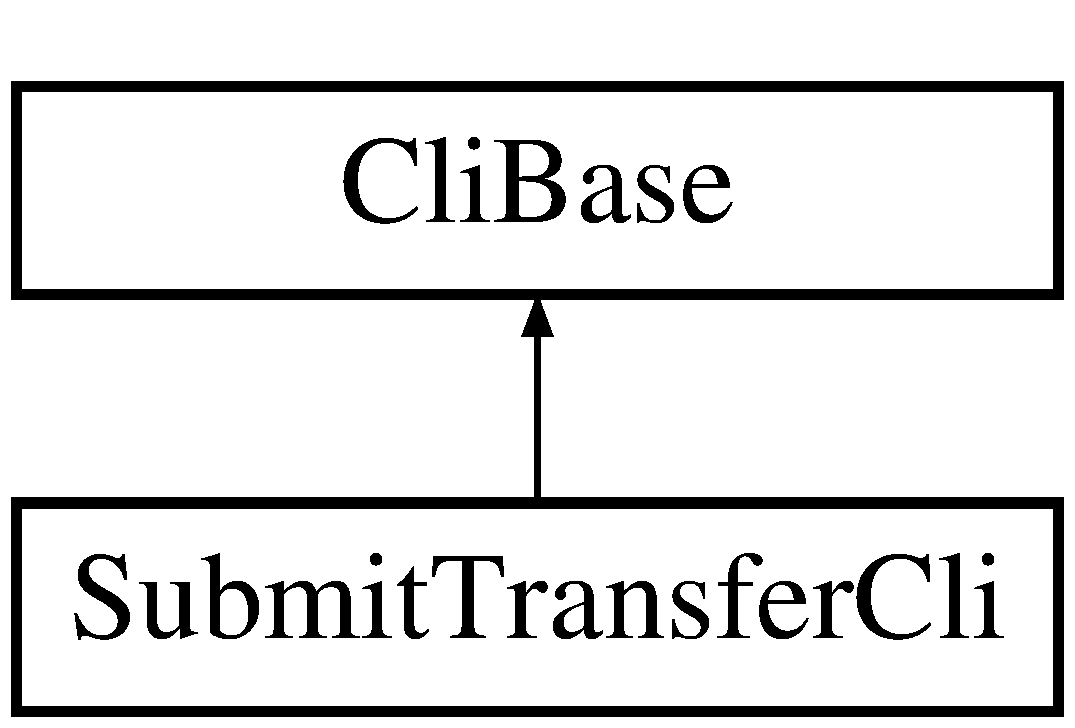
\includegraphics[height=2.000000cm]{classSubmitTransferCli}
\end{center}
\end{figure}
\subsection*{Public Member Functions}
\begin{DoxyCompactItemize}
\item 
{\bf transfer\_\-\_\-TransferParams} $\ast$ {\bfseries getParams} (soap $\ast$soap)\label{classSubmitTransferCli_a5218c8eae866bfeb32ed473d816f3b05}

\item 
bool {\bfseries performChecks} ()\label{classSubmitTransferCli_a33e8547c18b952b96a052eb546f0fc08}

\item 
virtual void {\bfseries initCli} (int ac, char $\ast$av[$\,$])\label{classSubmitTransferCli_ae6dc89c8f7ed9ada6d398195617d9f64}

\item 
string {\bfseries getPassword} ()\label{classSubmitTransferCli_ab3aa66652d42f9ec6953e3bd928f60f6}

\end{DoxyCompactItemize}


\subsection{Detailed Description}


Definition at line 15 of file SubmitTransferCli.h.



The documentation for this class was generated from the following files:\begin{DoxyCompactItemize}
\item 
src/CLI/SubmitTransferCli.h\item 
src/CLI/SubmitTransferCli.cpp\end{DoxyCompactItemize}

\section{transfer\_\-\_\-AuthorizationException Class Reference}
\label{classtransfer____AuthorizationException}\index{transfer\_\-\_\-AuthorizationException@{transfer\_\-\_\-AuthorizationException}}


\char`\"{}http://transfer.data.glite.org\char`\"{}:AuthorizationException is a complexType with complexContent extension of \char`\"{}http://transfer.data.glite.org\char`\"{}:TransferException.  




{\ttfamily \#include $<$fts3-\/transfer-\/submit.h$>$}

Inheritance diagram for transfer\_\-\_\-AuthorizationException:\begin{figure}[H]
\begin{center}
\leavevmode
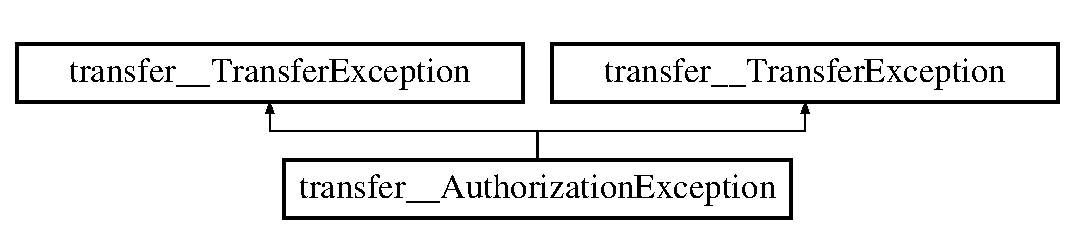
\includegraphics[height=2.000000cm]{classtransfer____AuthorizationException}
\end{center}
\end{figure}
\subsection*{Public Member Functions}
\begin{DoxyCompactItemize}
\item 
virtual int {\bfseries soap\_\-type} () const \label{classtransfer____AuthorizationException_adc826c75f287d7cff21aa9579d72bc89}

\item 
virtual void {\bfseries soap\_\-default} (struct {\bf soap} $\ast$)\label{classtransfer____AuthorizationException_adba3bf62da124e308aea6c7c3c59558e}

\item 
virtual void {\bfseries soap\_\-serialize} (struct {\bf soap} $\ast$) const \label{classtransfer____AuthorizationException_a77409bce93bdcc9bca745b15cf8fc9bb}

\item 
virtual int {\bfseries soap\_\-put} (struct {\bf soap} $\ast$, const char $\ast$, const char $\ast$) const \label{classtransfer____AuthorizationException_ac5666af2a4a9b19689c524a8b5048e8d}

\item 
virtual int {\bfseries soap\_\-out} (struct {\bf soap} $\ast$, const char $\ast$, int, const char $\ast$) const \label{classtransfer____AuthorizationException_aad725d8d5946bba867a986cb867c6faa}

\item 
virtual void $\ast$ {\bfseries soap\_\-get} (struct {\bf soap} $\ast$, const char $\ast$, const char $\ast$)\label{classtransfer____AuthorizationException_a92bd05123a85131551627807473ff8bb}

\item 
virtual void $\ast$ {\bfseries soap\_\-in} (struct {\bf soap} $\ast$, const char $\ast$, const char $\ast$)\label{classtransfer____AuthorizationException_ad3a77ae0706255a3a7ec445ae04d86d6}

\end{DoxyCompactItemize}


\subsection{Detailed Description}
\char`\"{}http://transfer.data.glite.org\char`\"{}:AuthorizationException is a complexType with complexContent extension of \char`\"{}http://transfer.data.glite.org\char`\"{}:TransferException. 

Definition at line 390 of file fts3-\/transfer-\/submit.h.



The documentation for this class was generated from the following files:\begin{DoxyCompactItemize}
\item 
src/CLI/fts3-\/transfer-\/submit.h\item 
src/CLI/ftsStub.h\item 
src/CLI/ftsC.cpp\end{DoxyCompactItemize}

\section{transfer\_\-\_\-CannotCancelException Class Reference}
\label{classtransfer____CannotCancelException}\index{transfer\_\-\_\-CannotCancelException@{transfer\_\-\_\-CannotCancelException}}


\char`\"{}http://transfer.data.glite.org\char`\"{}:CannotCancelException is a complexType with complexContent extension of \char`\"{}http://transfer.data.glite.org\char`\"{}:TransferException.  




{\ttfamily \#include $<$fts3-\/transfer-\/submit.h$>$}

Inheritance diagram for transfer\_\-\_\-CannotCancelException:\begin{figure}[H]
\begin{center}
\leavevmode
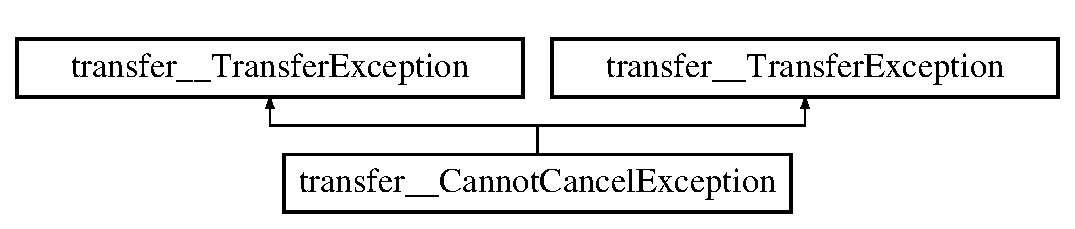
\includegraphics[height=2.000000cm]{classtransfer____CannotCancelException}
\end{center}
\end{figure}
\subsection*{Public Member Functions}
\begin{DoxyCompactItemize}
\item 
virtual int {\bfseries soap\_\-type} () const \label{classtransfer____CannotCancelException_ab953cb376a836476fb23c9bf855401ff}

\item 
virtual void {\bfseries soap\_\-default} (struct {\bf soap} $\ast$)\label{classtransfer____CannotCancelException_a717c02200f3bfb47785935cb8fa8bf2b}

\item 
virtual void {\bfseries soap\_\-serialize} (struct {\bf soap} $\ast$) const \label{classtransfer____CannotCancelException_ac86bfb9ea965616548caaf04d533c5ad}

\item 
virtual int {\bfseries soap\_\-put} (struct {\bf soap} $\ast$, const char $\ast$, const char $\ast$) const \label{classtransfer____CannotCancelException_a69850bc3a5b33935700e2046815a0b4f}

\item 
virtual int {\bfseries soap\_\-out} (struct {\bf soap} $\ast$, const char $\ast$, int, const char $\ast$) const \label{classtransfer____CannotCancelException_aeebb2aa0681ea673fcba0ca672bf1563}

\item 
virtual void $\ast$ {\bfseries soap\_\-get} (struct {\bf soap} $\ast$, const char $\ast$, const char $\ast$)\label{classtransfer____CannotCancelException_a2b777f0e87d99d5ba1b872fbb0c30877}

\item 
virtual void $\ast$ {\bfseries soap\_\-in} (struct {\bf soap} $\ast$, const char $\ast$, const char $\ast$)\label{classtransfer____CannotCancelException_adb888139043e643b36e42b719dc293df}

\end{DoxyCompactItemize}


\subsection{Detailed Description}
\char`\"{}http://transfer.data.glite.org\char`\"{}:CannotCancelException is a complexType with complexContent extension of \char`\"{}http://transfer.data.glite.org\char`\"{}:TransferException. 

Definition at line 500 of file fts3-\/transfer-\/submit.h.



The documentation for this class was generated from the following files:\begin{DoxyCompactItemize}
\item 
src/CLI/fts3-\/transfer-\/submit.h\item 
src/CLI/ftsStub.h\item 
src/CLI/ftsC.cpp\end{DoxyCompactItemize}

\section{transfer\_\-\_\-ExistsException Class Reference}
\label{classtransfer____ExistsException}\index{transfer\_\-\_\-ExistsException@{transfer\_\-\_\-ExistsException}}


\char`\"{}http://transfer.data.glite.org\char`\"{}:ExistsException is a complexType with complexContent extension of \char`\"{}http://transfer.data.glite.org\char`\"{}:TransferException.  




{\ttfamily \#include $<$fts3-\/transfer-\/submit.h$>$}

Inheritance diagram for transfer\_\-\_\-ExistsException:\begin{figure}[H]
\begin{center}
\leavevmode
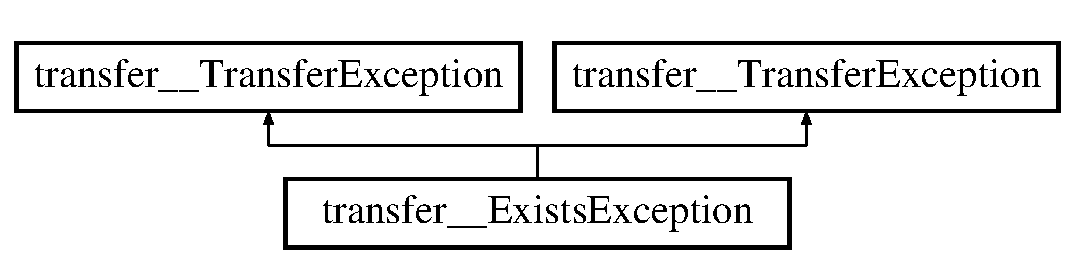
\includegraphics[height=2.000000cm]{classtransfer____ExistsException}
\end{center}
\end{figure}
\subsection*{Public Member Functions}
\begin{DoxyCompactItemize}
\item 
virtual int {\bfseries soap\_\-type} () const \label{classtransfer____ExistsException_aab0cb74d2b9fa9a09b9001d6edbcb5c9}

\item 
virtual void {\bfseries soap\_\-default} (struct {\bf soap} $\ast$)\label{classtransfer____ExistsException_a862e4c622d5d767654ce249beb28b1f5}

\item 
virtual void {\bfseries soap\_\-serialize} (struct {\bf soap} $\ast$) const \label{classtransfer____ExistsException_af2dab9b991dab55caf5a3a9cd889c98d}

\item 
virtual int {\bfseries soap\_\-put} (struct {\bf soap} $\ast$, const char $\ast$, const char $\ast$) const \label{classtransfer____ExistsException_a6fe097bf3b01663bac80fe1528d544d8}

\item 
virtual int {\bfseries soap\_\-out} (struct {\bf soap} $\ast$, const char $\ast$, int, const char $\ast$) const \label{classtransfer____ExistsException_ab6203c01116d7206b28be4101bdbc77f}

\item 
virtual void $\ast$ {\bfseries soap\_\-get} (struct {\bf soap} $\ast$, const char $\ast$, const char $\ast$)\label{classtransfer____ExistsException_af350641b05672db2db3c72be655ffc64}

\item 
virtual void $\ast$ {\bfseries soap\_\-in} (struct {\bf soap} $\ast$, const char $\ast$, const char $\ast$)\label{classtransfer____ExistsException_a334ea62a90cab00abb84c2ce7ce34f1e}

\end{DoxyCompactItemize}


\subsection{Detailed Description}
\char`\"{}http://transfer.data.glite.org\char`\"{}:ExistsException is a complexType with complexContent extension of \char`\"{}http://transfer.data.glite.org\char`\"{}:TransferException. 

Definition at line 509 of file fts3-\/transfer-\/submit.h.



The documentation for this class was generated from the following files:\begin{DoxyCompactItemize}
\item 
src/CLI/fts3-\/transfer-\/submit.h\item 
src/CLI/ftsStub.h\item 
src/CLI/ftsC.cpp\end{DoxyCompactItemize}

\section{transfer\_\-\_\-FileTransferStatus Class Reference}
\label{classtransfer____FileTransferStatus}\index{transfer\_\-\_\-FileTransferStatus@{transfer\_\-\_\-FileTransferStatus}}


\char`\"{}http://transfer.data.glite.org\char`\"{}:FileTransferStatus is a complexType.  




{\ttfamily \#include $<$fts3-\/transfer-\/submit.h$>$}

Inheritance diagram for transfer\_\-\_\-FileTransferStatus:\begin{figure}[H]
\begin{center}
\leavevmode
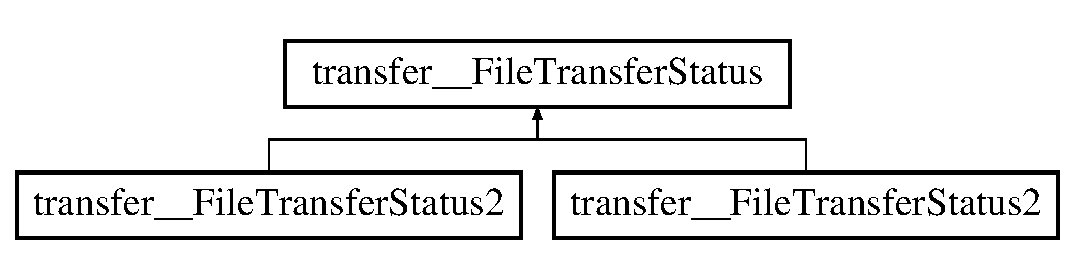
\includegraphics[height=2.000000cm]{classtransfer____FileTransferStatus}
\end{center}
\end{figure}
\subsection*{Public Member Functions}
\begin{DoxyCompactItemize}
\item 
virtual int {\bfseries soap\_\-type} () const \label{classtransfer____FileTransferStatus_a642ad3383ab927add4be60c6f333598a}

\item 
virtual void {\bfseries soap\_\-default} (struct {\bf soap} $\ast$)\label{classtransfer____FileTransferStatus_a888fcc282ac6ee23e00f9a5f8ee03a97}

\item 
virtual void {\bfseries soap\_\-serialize} (struct {\bf soap} $\ast$) const \label{classtransfer____FileTransferStatus_a84c43b07cef43be53d63cd90fe18fa8c}

\item 
virtual int {\bfseries soap\_\-put} (struct {\bf soap} $\ast$, const char $\ast$, const char $\ast$) const \label{classtransfer____FileTransferStatus_adb8ca349c5e0c04e5848729f4d8dafb7}

\item 
virtual int {\bfseries soap\_\-out} (struct {\bf soap} $\ast$, const char $\ast$, int, const char $\ast$) const \label{classtransfer____FileTransferStatus_a6320b08bede2ce96dc59d3de61d95a96}

\item 
virtual void $\ast$ {\bfseries soap\_\-get} (struct {\bf soap} $\ast$, const char $\ast$, const char $\ast$)\label{classtransfer____FileTransferStatus_a8d67affe727870fea60c679ccf0207bb}

\item 
virtual void $\ast$ {\bfseries soap\_\-in} (struct {\bf soap} $\ast$, const char $\ast$, const char $\ast$)\label{classtransfer____FileTransferStatus_aee03aa44cbdbf4606d21109433facaae}

\end{DoxyCompactItemize}
\subsection*{Data Fields}
\begin{DoxyCompactItemize}
\item 
std::string $\ast$ {\bf logicalName}
\begin{DoxyCompactList}\small\item\em Element logicalName of type xs:string. \item\end{DoxyCompactList}\item 
std::string $\ast$ {\bf sourceSURL}
\begin{DoxyCompactList}\small\item\em Element sourceSURL of type xs:string. \item\end{DoxyCompactList}\item 
std::string $\ast$ {\bf destSURL}
\begin{DoxyCompactList}\small\item\em Element destSURL of type xs:string. \item\end{DoxyCompactList}\item 
std::string $\ast$ {\bf transferFileState}
\begin{DoxyCompactList}\small\item\em Element transferFileState of type xs:string. \item\end{DoxyCompactList}\item 
int {\bf numFailures}
\begin{DoxyCompactList}\small\item\em Element numFailures of type xs:int. \item\end{DoxyCompactList}\item 
std::string $\ast$ {\bf reason}
\begin{DoxyCompactList}\small\item\em Element reason of type xs:string. \item\end{DoxyCompactList}\item 
std::string $\ast$ {\bf reason\_\-USCOREclass}
\begin{DoxyCompactList}\small\item\em Element reason\_\-class of type xs:string. \item\end{DoxyCompactList}\item 
LONG64 {\bf duration}
\begin{DoxyCompactList}\small\item\em Element duration of type xs:long. \item\end{DoxyCompactList}\item 
struct {\bf soap} $\ast$ {\bf soap}\label{classtransfer____FileTransferStatus_ac370aec106125a2bdca5ef67bed75868}

\begin{DoxyCompactList}\small\item\em A handle to the soap struct that manages this instance (automatically set) \item\end{DoxyCompactList}\end{DoxyCompactItemize}


\subsection{Detailed Description}
\char`\"{}http://transfer.data.glite.org\char`\"{}:FileTransferStatus is a complexType. 

Definition at line 263 of file fts3-\/transfer-\/submit.h.



\subsection{Field Documentation}
\index{transfer\_\-\_\-FileTransferStatus@{transfer\_\-\_\-FileTransferStatus}!destSURL@{destSURL}}
\index{destSURL@{destSURL}!transfer__FileTransferStatus@{transfer\_\-\_\-FileTransferStatus}}
\subsubsection[{destSURL}]{\setlength{\rightskip}{0pt plus 5cm}std::string $\ast$ {\bf transfer\_\-\_\-FileTransferStatus::destSURL}}\label{classtransfer____FileTransferStatus_a350d3ba3d24685a4decd929d2c0deab7}


Element destSURL of type xs:string. 

Nullable pointer. 

Definition at line 270 of file fts3-\/transfer-\/submit.h.

\index{transfer\_\-\_\-FileTransferStatus@{transfer\_\-\_\-FileTransferStatus}!duration@{duration}}
\index{duration@{duration}!transfer__FileTransferStatus@{transfer\_\-\_\-FileTransferStatus}}
\subsubsection[{duration}]{\setlength{\rightskip}{0pt plus 5cm}LONG64 {\bf transfer\_\-\_\-FileTransferStatus::duration}}\label{classtransfer____FileTransferStatus_a8b0726ff54bc997e0ad3b55c62da196a}


Element duration of type xs:long. 

Required element. 

Definition at line 280 of file fts3-\/transfer-\/submit.h.

\index{transfer\_\-\_\-FileTransferStatus@{transfer\_\-\_\-FileTransferStatus}!logicalName@{logicalName}}
\index{logicalName@{logicalName}!transfer__FileTransferStatus@{transfer\_\-\_\-FileTransferStatus}}
\subsubsection[{logicalName}]{\setlength{\rightskip}{0pt plus 5cm}std::string $\ast$ {\bf transfer\_\-\_\-FileTransferStatus::logicalName}}\label{classtransfer____FileTransferStatus_ae28af9f2eadc5038ab3b4858bcd74a46}


Element logicalName of type xs:string. 

Nullable pointer. 

Definition at line 266 of file fts3-\/transfer-\/submit.h.

\index{transfer\_\-\_\-FileTransferStatus@{transfer\_\-\_\-FileTransferStatus}!numFailures@{numFailures}}
\index{numFailures@{numFailures}!transfer__FileTransferStatus@{transfer\_\-\_\-FileTransferStatus}}
\subsubsection[{numFailures}]{\setlength{\rightskip}{0pt plus 5cm}int {\bf transfer\_\-\_\-FileTransferStatus::numFailures}}\label{classtransfer____FileTransferStatus_a5ff74ed73072e23d7ccb64c6adfbd7be}


Element numFailures of type xs:int. 

Required element. 

Definition at line 274 of file fts3-\/transfer-\/submit.h.

\index{transfer\_\-\_\-FileTransferStatus@{transfer\_\-\_\-FileTransferStatus}!reason@{reason}}
\index{reason@{reason}!transfer__FileTransferStatus@{transfer\_\-\_\-FileTransferStatus}}
\subsubsection[{reason}]{\setlength{\rightskip}{0pt plus 5cm}std::string $\ast$ {\bf transfer\_\-\_\-FileTransferStatus::reason}}\label{classtransfer____FileTransferStatus_a6731977e9f161be9dd2b0d5643d62b3c}


Element reason of type xs:string. 

Nullable pointer. 

Definition at line 276 of file fts3-\/transfer-\/submit.h.

\index{transfer\_\-\_\-FileTransferStatus@{transfer\_\-\_\-FileTransferStatus}!reason\_\-USCOREclass@{reason\_\-USCOREclass}}
\index{reason\_\-USCOREclass@{reason\_\-USCOREclass}!transfer__FileTransferStatus@{transfer\_\-\_\-FileTransferStatus}}
\subsubsection[{reason\_\-USCOREclass}]{\setlength{\rightskip}{0pt plus 5cm}std::string $\ast$ {\bf transfer\_\-\_\-FileTransferStatus::reason\_\-USCOREclass}}\label{classtransfer____FileTransferStatus_a0b9fa91c980937fa104d377a84147dd7}


Element reason\_\-class of type xs:string. 

Nullable pointer. 

Definition at line 278 of file fts3-\/transfer-\/submit.h.

\index{transfer\_\-\_\-FileTransferStatus@{transfer\_\-\_\-FileTransferStatus}!sourceSURL@{sourceSURL}}
\index{sourceSURL@{sourceSURL}!transfer__FileTransferStatus@{transfer\_\-\_\-FileTransferStatus}}
\subsubsection[{sourceSURL}]{\setlength{\rightskip}{0pt plus 5cm}std::string $\ast$ {\bf transfer\_\-\_\-FileTransferStatus::sourceSURL}}\label{classtransfer____FileTransferStatus_a290772d67cc660d332400efa839b2081}


Element sourceSURL of type xs:string. 

Nullable pointer. 

Definition at line 268 of file fts3-\/transfer-\/submit.h.

\index{transfer\_\-\_\-FileTransferStatus@{transfer\_\-\_\-FileTransferStatus}!transferFileState@{transferFileState}}
\index{transferFileState@{transferFileState}!transfer__FileTransferStatus@{transfer\_\-\_\-FileTransferStatus}}
\subsubsection[{transferFileState}]{\setlength{\rightskip}{0pt plus 5cm}std::string $\ast$ {\bf transfer\_\-\_\-FileTransferStatus::transferFileState}}\label{classtransfer____FileTransferStatus_a87df9ec0e5ec3d6881ef5b95088a77e7}


Element transferFileState of type xs:string. 

Nullable pointer. 

Definition at line 272 of file fts3-\/transfer-\/submit.h.



The documentation for this class was generated from the following files:\begin{DoxyCompactItemize}
\item 
src/CLI/fts3-\/transfer-\/submit.h\item 
src/CLI/ftsStub.h\item 
src/CLI/ftsC.cpp\end{DoxyCompactItemize}

\section{transfer\_\-\_\-FileTransferStatus2 Class Reference}
\label{classtransfer____FileTransferStatus2}\index{transfer\_\-\_\-FileTransferStatus2@{transfer\_\-\_\-FileTransferStatus2}}


\char`\"{}http://transfer.data.glite.org\char`\"{}:FileTransferStatus2 is a complexType with complexContent extension of \char`\"{}http://transfer.data.glite.org\char`\"{}:FileTransferStatus.  




{\ttfamily \#include $<$fts3-\/transfer-\/submit.h$>$}

Inheritance diagram for transfer\_\-\_\-FileTransferStatus2:\begin{figure}[H]
\begin{center}
\leavevmode
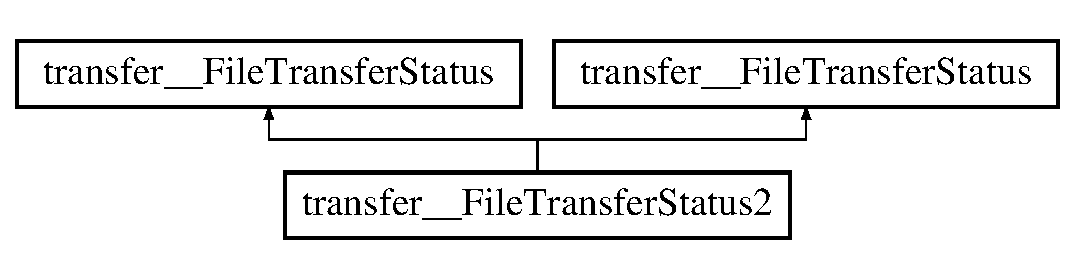
\includegraphics[height=2.000000cm]{classtransfer____FileTransferStatus2}
\end{center}
\end{figure}
\subsection*{Public Member Functions}
\begin{DoxyCompactItemize}
\item 
virtual int {\bfseries soap\_\-type} () const \label{classtransfer____FileTransferStatus2_ade3559547f4e61deb23e63e1b3266cc9}

\item 
virtual void {\bfseries soap\_\-default} (struct {\bf soap} $\ast$)\label{classtransfer____FileTransferStatus2_a90c52f3be885acd7affb97629787774e}

\item 
virtual void {\bfseries soap\_\-serialize} (struct {\bf soap} $\ast$) const \label{classtransfer____FileTransferStatus2_a9bf9d6304a7d975516e2db07f4bfd883}

\item 
virtual int {\bfseries soap\_\-put} (struct {\bf soap} $\ast$, const char $\ast$, const char $\ast$) const \label{classtransfer____FileTransferStatus2_a1812dcece75c2acba545ea6b93134108}

\item 
virtual int {\bfseries soap\_\-out} (struct {\bf soap} $\ast$, const char $\ast$, int, const char $\ast$) const \label{classtransfer____FileTransferStatus2_a43e1179a6657b04e56b0b27c9e389e3e}

\item 
virtual void $\ast$ {\bfseries soap\_\-get} (struct {\bf soap} $\ast$, const char $\ast$, const char $\ast$)\label{classtransfer____FileTransferStatus2_ab298f85f3d52ff1b06785606b1381b7c}

\item 
virtual void $\ast$ {\bfseries soap\_\-in} (struct {\bf soap} $\ast$, const char $\ast$, const char $\ast$)\label{classtransfer____FileTransferStatus2_ae618347ccaf53da1a223cb52b42138f7}

\end{DoxyCompactItemize}
\subsection*{Data Fields}
\begin{DoxyCompactItemize}
\item 
std::string $\ast$ {\bf error\_\-USCOREscope}
\begin{DoxyCompactList}\small\item\em Element error\_\-scope of type xs:string. \item\end{DoxyCompactList}\item 
std::string $\ast$ {\bf error\_\-USCOREphase}
\begin{DoxyCompactList}\small\item\em Element error\_\-phase of type xs:string. \item\end{DoxyCompactList}\end{DoxyCompactItemize}


\subsection{Detailed Description}
\char`\"{}http://transfer.data.glite.org\char`\"{}:FileTransferStatus2 is a complexType with complexContent extension of \char`\"{}http://transfer.data.glite.org\char`\"{}:FileTransferStatus. 

Definition at line 426 of file fts3-\/transfer-\/submit.h.



\subsection{Field Documentation}
\index{transfer\_\-\_\-FileTransferStatus2@{transfer\_\-\_\-FileTransferStatus2}!error\_\-USCOREphase@{error\_\-USCOREphase}}
\index{error\_\-USCOREphase@{error\_\-USCOREphase}!transfer__FileTransferStatus2@{transfer\_\-\_\-FileTransferStatus2}}
\subsubsection[{error\_\-USCOREphase}]{\setlength{\rightskip}{0pt plus 5cm}std::string $\ast$ {\bf transfer\_\-\_\-FileTransferStatus2::error\_\-USCOREphase}}\label{classtransfer____FileTransferStatus2_ac854f3d552f37da65996694a526dd1fe}


Element error\_\-phase of type xs:string. 

Nullable pointer. 

Definition at line 449 of file fts3-\/transfer-\/submit.h.

\index{transfer\_\-\_\-FileTransferStatus2@{transfer\_\-\_\-FileTransferStatus2}!error\_\-USCOREscope@{error\_\-USCOREscope}}
\index{error\_\-USCOREscope@{error\_\-USCOREscope}!transfer__FileTransferStatus2@{transfer\_\-\_\-FileTransferStatus2}}
\subsubsection[{error\_\-USCOREscope}]{\setlength{\rightskip}{0pt plus 5cm}std::string $\ast$ {\bf transfer\_\-\_\-FileTransferStatus2::error\_\-USCOREscope}}\label{classtransfer____FileTransferStatus2_ad90e6aa496483063209a31faa8a80b97}


Element error\_\-scope of type xs:string. 

Nullable pointer. 

Definition at line 447 of file fts3-\/transfer-\/submit.h.



The documentation for this class was generated from the following files:\begin{DoxyCompactItemize}
\item 
src/CLI/fts3-\/transfer-\/submit.h\item 
src/CLI/ftsStub.h\item 
src/CLI/ftsC.cpp\end{DoxyCompactItemize}

\section{transfer\_\-\_\-InternalException Class Reference}
\label{classtransfer____InternalException}\index{transfer\_\-\_\-InternalException@{transfer\_\-\_\-InternalException}}


\char`\"{}http://transfer.data.glite.org\char`\"{}:InternalException is a complexType with complexContent extension of \char`\"{}http://transfer.data.glite.org\char`\"{}:TransferException.  




{\ttfamily \#include $<$fts3-\/transfer-\/submit.h$>$}

Inheritance diagram for transfer\_\-\_\-InternalException:\begin{figure}[H]
\begin{center}
\leavevmode
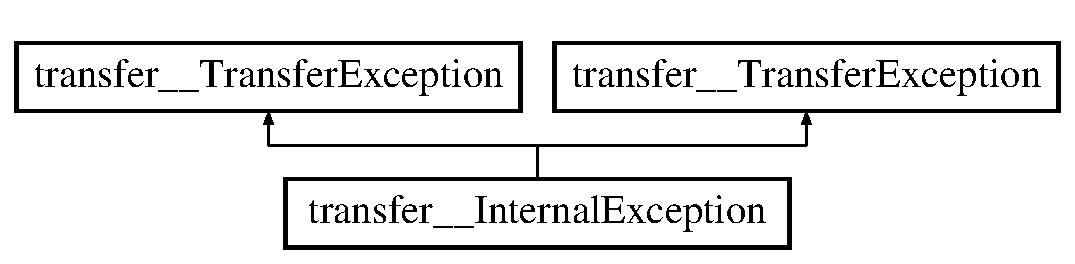
\includegraphics[height=2.000000cm]{classtransfer____InternalException}
\end{center}
\end{figure}
\subsection*{Public Member Functions}
\begin{DoxyCompactItemize}
\item 
virtual int {\bfseries soap\_\-type} () const \label{classtransfer____InternalException_ad36b4d393190a19a4e40975412f10f49}

\item 
virtual void {\bfseries soap\_\-default} (struct {\bf soap} $\ast$)\label{classtransfer____InternalException_a25c52a9a180076f8990925a704250057}

\item 
virtual void {\bfseries soap\_\-serialize} (struct {\bf soap} $\ast$) const \label{classtransfer____InternalException_a16c4ef97ab32a82a81134209f15cbeef}

\item 
virtual int {\bfseries soap\_\-put} (struct {\bf soap} $\ast$, const char $\ast$, const char $\ast$) const \label{classtransfer____InternalException_a7fd18b08645fdf057124a46636dabb7e}

\item 
virtual int {\bfseries soap\_\-out} (struct {\bf soap} $\ast$, const char $\ast$, int, const char $\ast$) const \label{classtransfer____InternalException_a72c8515e9b66d1811406ea1a7527cb1a}

\item 
virtual void $\ast$ {\bfseries soap\_\-get} (struct {\bf soap} $\ast$, const char $\ast$, const char $\ast$)\label{classtransfer____InternalException_a4c02c9387e0cb377385ae4cf29794082}

\item 
virtual void $\ast$ {\bfseries soap\_\-in} (struct {\bf soap} $\ast$, const char $\ast$, const char $\ast$)\label{classtransfer____InternalException_a1321c2af78292cb5310c3b659e48a758}

\end{DoxyCompactItemize}


\subsection{Detailed Description}
\char`\"{}http://transfer.data.glite.org\char`\"{}:InternalException is a complexType with complexContent extension of \char`\"{}http://transfer.data.glite.org\char`\"{}:TransferException. 

Definition at line 408 of file fts3-\/transfer-\/submit.h.



The documentation for this class was generated from the following files:\begin{DoxyCompactItemize}
\item 
src/CLI/fts3-\/transfer-\/submit.h\item 
src/CLI/ftsStub.h\item 
src/CLI/ftsC.cpp\end{DoxyCompactItemize}

\section{transfer\_\-\_\-InvalidArgumentException Class Reference}
\label{classtransfer____InvalidArgumentException}\index{transfer\_\-\_\-InvalidArgumentException@{transfer\_\-\_\-InvalidArgumentException}}


\char`\"{}http://transfer.data.glite.org\char`\"{}:InvalidArgumentException is a complexType with complexContent extension of \char`\"{}http://transfer.data.glite.org\char`\"{}:TransferException.  




{\ttfamily \#include $<$fts3-\/transfer-\/submit.h$>$}

Inheritance diagram for transfer\_\-\_\-InvalidArgumentException:\begin{figure}[H]
\begin{center}
\leavevmode
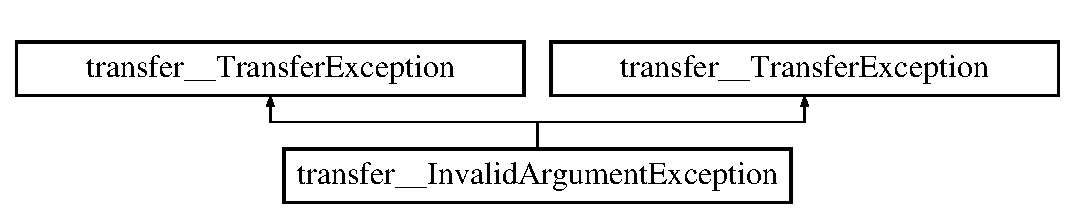
\includegraphics[height=2.000000cm]{classtransfer____InvalidArgumentException}
\end{center}
\end{figure}
\subsection*{Public Member Functions}
\begin{DoxyCompactItemize}
\item 
virtual int {\bfseries soap\_\-type} () const \label{classtransfer____InvalidArgumentException_af13c682aa8ac06c0d7a7159d69ce4466}

\item 
virtual void {\bfseries soap\_\-default} (struct {\bf soap} $\ast$)\label{classtransfer____InvalidArgumentException_a471166c8b37d36c458bd0a4b8f770953}

\item 
virtual void {\bfseries soap\_\-serialize} (struct {\bf soap} $\ast$) const \label{classtransfer____InvalidArgumentException_a0bfedaac6062e26620f2630a8c004845}

\item 
virtual int {\bfseries soap\_\-put} (struct {\bf soap} $\ast$, const char $\ast$, const char $\ast$) const \label{classtransfer____InvalidArgumentException_a30752da402add21fc7d592c8e276a82e}

\item 
virtual int {\bfseries soap\_\-out} (struct {\bf soap} $\ast$, const char $\ast$, int, const char $\ast$) const \label{classtransfer____InvalidArgumentException_a62a1cae6327c51207ee37575ca2b579d}

\item 
virtual void $\ast$ {\bfseries soap\_\-get} (struct {\bf soap} $\ast$, const char $\ast$, const char $\ast$)\label{classtransfer____InvalidArgumentException_a621dc17c143b729f6446a1e88ac9b0b1}

\item 
virtual void $\ast$ {\bfseries soap\_\-in} (struct {\bf soap} $\ast$, const char $\ast$, const char $\ast$)\label{classtransfer____InvalidArgumentException_aae6ee95918d3784d35cda75b5c70d954}

\end{DoxyCompactItemize}


\subsection{Detailed Description}
\char`\"{}http://transfer.data.glite.org\char`\"{}:InvalidArgumentException is a complexType with complexContent extension of \char`\"{}http://transfer.data.glite.org\char`\"{}:TransferException. 

Definition at line 381 of file fts3-\/transfer-\/submit.h.



The documentation for this class was generated from the following files:\begin{DoxyCompactItemize}
\item 
src/CLI/fts3-\/transfer-\/submit.h\item 
src/CLI/ftsStub.h\item 
src/CLI/ftsC.cpp\end{DoxyCompactItemize}

\section{transfer\_\-\_\-JobStatus Class Reference}
\label{classtransfer____JobStatus}\index{transfer\_\-\_\-JobStatus@{transfer\_\-\_\-JobStatus}}


\char`\"{}http://transfer.data.glite.org\char`\"{}:JobStatus is a complexType.  




{\ttfamily \#include $<$fts3-\/transfer-\/submit.h$>$}

\subsection*{Public Member Functions}
\begin{DoxyCompactItemize}
\item 
virtual int {\bfseries soap\_\-type} () const \label{classtransfer____JobStatus_adf3c576598572fc4ef23425136034da6}

\item 
virtual void {\bfseries soap\_\-default} (struct {\bf soap} $\ast$)\label{classtransfer____JobStatus_ab2066b2d6e93b4ddbdb494dc00957411}

\item 
virtual void {\bfseries soap\_\-serialize} (struct {\bf soap} $\ast$) const \label{classtransfer____JobStatus_a59955cd1d7800231b9e1bb42a4c8fe74}

\item 
virtual int {\bfseries soap\_\-put} (struct {\bf soap} $\ast$, const char $\ast$, const char $\ast$) const \label{classtransfer____JobStatus_aea9fe3403040242176130c4b5cbb78bf}

\item 
virtual int {\bfseries soap\_\-out} (struct {\bf soap} $\ast$, const char $\ast$, int, const char $\ast$) const \label{classtransfer____JobStatus_a31bacb77f8ced8a26ef3c3ad9c2cf7c1}

\item 
virtual void $\ast$ {\bfseries soap\_\-get} (struct {\bf soap} $\ast$, const char $\ast$, const char $\ast$)\label{classtransfer____JobStatus_a173df825f18c08ec4d828834aac7f890}

\item 
virtual void $\ast$ {\bfseries soap\_\-in} (struct {\bf soap} $\ast$, const char $\ast$, const char $\ast$)\label{classtransfer____JobStatus_a379591ad7d9c0468b358d3ad8f0e31c1}

\end{DoxyCompactItemize}
\subsection*{Data Fields}
\begin{DoxyCompactItemize}
\item 
std::string $\ast$ {\bf jobID}
\begin{DoxyCompactList}\small\item\em Element jobID of type xs:string. \item\end{DoxyCompactList}\item 
std::string $\ast$ {\bf jobStatus}
\begin{DoxyCompactList}\small\item\em Element jobStatus of type xs:string. \item\end{DoxyCompactList}\item 
std::string $\ast$ {\bf clientDN}
\begin{DoxyCompactList}\small\item\em Element clientDN of type xs:string. \item\end{DoxyCompactList}\item 
std::string $\ast$ {\bf reason}
\begin{DoxyCompactList}\small\item\em Element reason of type xs:string. \item\end{DoxyCompactList}\item 
std::string $\ast$ {\bf voName}
\begin{DoxyCompactList}\small\item\em Element voName of type xs:string. \item\end{DoxyCompactList}\item 
LONG64 {\bf submitTime}
\begin{DoxyCompactList}\small\item\em Element submitTime of type xs:long. \item\end{DoxyCompactList}\item 
int {\bf numFiles}
\begin{DoxyCompactList}\small\item\em Element numFiles of type xs:int. \item\end{DoxyCompactList}\item 
int {\bf priority}
\begin{DoxyCompactList}\small\item\em Element priority of type xs:int. \item\end{DoxyCompactList}\item 
struct {\bf soap} $\ast$ {\bf soap}\label{classtransfer____JobStatus_ad58a9cf654b293b8f5115aef6da414f5}

\begin{DoxyCompactList}\small\item\em A handle to the soap struct that manages this instance (automatically set) \item\end{DoxyCompactList}\end{DoxyCompactItemize}


\subsection{Detailed Description}
\char`\"{}http://transfer.data.glite.org\char`\"{}:JobStatus is a complexType. 

Definition at line 240 of file fts3-\/transfer-\/submit.h.



\subsection{Field Documentation}
\index{transfer\_\-\_\-JobStatus@{transfer\_\-\_\-JobStatus}!clientDN@{clientDN}}
\index{clientDN@{clientDN}!transfer__JobStatus@{transfer\_\-\_\-JobStatus}}
\subsubsection[{clientDN}]{\setlength{\rightskip}{0pt plus 5cm}std::string $\ast$ {\bf transfer\_\-\_\-JobStatus::clientDN}}\label{classtransfer____JobStatus_a61202a8e6fd62cd46631b7001981931e}


Element clientDN of type xs:string. 

Nullable pointer. 

Definition at line 247 of file fts3-\/transfer-\/submit.h.

\index{transfer\_\-\_\-JobStatus@{transfer\_\-\_\-JobStatus}!jobID@{jobID}}
\index{jobID@{jobID}!transfer__JobStatus@{transfer\_\-\_\-JobStatus}}
\subsubsection[{jobID}]{\setlength{\rightskip}{0pt plus 5cm}std::string $\ast$ {\bf transfer\_\-\_\-JobStatus::jobID}}\label{classtransfer____JobStatus_af0df3912849c67971cd3148872b8016a}


Element jobID of type xs:string. 

Nullable pointer. 

Definition at line 243 of file fts3-\/transfer-\/submit.h.

\index{transfer\_\-\_\-JobStatus@{transfer\_\-\_\-JobStatus}!jobStatus@{jobStatus}}
\index{jobStatus@{jobStatus}!transfer__JobStatus@{transfer\_\-\_\-JobStatus}}
\subsubsection[{jobStatus}]{\setlength{\rightskip}{0pt plus 5cm}std::string $\ast$ {\bf transfer\_\-\_\-JobStatus::jobStatus}}\label{classtransfer____JobStatus_a7ed5dedbffd7ae5c141b5de6a9220b07}


Element jobStatus of type xs:string. 

Nullable pointer. 

Definition at line 245 of file fts3-\/transfer-\/submit.h.

\index{transfer\_\-\_\-JobStatus@{transfer\_\-\_\-JobStatus}!numFiles@{numFiles}}
\index{numFiles@{numFiles}!transfer__JobStatus@{transfer\_\-\_\-JobStatus}}
\subsubsection[{numFiles}]{\setlength{\rightskip}{0pt plus 5cm}int {\bf transfer\_\-\_\-JobStatus::numFiles}}\label{classtransfer____JobStatus_a969570f12524471b1d9a7dbc30daf7e6}


Element numFiles of type xs:int. 

Required element. 

Definition at line 255 of file fts3-\/transfer-\/submit.h.

\index{transfer\_\-\_\-JobStatus@{transfer\_\-\_\-JobStatus}!priority@{priority}}
\index{priority@{priority}!transfer__JobStatus@{transfer\_\-\_\-JobStatus}}
\subsubsection[{priority}]{\setlength{\rightskip}{0pt plus 5cm}int {\bf transfer\_\-\_\-JobStatus::priority}}\label{classtransfer____JobStatus_a458195eec1320d9c94b3f2a36183b72f}


Element priority of type xs:int. 

Required element. 

Definition at line 257 of file fts3-\/transfer-\/submit.h.

\index{transfer\_\-\_\-JobStatus@{transfer\_\-\_\-JobStatus}!reason@{reason}}
\index{reason@{reason}!transfer__JobStatus@{transfer\_\-\_\-JobStatus}}
\subsubsection[{reason}]{\setlength{\rightskip}{0pt plus 5cm}std::string $\ast$ {\bf transfer\_\-\_\-JobStatus::reason}}\label{classtransfer____JobStatus_aa9c0c83f99ebff125f9852cbb24b40aa}


Element reason of type xs:string. 

Nullable pointer. 

Definition at line 249 of file fts3-\/transfer-\/submit.h.

\index{transfer\_\-\_\-JobStatus@{transfer\_\-\_\-JobStatus}!submitTime@{submitTime}}
\index{submitTime@{submitTime}!transfer__JobStatus@{transfer\_\-\_\-JobStatus}}
\subsubsection[{submitTime}]{\setlength{\rightskip}{0pt plus 5cm}LONG64 {\bf transfer\_\-\_\-JobStatus::submitTime}}\label{classtransfer____JobStatus_a335aedfcdd9f3cc3fbf7eca50f9a246e}


Element submitTime of type xs:long. 

Required element. 

Definition at line 253 of file fts3-\/transfer-\/submit.h.

\index{transfer\_\-\_\-JobStatus@{transfer\_\-\_\-JobStatus}!voName@{voName}}
\index{voName@{voName}!transfer__JobStatus@{transfer\_\-\_\-JobStatus}}
\subsubsection[{voName}]{\setlength{\rightskip}{0pt plus 5cm}std::string $\ast$ {\bf transfer\_\-\_\-JobStatus::voName}}\label{classtransfer____JobStatus_ada3a67df82deaa29e7cf200e9d9615fe}


Element voName of type xs:string. 

Nullable pointer. 

Definition at line 251 of file fts3-\/transfer-\/submit.h.



The documentation for this class was generated from the following files:\begin{DoxyCompactItemize}
\item 
src/CLI/fts3-\/transfer-\/submit.h\item 
src/CLI/ftsStub.h\item 
src/CLI/ftsC.cpp\end{DoxyCompactItemize}

\section{transfer\_\-\_\-NotExistsException Class Reference}
\label{classtransfer____NotExistsException}\index{transfer\_\-\_\-NotExistsException@{transfer\_\-\_\-NotExistsException}}


\char`\"{}http://transfer.data.glite.org\char`\"{}:NotExistsException is a complexType with complexContent extension of \char`\"{}http://transfer.data.glite.org\char`\"{}:TransferException.  




{\ttfamily \#include $<$fts3-\/transfer-\/submit.h$>$}

Inheritance diagram for transfer\_\-\_\-NotExistsException:\begin{figure}[H]
\begin{center}
\leavevmode
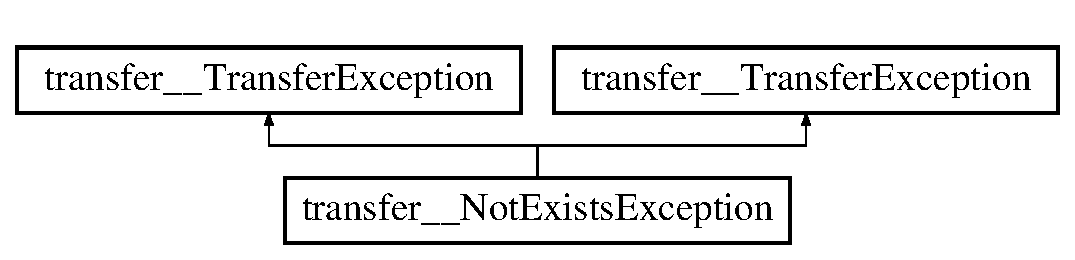
\includegraphics[height=2.000000cm]{classtransfer____NotExistsException}
\end{center}
\end{figure}
\subsection*{Public Member Functions}
\begin{DoxyCompactItemize}
\item 
virtual int {\bfseries soap\_\-type} () const \label{classtransfer____NotExistsException_a81787f77cb069acf938460e5c6c9f7cc}

\item 
virtual void {\bfseries soap\_\-default} (struct {\bf soap} $\ast$)\label{classtransfer____NotExistsException_ae8aec49cc33ebc4bc7084c08ab3cbd6f}

\item 
virtual void {\bfseries soap\_\-serialize} (struct {\bf soap} $\ast$) const \label{classtransfer____NotExistsException_a91e1dc82a7f3f0dc759a709e33b50a19}

\item 
virtual int {\bfseries soap\_\-put} (struct {\bf soap} $\ast$, const char $\ast$, const char $\ast$) const \label{classtransfer____NotExistsException_a52bee29e71eeb837d717717a4da0e96c}

\item 
virtual int {\bfseries soap\_\-out} (struct {\bf soap} $\ast$, const char $\ast$, int, const char $\ast$) const \label{classtransfer____NotExistsException_ada44a95281a7f9759ed32a83bcb953aa}

\item 
virtual void $\ast$ {\bfseries soap\_\-get} (struct {\bf soap} $\ast$, const char $\ast$, const char $\ast$)\label{classtransfer____NotExistsException_a76ab93e4b37c61e2748ce66a5ee57965}

\item 
virtual void $\ast$ {\bfseries soap\_\-in} (struct {\bf soap} $\ast$, const char $\ast$, const char $\ast$)\label{classtransfer____NotExistsException_ada347ffb0653a04752a3de024d266af7}

\end{DoxyCompactItemize}


\subsection{Detailed Description}
\char`\"{}http://transfer.data.glite.org\char`\"{}:NotExistsException is a complexType with complexContent extension of \char`\"{}http://transfer.data.glite.org\char`\"{}:TransferException. 

Definition at line 417 of file fts3-\/transfer-\/submit.h.



The documentation for this class was generated from the following files:\begin{DoxyCompactItemize}
\item 
src/CLI/fts3-\/transfer-\/submit.h\item 
src/CLI/ftsStub.h\item 
src/CLI/ftsC.cpp\end{DoxyCompactItemize}

\section{transfer\_\-\_\-PlacementJob Class Reference}
\label{classtransfer____PlacementJob}\index{transfer\_\-\_\-PlacementJob@{transfer\_\-\_\-PlacementJob}}


\char`\"{}http://transfer.data.glite.org\char`\"{}:PlacementJob is a complexType.  




{\ttfamily \#include $<$fts3-\/transfer-\/submit.h$>$}

\subsection*{Public Member Functions}
\begin{DoxyCompactItemize}
\item 
virtual int {\bfseries soap\_\-type} () const \label{classtransfer____PlacementJob_a0be56c445df6d33a69ed8781ec40d4fa}

\item 
virtual void {\bfseries soap\_\-default} (struct {\bf soap} $\ast$)\label{classtransfer____PlacementJob_a448e5b078c6d6fe135dd7da6949b64b5}

\item 
virtual void {\bfseries soap\_\-serialize} (struct {\bf soap} $\ast$) const \label{classtransfer____PlacementJob_aa11688cb486a61b02c7639268eeba9ae}

\item 
virtual int {\bfseries soap\_\-put} (struct {\bf soap} $\ast$, const char $\ast$, const char $\ast$) const \label{classtransfer____PlacementJob_a39ef8874307babb95c085758e667cfef}

\item 
virtual int {\bfseries soap\_\-out} (struct {\bf soap} $\ast$, const char $\ast$, int, const char $\ast$) const \label{classtransfer____PlacementJob_a55cf5be328877c60a55a9242a51577de}

\item 
virtual void $\ast$ {\bfseries soap\_\-get} (struct {\bf soap} $\ast$, const char $\ast$, const char $\ast$)\label{classtransfer____PlacementJob_a162fa1b623c41a226ecb230f97aed102}

\item 
virtual void $\ast$ {\bfseries soap\_\-in} (struct {\bf soap} $\ast$, const char $\ast$, const char $\ast$)\label{classtransfer____PlacementJob_a948213e07ff28d0457a91250fa572891}

\end{DoxyCompactItemize}
\subsection*{Data Fields}
\begin{DoxyCompactItemize}
\item 
std::vector$<$ std::string $>$ {\bf logicalFiles}
\begin{DoxyCompactList}\small\item\em Vector of std::string with length 1..unbounded. \item\end{DoxyCompactList}\item 
std::string $\ast$ {\bf sourceSE}
\begin{DoxyCompactList}\small\item\em Element sourceSE of type xs:string. \item\end{DoxyCompactList}\item 
std::string $\ast$ {\bf destSE}
\begin{DoxyCompactList}\small\item\em Element destSE of type xs:string. \item\end{DoxyCompactList}\item 
{\bf transfer\_\-\_\-TransferParams} $\ast$ {\bf jobParams}
\begin{DoxyCompactList}\small\item\em Element jobParams of type \char`\"{}http://transfer.data.glite.org\char`\"{}:TransferParams. \item\end{DoxyCompactList}\item 
std::string $\ast$ {\bf credential}
\begin{DoxyCompactList}\small\item\em Element credential of type xs:string. \item\end{DoxyCompactList}\item 
struct {\bf soap} $\ast$ {\bf soap}\label{classtransfer____PlacementJob_a443d5a1ce3cca0448d6ce22479df4425}

\begin{DoxyCompactList}\small\item\em A handle to the soap struct that manages this instance (automatically set) \item\end{DoxyCompactList}\end{DoxyCompactItemize}


\subsection{Detailed Description}
\char`\"{}http://transfer.data.glite.org\char`\"{}:PlacementJob is a complexType. 

Definition at line 164 of file fts3-\/transfer-\/submit.h.



\subsection{Field Documentation}
\index{transfer\_\-\_\-PlacementJob@{transfer\_\-\_\-PlacementJob}!credential@{credential}}
\index{credential@{credential}!transfer__PlacementJob@{transfer\_\-\_\-PlacementJob}}
\subsubsection[{credential}]{\setlength{\rightskip}{0pt plus 5cm}std::string $\ast$ {\bf transfer\_\-\_\-PlacementJob::credential}}\label{classtransfer____PlacementJob_af222e324ccaea32471d6e69e90bb8858}


Element credential of type xs:string. 

Nullable pointer. 

Definition at line 175 of file fts3-\/transfer-\/submit.h.

\index{transfer\_\-\_\-PlacementJob@{transfer\_\-\_\-PlacementJob}!destSE@{destSE}}
\index{destSE@{destSE}!transfer__PlacementJob@{transfer\_\-\_\-PlacementJob}}
\subsubsection[{destSE}]{\setlength{\rightskip}{0pt plus 5cm}std::string $\ast$ {\bf transfer\_\-\_\-PlacementJob::destSE}}\label{classtransfer____PlacementJob_aacb6f1571bc8045734ad8aa27c138c8a}


Element destSE of type xs:string. 

Nullable pointer. 

Definition at line 171 of file fts3-\/transfer-\/submit.h.

\index{transfer\_\-\_\-PlacementJob@{transfer\_\-\_\-PlacementJob}!jobParams@{jobParams}}
\index{jobParams@{jobParams}!transfer__PlacementJob@{transfer\_\-\_\-PlacementJob}}
\subsubsection[{jobParams}]{\setlength{\rightskip}{0pt plus 5cm}{\bf transfer\_\-\_\-TransferParams} $\ast$ {\bf transfer\_\-\_\-PlacementJob::jobParams}}\label{classtransfer____PlacementJob_a83805591f9851821d2d4da834e0b1685}


Element jobParams of type \char`\"{}http://transfer.data.glite.org\char`\"{}:TransferParams. 

Nullable pointer. 

Definition at line 173 of file fts3-\/transfer-\/submit.h.

\index{transfer\_\-\_\-PlacementJob@{transfer\_\-\_\-PlacementJob}!logicalFiles@{logicalFiles}}
\index{logicalFiles@{logicalFiles}!transfer__PlacementJob@{transfer\_\-\_\-PlacementJob}}
\subsubsection[{logicalFiles}]{\setlength{\rightskip}{0pt plus 5cm}std::vector$<$ std::string $>$ {\bf transfer\_\-\_\-PlacementJob::logicalFiles}}\label{classtransfer____PlacementJob_a180ff8c7361bddcbed146216faa8fbeb}


Vector of std::string with length 1..unbounded. 

Nullable pointer. 

Definition at line 167 of file fts3-\/transfer-\/submit.h.

\index{transfer\_\-\_\-PlacementJob@{transfer\_\-\_\-PlacementJob}!sourceSE@{sourceSE}}
\index{sourceSE@{sourceSE}!transfer__PlacementJob@{transfer\_\-\_\-PlacementJob}}
\subsubsection[{sourceSE}]{\setlength{\rightskip}{0pt plus 5cm}std::string $\ast$ {\bf transfer\_\-\_\-PlacementJob::sourceSE}}\label{classtransfer____PlacementJob_adc36949266a8e6b451fc7d9c244f7a61}


Element sourceSE of type xs:string. 

Nullable pointer. 

Definition at line 169 of file fts3-\/transfer-\/submit.h.



The documentation for this class was generated from the following files:\begin{DoxyCompactItemize}
\item 
src/CLI/fts3-\/transfer-\/submit.h\item 
src/CLI/ftsStub.h\item 
src/CLI/ftsC.cpp\end{DoxyCompactItemize}

\section{transfer\_\-\_\-Roles Class Reference}
\label{classtransfer____Roles}\index{transfer\_\-\_\-Roles@{transfer\_\-\_\-Roles}}


\char`\"{}http://transfer.data.glite.org\char`\"{}:Roles is a complexType.  




{\ttfamily \#include $<$fts3-\/transfer-\/submit.h$>$}

\subsection*{Public Member Functions}
\begin{DoxyCompactItemize}
\item 
virtual int {\bfseries soap\_\-type} () const \label{classtransfer____Roles_a3f104a1a66ac503475d31a0a1643d568}

\item 
virtual void {\bfseries soap\_\-default} (struct {\bf soap} $\ast$)\label{classtransfer____Roles_aaad479027cb447922d987270c3356f78}

\item 
virtual void {\bfseries soap\_\-serialize} (struct {\bf soap} $\ast$) const \label{classtransfer____Roles_a3ade19c069d36a9ace4f2cb37cb71efe}

\item 
virtual int {\bfseries soap\_\-put} (struct {\bf soap} $\ast$, const char $\ast$, const char $\ast$) const \label{classtransfer____Roles_a58d2312091b5fec3f28bf83bcaac44ba}

\item 
virtual int {\bfseries soap\_\-out} (struct {\bf soap} $\ast$, const char $\ast$, int, const char $\ast$) const \label{classtransfer____Roles_a1ca1bcdb68b513d50d22b5298b30d54a}

\item 
virtual void $\ast$ {\bfseries soap\_\-get} (struct {\bf soap} $\ast$, const char $\ast$, const char $\ast$)\label{classtransfer____Roles_a270e9e9a2ada3f3cf2caa56a0df29bac}

\item 
virtual void $\ast$ {\bfseries soap\_\-in} (struct {\bf soap} $\ast$, const char $\ast$, const char $\ast$)\label{classtransfer____Roles_a1d4f0f1909403301e0479fffa17f2b6e}

\end{DoxyCompactItemize}
\subsection*{Data Fields}
\begin{DoxyCompactItemize}
\item 
std::string $\ast$ {\bf clientDN}
\begin{DoxyCompactList}\small\item\em Element clientDN of type xs:string. \item\end{DoxyCompactList}\item 
std::string $\ast$ {\bf serviceAdmin}
\begin{DoxyCompactList}\small\item\em Element serviceAdmin of type xs:string. \item\end{DoxyCompactList}\item 
std::string $\ast$ {\bf submitter}
\begin{DoxyCompactList}\small\item\em Element submitter of type xs:string. \item\end{DoxyCompactList}\item 
std::vector$<$ {\bf transfer\_\-\_\-StringPair} $\ast$ $>$ {\bf VOManager}
\begin{DoxyCompactList}\small\item\em Vector of transfer\_\-\_\-StringPair$\ast$ with length 1..unbounded. \item\end{DoxyCompactList}\item 
struct {\bf soap} $\ast$ {\bf soap}\label{classtransfer____Roles_ac9a8fb773fc766a946850cf68711d025}

\begin{DoxyCompactList}\small\item\em A handle to the soap struct that manages this instance (automatically set) \item\end{DoxyCompactList}\end{DoxyCompactItemize}


\subsection{Detailed Description}
\char`\"{}http://transfer.data.glite.org\char`\"{}:Roles is a complexType. 

Definition at line 330 of file fts3-\/transfer-\/submit.h.



\subsection{Field Documentation}
\index{transfer\_\-\_\-Roles@{transfer\_\-\_\-Roles}!clientDN@{clientDN}}
\index{clientDN@{clientDN}!transfer__Roles@{transfer\_\-\_\-Roles}}
\subsubsection[{clientDN}]{\setlength{\rightskip}{0pt plus 5cm}std::string $\ast$ {\bf transfer\_\-\_\-Roles::clientDN}}\label{classtransfer____Roles_a09a76265a1f8083626730a13b608e26b}


Element clientDN of type xs:string. 

Nullable pointer. 

Definition at line 333 of file fts3-\/transfer-\/submit.h.

\index{transfer\_\-\_\-Roles@{transfer\_\-\_\-Roles}!serviceAdmin@{serviceAdmin}}
\index{serviceAdmin@{serviceAdmin}!transfer__Roles@{transfer\_\-\_\-Roles}}
\subsubsection[{serviceAdmin}]{\setlength{\rightskip}{0pt plus 5cm}std::string $\ast$ {\bf transfer\_\-\_\-Roles::serviceAdmin}}\label{classtransfer____Roles_a324fe63eab38c3f016389a067630fb56}


Element serviceAdmin of type xs:string. 

Nullable pointer. 

Definition at line 335 of file fts3-\/transfer-\/submit.h.

\index{transfer\_\-\_\-Roles@{transfer\_\-\_\-Roles}!submitter@{submitter}}
\index{submitter@{submitter}!transfer__Roles@{transfer\_\-\_\-Roles}}
\subsubsection[{submitter}]{\setlength{\rightskip}{0pt plus 5cm}std::string $\ast$ {\bf transfer\_\-\_\-Roles::submitter}}\label{classtransfer____Roles_a35339a6f4e827cb5e37800bbea4dd1fd}


Element submitter of type xs:string. 

Nullable pointer. 

Definition at line 337 of file fts3-\/transfer-\/submit.h.

\index{transfer\_\-\_\-Roles@{transfer\_\-\_\-Roles}!VOManager@{VOManager}}
\index{VOManager@{VOManager}!transfer__Roles@{transfer\_\-\_\-Roles}}
\subsubsection[{VOManager}]{\setlength{\rightskip}{0pt plus 5cm}std::vector$<$ {\bf transfer\_\-\_\-StringPair} $\ast$ $>$ {\bf transfer\_\-\_\-Roles::VOManager}}\label{classtransfer____Roles_a884cb0c736ca8f9a3ea6a5fa5adb9250}


Vector of transfer\_\-\_\-StringPair$\ast$ with length 1..unbounded. 

Nullable pointer. 

Definition at line 339 of file fts3-\/transfer-\/submit.h.



The documentation for this class was generated from the following files:\begin{DoxyCompactItemize}
\item 
src/CLI/fts3-\/transfer-\/submit.h\item 
src/CLI/ftsStub.h\item 
src/CLI/ftsC.cpp\end{DoxyCompactItemize}

\section{transfer\_\-\_\-ServiceBusyException Class Reference}
\label{classtransfer____ServiceBusyException}\index{transfer\_\-\_\-ServiceBusyException@{transfer\_\-\_\-ServiceBusyException}}


\char`\"{}http://transfer.data.glite.org\char`\"{}:ServiceBusyException is a complexType with complexContent extension of \char`\"{}http://transfer.data.glite.org\char`\"{}:TransferException.  




{\ttfamily \#include $<$fts3-\/transfer-\/submit.h$>$}

Inheritance diagram for transfer\_\-\_\-ServiceBusyException:\begin{figure}[H]
\begin{center}
\leavevmode
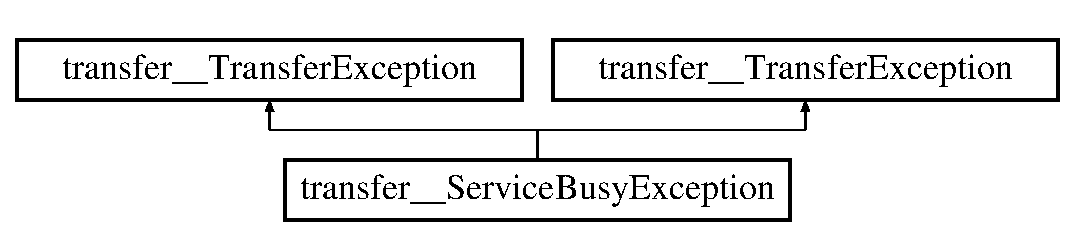
\includegraphics[height=2.000000cm]{classtransfer____ServiceBusyException}
\end{center}
\end{figure}
\subsection*{Public Member Functions}
\begin{DoxyCompactItemize}
\item 
virtual int {\bfseries soap\_\-type} () const \label{classtransfer____ServiceBusyException_ae66e53c6957d99516f54aa07f2304931}

\item 
virtual void {\bfseries soap\_\-default} (struct {\bf soap} $\ast$)\label{classtransfer____ServiceBusyException_a9f4ec5a0c05980001e6e2a7672056702}

\item 
virtual void {\bfseries soap\_\-serialize} (struct {\bf soap} $\ast$) const \label{classtransfer____ServiceBusyException_a2063b88ee61cf03513920ea37784bb27}

\item 
virtual int {\bfseries soap\_\-put} (struct {\bf soap} $\ast$, const char $\ast$, const char $\ast$) const \label{classtransfer____ServiceBusyException_a4f006f3ca3ace06b6a1b03ad14d5d2c3}

\item 
virtual int {\bfseries soap\_\-out} (struct {\bf soap} $\ast$, const char $\ast$, int, const char $\ast$) const \label{classtransfer____ServiceBusyException_aad3fd5a728829e0ca90e1b331cb0e2fa}

\item 
virtual void $\ast$ {\bfseries soap\_\-get} (struct {\bf soap} $\ast$, const char $\ast$, const char $\ast$)\label{classtransfer____ServiceBusyException_a5bbc44b85968a28d98120c23ee95e4d9}

\item 
virtual void $\ast$ {\bfseries soap\_\-in} (struct {\bf soap} $\ast$, const char $\ast$, const char $\ast$)\label{classtransfer____ServiceBusyException_afae8d05d864e9c4f01a30b7c45f9065e}

\end{DoxyCompactItemize}


\subsection{Detailed Description}
\char`\"{}http://transfer.data.glite.org\char`\"{}:ServiceBusyException is a complexType with complexContent extension of \char`\"{}http://transfer.data.glite.org\char`\"{}:TransferException. 

Definition at line 399 of file fts3-\/transfer-\/submit.h.



The documentation for this class was generated from the following files:\begin{DoxyCompactItemize}
\item 
src/CLI/fts3-\/transfer-\/submit.h\item 
src/CLI/ftsStub.h\item 
src/CLI/ftsC.cpp\end{DoxyCompactItemize}

\section{transfer\_\-\_\-StringPair Class Reference}
\label{classtransfer____StringPair}\index{transfer\_\-\_\-StringPair@{transfer\_\-\_\-StringPair}}


\char`\"{}http://transfer.data.glite.org\char`\"{}:StringPair is a complexType.  




{\ttfamily \#include $<$fts3-\/transfer-\/submit.h$>$}

\subsection*{Public Member Functions}
\begin{DoxyCompactItemize}
\item 
virtual int {\bfseries soap\_\-type} () const \label{classtransfer____StringPair_a9cd1e400332a0a45cec0229570dc36f7}

\item 
virtual void {\bfseries soap\_\-default} (struct {\bf soap} $\ast$)\label{classtransfer____StringPair_a7d34c028f43bcb89013da38ed91d2863}

\item 
virtual void {\bfseries soap\_\-serialize} (struct {\bf soap} $\ast$) const \label{classtransfer____StringPair_a8deebc2de84a4e7b692e87580d37864e}

\item 
virtual int {\bfseries soap\_\-put} (struct {\bf soap} $\ast$, const char $\ast$, const char $\ast$) const \label{classtransfer____StringPair_ae019859f493b0fb229d35bbac12fb544}

\item 
virtual int {\bfseries soap\_\-out} (struct {\bf soap} $\ast$, const char $\ast$, int, const char $\ast$) const \label{classtransfer____StringPair_ae491675d9ba8508dc8c3faefba5fef9d}

\item 
virtual void $\ast$ {\bfseries soap\_\-get} (struct {\bf soap} $\ast$, const char $\ast$, const char $\ast$)\label{classtransfer____StringPair_a3db494369b625f9d05f739b78897d9f5}

\item 
virtual void $\ast$ {\bfseries soap\_\-in} (struct {\bf soap} $\ast$, const char $\ast$, const char $\ast$)\label{classtransfer____StringPair_a25af095ae8bad4a7d2ca38f546e21c22}

\end{DoxyCompactItemize}
\subsection*{Data Fields}
\begin{DoxyCompactItemize}
\item 
std::string $\ast$ {\bf string1}
\begin{DoxyCompactList}\small\item\em Element string1 of type xs:string. \item\end{DoxyCompactList}\item 
std::string $\ast$ {\bf string2}
\begin{DoxyCompactList}\small\item\em Element string2 of type xs:string. \item\end{DoxyCompactList}\item 
struct {\bf soap} $\ast$ {\bf soap}\label{classtransfer____StringPair_a476511de19ad330c660dd803c0da2025}

\begin{DoxyCompactList}\small\item\em A handle to the soap struct that manages this instance (automatically set) \item\end{DoxyCompactList}\end{DoxyCompactItemize}


\subsection{Detailed Description}
\char`\"{}http://transfer.data.glite.org\char`\"{}:StringPair is a complexType. 

Definition at line 319 of file fts3-\/transfer-\/submit.h.



\subsection{Field Documentation}
\index{transfer\_\-\_\-StringPair@{transfer\_\-\_\-StringPair}!string1@{string1}}
\index{string1@{string1}!transfer__StringPair@{transfer\_\-\_\-StringPair}}
\subsubsection[{string1}]{\setlength{\rightskip}{0pt plus 5cm}std::string $\ast$ {\bf transfer\_\-\_\-StringPair::string1}}\label{classtransfer____StringPair_a007d23397bea7f93904fb80e81ab50a5}


Element string1 of type xs:string. 

Nullable pointer. 

Definition at line 322 of file fts3-\/transfer-\/submit.h.

\index{transfer\_\-\_\-StringPair@{transfer\_\-\_\-StringPair}!string2@{string2}}
\index{string2@{string2}!transfer__StringPair@{transfer\_\-\_\-StringPair}}
\subsubsection[{string2}]{\setlength{\rightskip}{0pt plus 5cm}std::string $\ast$ {\bf transfer\_\-\_\-StringPair::string2}}\label{classtransfer____StringPair_a2aa408d34b32e657c4f5bbdddb862814}


Element string2 of type xs:string. 

Nullable pointer. 

Definition at line 324 of file fts3-\/transfer-\/submit.h.



The documentation for this class was generated from the following files:\begin{DoxyCompactItemize}
\item 
src/CLI/fts3-\/transfer-\/submit.h\item 
src/CLI/ftsStub.h\item 
src/CLI/ftsC.cpp\end{DoxyCompactItemize}

\section{transfer\_\-\_\-TransferException Class Reference}
\label{classtransfer____TransferException}\index{transfer\_\-\_\-TransferException@{transfer\_\-\_\-TransferException}}


\char`\"{}http://transfer.data.glite.org\char`\"{}:TransferException is a complexType.  




{\ttfamily \#include $<$fts3-\/transfer-\/submit.h$>$}

Inheritance diagram for transfer\_\-\_\-TransferException:\begin{figure}[H]
\begin{center}
\leavevmode
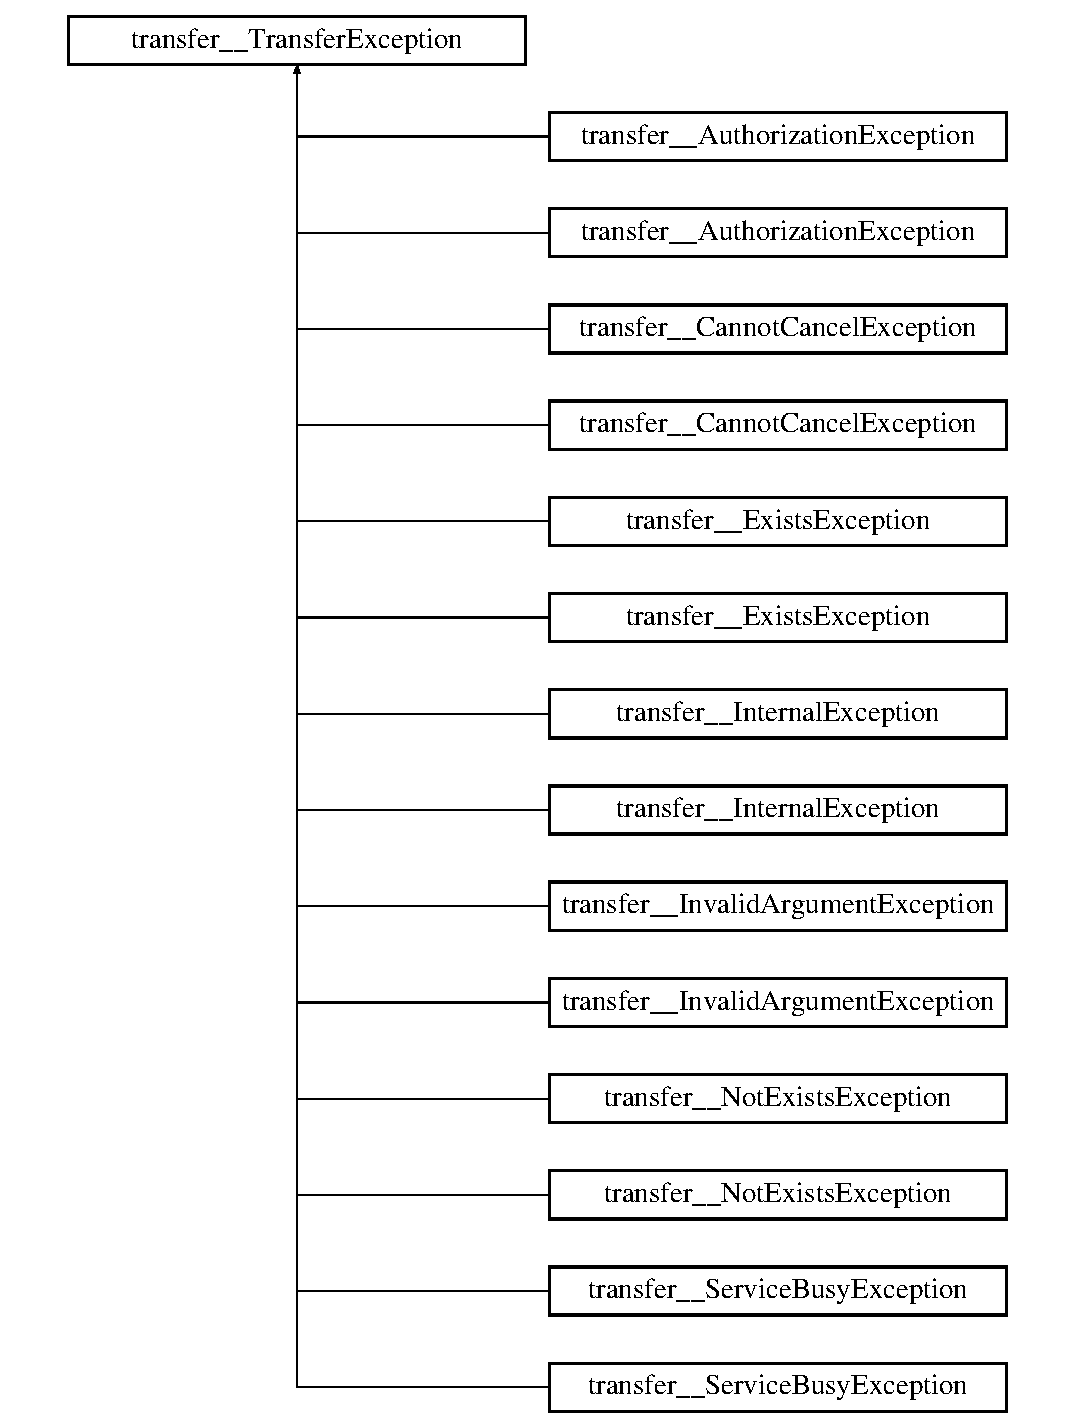
\includegraphics[height=12.000000cm]{classtransfer____TransferException}
\end{center}
\end{figure}
\subsection*{Public Member Functions}
\begin{DoxyCompactItemize}
\item 
virtual int {\bfseries soap\_\-type} () const \label{classtransfer____TransferException_ada3774e051f2702ea4ef9434a411ac3a}

\item 
virtual void {\bfseries soap\_\-default} (struct {\bf soap} $\ast$)\label{classtransfer____TransferException_afdd7f3fc6f29d1dff82ae4e0106a70b3}

\item 
virtual void {\bfseries soap\_\-serialize} (struct {\bf soap} $\ast$) const \label{classtransfer____TransferException_a5e2fe20a5322406aa67613a34df3d465}

\item 
virtual int {\bfseries soap\_\-put} (struct {\bf soap} $\ast$, const char $\ast$, const char $\ast$) const \label{classtransfer____TransferException_a238c3881c3d2d21f720251015dd215a2}

\item 
virtual int {\bfseries soap\_\-out} (struct {\bf soap} $\ast$, const char $\ast$, int, const char $\ast$) const \label{classtransfer____TransferException_a90076fe6913f429688bdab161422e464}

\item 
virtual void $\ast$ {\bfseries soap\_\-get} (struct {\bf soap} $\ast$, const char $\ast$, const char $\ast$)\label{classtransfer____TransferException_a39a79a991cccec1ebd6b07d58aaf5dc4}

\item 
virtual void $\ast$ {\bfseries soap\_\-in} (struct {\bf soap} $\ast$, const char $\ast$, const char $\ast$)\label{classtransfer____TransferException_a9e5d42911f2b8455de991d16ba4294fe}

\end{DoxyCompactItemize}
\subsection*{Data Fields}
\begin{DoxyCompactItemize}
\item 
std::string $\ast$ {\bf message}
\begin{DoxyCompactList}\small\item\em Element message of type xs:string. \item\end{DoxyCompactList}\item 
struct {\bf soap} $\ast$ {\bf soap}\label{classtransfer____TransferException_adcfb27ab8b2b611134e14c45825c89d2}

\begin{DoxyCompactList}\small\item\em A handle to the soap struct that manages this instance (automatically set) \item\end{DoxyCompactList}\end{DoxyCompactItemize}


\subsection{Detailed Description}
\char`\"{}http://transfer.data.glite.org\char`\"{}:TransferException is a complexType. 

Definition at line 181 of file fts3-\/transfer-\/submit.h.



\subsection{Field Documentation}
\index{transfer\_\-\_\-TransferException@{transfer\_\-\_\-TransferException}!message@{message}}
\index{message@{message}!transfer__TransferException@{transfer\_\-\_\-TransferException}}
\subsubsection[{message}]{\setlength{\rightskip}{0pt plus 5cm}std::string $\ast$ {\bf transfer\_\-\_\-TransferException::message}}\label{classtransfer____TransferException_ab7d44de4ff3d40739362d125663eeb09}


Element message of type xs:string. 

Nullable pointer. 

Definition at line 184 of file fts3-\/transfer-\/submit.h.



The documentation for this class was generated from the following files:\begin{DoxyCompactItemize}
\item 
src/CLI/fts3-\/transfer-\/submit.h\item 
src/CLI/ftsStub.h\item 
src/CLI/ftsC.cpp\end{DoxyCompactItemize}

\section{transfer\_\-\_\-TransferJob Class Reference}
\label{classtransfer____TransferJob}\index{transfer\_\-\_\-TransferJob@{transfer\_\-\_\-TransferJob}}


\char`\"{}http://transfer.data.glite.org\char`\"{}:TransferJob is a complexType.  




{\ttfamily \#include $<$fts3-\/transfer-\/submit.h$>$}

\subsection*{Public Member Functions}
\begin{DoxyCompactItemize}
\item 
virtual int {\bfseries soap\_\-type} () const \label{classtransfer____TransferJob_a435d142b7c18238e1efb3f1e2553c7e5}

\item 
virtual void {\bfseries soap\_\-default} (struct {\bf soap} $\ast$)\label{classtransfer____TransferJob_a709cdcf0f5ac21e219020f72aa2498a8}

\item 
virtual void {\bfseries soap\_\-serialize} (struct {\bf soap} $\ast$) const \label{classtransfer____TransferJob_ab0d8968ea31382f572e017870ba77234}

\item 
virtual int {\bfseries soap\_\-put} (struct {\bf soap} $\ast$, const char $\ast$, const char $\ast$) const \label{classtransfer____TransferJob_aee1881a31b62fc13e8461379c980a50f}

\item 
virtual int {\bfseries soap\_\-out} (struct {\bf soap} $\ast$, const char $\ast$, int, const char $\ast$) const \label{classtransfer____TransferJob_af95447f3ca57713e4d4aebc2e97c1453}

\item 
virtual void $\ast$ {\bfseries soap\_\-get} (struct {\bf soap} $\ast$, const char $\ast$, const char $\ast$)\label{classtransfer____TransferJob_add525c689a6052cd88ccdaa60f18ce80}

\item 
virtual void $\ast$ {\bfseries soap\_\-in} (struct {\bf soap} $\ast$, const char $\ast$, const char $\ast$)\label{classtransfer____TransferJob_ad4e215786c4388bc92d129d593e73c08}

\end{DoxyCompactItemize}
\subsection*{Data Fields}
\begin{DoxyCompactItemize}
\item 
std::vector$<$ {\bf transfer\_\-\_\-TransferJobElement} $\ast$ $>$ {\bf transferJobElements}
\begin{DoxyCompactList}\small\item\em Vector of transfer\_\-\_\-TransferJobElement$\ast$ with length 1..unbounded. \item\end{DoxyCompactList}\item 
{\bf transfer\_\-\_\-TransferParams} $\ast$ {\bf jobParams}
\begin{DoxyCompactList}\small\item\em Element jobParams of type \char`\"{}http://transfer.data.glite.org\char`\"{}:TransferParams. \item\end{DoxyCompactList}\item 
std::string $\ast$ {\bf credential}
\begin{DoxyCompactList}\small\item\em Element credential of type xs:string. \item\end{DoxyCompactList}\item 
struct {\bf soap} $\ast$ {\bf soap}\label{classtransfer____TransferJob_a8e3bac28f1271ff47a846ca122de51c7}

\begin{DoxyCompactList}\small\item\em A handle to the soap struct that manages this instance (automatically set) \item\end{DoxyCompactList}\end{DoxyCompactItemize}


\subsection{Detailed Description}
\char`\"{}http://transfer.data.glite.org\char`\"{}:TransferJob is a complexType. 

Definition at line 201 of file fts3-\/transfer-\/submit.h.



\subsection{Field Documentation}
\index{transfer\_\-\_\-TransferJob@{transfer\_\-\_\-TransferJob}!credential@{credential}}
\index{credential@{credential}!transfer__TransferJob@{transfer\_\-\_\-TransferJob}}
\subsubsection[{credential}]{\setlength{\rightskip}{0pt plus 5cm}std::string $\ast$ {\bf transfer\_\-\_\-TransferJob::credential}}\label{classtransfer____TransferJob_a75ed6de04bbb682618911ba8c21d3010}


Element credential of type xs:string. 

Nullable pointer. 

Definition at line 208 of file fts3-\/transfer-\/submit.h.

\index{transfer\_\-\_\-TransferJob@{transfer\_\-\_\-TransferJob}!jobParams@{jobParams}}
\index{jobParams@{jobParams}!transfer__TransferJob@{transfer\_\-\_\-TransferJob}}
\subsubsection[{jobParams}]{\setlength{\rightskip}{0pt plus 5cm}{\bf transfer\_\-\_\-TransferParams} $\ast$ {\bf transfer\_\-\_\-TransferJob::jobParams}}\label{classtransfer____TransferJob_acb79bfcb008745f36e641c5e5a9a5abb}


Element jobParams of type \char`\"{}http://transfer.data.glite.org\char`\"{}:TransferParams. 

Nullable pointer. 

Definition at line 206 of file fts3-\/transfer-\/submit.h.

\index{transfer\_\-\_\-TransferJob@{transfer\_\-\_\-TransferJob}!transferJobElements@{transferJobElements}}
\index{transferJobElements@{transferJobElements}!transfer__TransferJob@{transfer\_\-\_\-TransferJob}}
\subsubsection[{transferJobElements}]{\setlength{\rightskip}{0pt plus 5cm}std::vector$<$ {\bf transfer\_\-\_\-TransferJobElement} $\ast$ $>$ {\bf transfer\_\-\_\-TransferJob::transferJobElements}}\label{classtransfer____TransferJob_acff3d8c546e3134bcd42cdf81a1e5357}


Vector of transfer\_\-\_\-TransferJobElement$\ast$ with length 1..unbounded. 

Nullable pointer. 

Definition at line 204 of file fts3-\/transfer-\/submit.h.



The documentation for this class was generated from the following files:\begin{DoxyCompactItemize}
\item 
src/CLI/fts3-\/transfer-\/submit.h\item 
src/CLI/ftsStub.h\item 
src/CLI/ftsC.cpp\end{DoxyCompactItemize}

\section{transfer\_\-\_\-TransferJob2 Class Reference}
\label{classtransfer____TransferJob2}\index{transfer\_\-\_\-TransferJob2@{transfer\_\-\_\-TransferJob2}}


\char`\"{}http://transfer.data.glite.org\char`\"{}:TransferJob2 is a complexType.  




{\ttfamily \#include $<$fts3-\/transfer-\/submit.h$>$}

\subsection*{Public Member Functions}
\begin{DoxyCompactItemize}
\item 
virtual int {\bfseries soap\_\-type} () const \label{classtransfer____TransferJob2_a6f5b4aa33457e66ab9025d099e723096}

\item 
virtual void {\bfseries soap\_\-default} (struct {\bf soap} $\ast$)\label{classtransfer____TransferJob2_aacf858392122a8abf7f0df46c302c2cc}

\item 
virtual void {\bfseries soap\_\-serialize} (struct {\bf soap} $\ast$) const \label{classtransfer____TransferJob2_a9c10cc00f42ceecdd4d0fb4b8d7416f9}

\item 
virtual int {\bfseries soap\_\-put} (struct {\bf soap} $\ast$, const char $\ast$, const char $\ast$) const \label{classtransfer____TransferJob2_aa413088ea904a64134c77d5fc16b432a}

\item 
virtual int {\bfseries soap\_\-out} (struct {\bf soap} $\ast$, const char $\ast$, int, const char $\ast$) const \label{classtransfer____TransferJob2_a0d9f041e802b1dad61e406733c63ac53}

\item 
virtual void $\ast$ {\bfseries soap\_\-get} (struct {\bf soap} $\ast$, const char $\ast$, const char $\ast$)\label{classtransfer____TransferJob2_a7a0249083583867b341d8ff46fcc0da8}

\item 
virtual void $\ast$ {\bfseries soap\_\-in} (struct {\bf soap} $\ast$, const char $\ast$, const char $\ast$)\label{classtransfer____TransferJob2_a8eac1aa3fa0e5a7cf3823175ced31e07}

\end{DoxyCompactItemize}
\subsection*{Data Fields}
\begin{DoxyCompactItemize}
\item 
std::vector$<$ {\bf transfer\_\-\_\-TransferJobElement2} $\ast$ $>$ {\bf transferJobElements}
\begin{DoxyCompactList}\small\item\em Vector of transfer\_\-\_\-TransferJobElement2$\ast$ with length 1..unbounded. \item\end{DoxyCompactList}\item 
{\bf transfer\_\-\_\-TransferParams} $\ast$ {\bf jobParams}
\begin{DoxyCompactList}\small\item\em Element jobParams of type \char`\"{}http://transfer.data.glite.org\char`\"{}:TransferParams. \item\end{DoxyCompactList}\item 
std::string $\ast$ {\bf credential}
\begin{DoxyCompactList}\small\item\em Element credential of type xs:string. \item\end{DoxyCompactList}\item 
struct {\bf soap} $\ast$ {\bf soap}\label{classtransfer____TransferJob2_a17b51b9c1a0eb5dbca504d5003321107}

\begin{DoxyCompactList}\small\item\em A handle to the soap struct that manages this instance (automatically set) \item\end{DoxyCompactList}\end{DoxyCompactItemize}


\subsection{Detailed Description}
\char`\"{}http://transfer.data.glite.org\char`\"{}:TransferJob2 is a complexType. 

Definition at line 227 of file fts3-\/transfer-\/submit.h.



\subsection{Field Documentation}
\index{transfer\_\-\_\-TransferJob2@{transfer\_\-\_\-TransferJob2}!credential@{credential}}
\index{credential@{credential}!transfer__TransferJob2@{transfer\_\-\_\-TransferJob2}}
\subsubsection[{credential}]{\setlength{\rightskip}{0pt plus 5cm}std::string $\ast$ {\bf transfer\_\-\_\-TransferJob2::credential}}\label{classtransfer____TransferJob2_ada735715456be6ed04899f941cc9b11a}


Element credential of type xs:string. 

Nullable pointer. 

Definition at line 234 of file fts3-\/transfer-\/submit.h.

\index{transfer\_\-\_\-TransferJob2@{transfer\_\-\_\-TransferJob2}!jobParams@{jobParams}}
\index{jobParams@{jobParams}!transfer__TransferJob2@{transfer\_\-\_\-TransferJob2}}
\subsubsection[{jobParams}]{\setlength{\rightskip}{0pt plus 5cm}{\bf transfer\_\-\_\-TransferParams} $\ast$ {\bf transfer\_\-\_\-TransferJob2::jobParams}}\label{classtransfer____TransferJob2_a4897231653618589fd9362969298a494}


Element jobParams of type \char`\"{}http://transfer.data.glite.org\char`\"{}:TransferParams. 

Nullable pointer. 

Definition at line 232 of file fts3-\/transfer-\/submit.h.

\index{transfer\_\-\_\-TransferJob2@{transfer\_\-\_\-TransferJob2}!transferJobElements@{transferJobElements}}
\index{transferJobElements@{transferJobElements}!transfer__TransferJob2@{transfer\_\-\_\-TransferJob2}}
\subsubsection[{transferJobElements}]{\setlength{\rightskip}{0pt plus 5cm}std::vector$<$ {\bf transfer\_\-\_\-TransferJobElement2} $\ast$ $>$ {\bf transfer\_\-\_\-TransferJob2::transferJobElements}}\label{classtransfer____TransferJob2_a092c850c457a62e8850699d72b810104}


Vector of transfer\_\-\_\-TransferJobElement2$\ast$ with length 1..unbounded. 

Nullable pointer. 

Definition at line 230 of file fts3-\/transfer-\/submit.h.



The documentation for this class was generated from the following files:\begin{DoxyCompactItemize}
\item 
src/CLI/fts3-\/transfer-\/submit.h\item 
src/CLI/ftsStub.h\item 
src/CLI/ftsC.cpp\end{DoxyCompactItemize}

\section{transfer\_\-\_\-TransferJobElement Class Reference}
\label{classtransfer____TransferJobElement}\index{transfer\_\-\_\-TransferJobElement@{transfer\_\-\_\-TransferJobElement}}


\char`\"{}http://transfer.data.glite.org\char`\"{}:TransferJobElement is a complexType.  




{\ttfamily \#include $<$fts3-\/transfer-\/submit.h$>$}

\subsection*{Public Member Functions}
\begin{DoxyCompactItemize}
\item 
virtual int {\bfseries soap\_\-type} () const \label{classtransfer____TransferJobElement_aabd7d06ef5e049122f207607d1815048}

\item 
virtual void {\bfseries soap\_\-default} (struct {\bf soap} $\ast$)\label{classtransfer____TransferJobElement_acca82e2a7d135705dbd2f2599bfa4a6d}

\item 
virtual void {\bfseries soap\_\-serialize} (struct {\bf soap} $\ast$) const \label{classtransfer____TransferJobElement_ac64c93da6a0bc5c8b194208d1911cdd0}

\item 
virtual int {\bfseries soap\_\-put} (struct {\bf soap} $\ast$, const char $\ast$, const char $\ast$) const \label{classtransfer____TransferJobElement_ae9c11deaf7ab43f4a5f45a542b0d8f8d}

\item 
virtual int {\bfseries soap\_\-out} (struct {\bf soap} $\ast$, const char $\ast$, int, const char $\ast$) const \label{classtransfer____TransferJobElement_aea76fb30df6904dcc6142550622efed7}

\item 
virtual void $\ast$ {\bfseries soap\_\-get} (struct {\bf soap} $\ast$, const char $\ast$, const char $\ast$)\label{classtransfer____TransferJobElement_a22d2f480e751707d8a64efd768eabea4}

\item 
virtual void $\ast$ {\bfseries soap\_\-in} (struct {\bf soap} $\ast$, const char $\ast$, const char $\ast$)\label{classtransfer____TransferJobElement_a966e5798fc9acc069d5723da0b75ed4d}

\end{DoxyCompactItemize}
\subsection*{Data Fields}
\begin{DoxyCompactItemize}
\item 
std::string $\ast$ {\bf source}
\begin{DoxyCompactList}\small\item\em Element source of type xs:string. \item\end{DoxyCompactList}\item 
std::string $\ast$ {\bf dest}
\begin{DoxyCompactList}\small\item\em Element dest of type xs:string. \item\end{DoxyCompactList}\item 
struct {\bf soap} $\ast$ {\bf soap}\label{classtransfer____TransferJobElement_a6d4439616ecd6bcee00929a501572abd}

\begin{DoxyCompactList}\small\item\em A handle to the soap struct that manages this instance (automatically set) \item\end{DoxyCompactList}\end{DoxyCompactItemize}


\subsection{Detailed Description}
\char`\"{}http://transfer.data.glite.org\char`\"{}:TransferJobElement is a complexType. 

Definition at line 190 of file fts3-\/transfer-\/submit.h.



\subsection{Field Documentation}
\index{transfer\_\-\_\-TransferJobElement@{transfer\_\-\_\-TransferJobElement}!dest@{dest}}
\index{dest@{dest}!transfer__TransferJobElement@{transfer\_\-\_\-TransferJobElement}}
\subsubsection[{dest}]{\setlength{\rightskip}{0pt plus 5cm}std::string $\ast$ {\bf transfer\_\-\_\-TransferJobElement::dest}}\label{classtransfer____TransferJobElement_aa6ad4c72af630c766d440187a81f8f68}


Element dest of type xs:string. 

Nullable pointer. 

Definition at line 195 of file fts3-\/transfer-\/submit.h.

\index{transfer\_\-\_\-TransferJobElement@{transfer\_\-\_\-TransferJobElement}!source@{source}}
\index{source@{source}!transfer__TransferJobElement@{transfer\_\-\_\-TransferJobElement}}
\subsubsection[{source}]{\setlength{\rightskip}{0pt plus 5cm}std::string $\ast$ {\bf transfer\_\-\_\-TransferJobElement::source}}\label{classtransfer____TransferJobElement_a705f3b30aa519c3f9f7ceca37c9120c0}


Element source of type xs:string. 

Nullable pointer. 

Definition at line 193 of file fts3-\/transfer-\/submit.h.



The documentation for this class was generated from the following files:\begin{DoxyCompactItemize}
\item 
src/CLI/fts3-\/transfer-\/submit.h\item 
src/CLI/ftsStub.h\item 
src/CLI/ftsC.cpp\end{DoxyCompactItemize}

\section{transfer\_\-\_\-TransferJobElement2 Class Reference}
\label{classtransfer____TransferJobElement2}\index{transfer\_\-\_\-TransferJobElement2@{transfer\_\-\_\-TransferJobElement2}}


\char`\"{}http://transfer.data.glite.org\char`\"{}:TransferJobElement2 is a complexType.  




{\ttfamily \#include $<$fts3-\/transfer-\/submit.h$>$}

\subsection*{Public Member Functions}
\begin{DoxyCompactItemize}
\item 
virtual int {\bfseries soap\_\-type} () const \label{classtransfer____TransferJobElement2_a77faf0214629f9949c7e11b8e72cc278}

\item 
virtual void {\bfseries soap\_\-default} (struct {\bf soap} $\ast$)\label{classtransfer____TransferJobElement2_a2ee361c3004e9761da2e2a4bedd842b6}

\item 
virtual void {\bfseries soap\_\-serialize} (struct {\bf soap} $\ast$) const \label{classtransfer____TransferJobElement2_abf0c019c9ab22f3086f00c14adac9b26}

\item 
virtual int {\bfseries soap\_\-put} (struct {\bf soap} $\ast$, const char $\ast$, const char $\ast$) const \label{classtransfer____TransferJobElement2_a04d8d08eaf15b2bb01ed2c5d79a709fd}

\item 
virtual int {\bfseries soap\_\-out} (struct {\bf soap} $\ast$, const char $\ast$, int, const char $\ast$) const \label{classtransfer____TransferJobElement2_a457c25419762ac72252a9315eea934a7}

\item 
virtual void $\ast$ {\bfseries soap\_\-get} (struct {\bf soap} $\ast$, const char $\ast$, const char $\ast$)\label{classtransfer____TransferJobElement2_a4cbab712b1ccae7f45bb652c86b6b80f}

\item 
virtual void $\ast$ {\bfseries soap\_\-in} (struct {\bf soap} $\ast$, const char $\ast$, const char $\ast$)\label{classtransfer____TransferJobElement2_ae53dcbc7ed7f19c99afe80b1a2d6830d}

\end{DoxyCompactItemize}
\subsection*{Data Fields}
\begin{DoxyCompactItemize}
\item 
std::string $\ast$ {\bf source}
\begin{DoxyCompactList}\small\item\em Element source of type xs:string. \item\end{DoxyCompactList}\item 
std::string $\ast$ {\bf dest}
\begin{DoxyCompactList}\small\item\em Element dest of type xs:string. \item\end{DoxyCompactList}\item 
std::string $\ast$ {\bf checksum}
\begin{DoxyCompactList}\small\item\em Element checksum of type xs:string. \item\end{DoxyCompactList}\item 
struct {\bf soap} $\ast$ {\bf soap}\label{classtransfer____TransferJobElement2_a8b8db45a0818659cc38ebeaae606ce65}

\begin{DoxyCompactList}\small\item\em A handle to the soap struct that manages this instance (automatically set) \item\end{DoxyCompactList}\end{DoxyCompactItemize}


\subsection{Detailed Description}
\char`\"{}http://transfer.data.glite.org\char`\"{}:TransferJobElement2 is a complexType. 

Definition at line 214 of file fts3-\/transfer-\/submit.h.



\subsection{Field Documentation}
\index{transfer\_\-\_\-TransferJobElement2@{transfer\_\-\_\-TransferJobElement2}!checksum@{checksum}}
\index{checksum@{checksum}!transfer__TransferJobElement2@{transfer\_\-\_\-TransferJobElement2}}
\subsubsection[{checksum}]{\setlength{\rightskip}{0pt plus 5cm}std::string $\ast$ {\bf transfer\_\-\_\-TransferJobElement2::checksum}}\label{classtransfer____TransferJobElement2_a0a1f9ef5e139f3b425f50a37a1022118}


Element checksum of type xs:string. 

Nullable pointer. 

Definition at line 221 of file fts3-\/transfer-\/submit.h.

\index{transfer\_\-\_\-TransferJobElement2@{transfer\_\-\_\-TransferJobElement2}!dest@{dest}}
\index{dest@{dest}!transfer__TransferJobElement2@{transfer\_\-\_\-TransferJobElement2}}
\subsubsection[{dest}]{\setlength{\rightskip}{0pt plus 5cm}std::string $\ast$ {\bf transfer\_\-\_\-TransferJobElement2::dest}}\label{classtransfer____TransferJobElement2_a6c50f9c4b0c2a6394c4004bb486355e5}


Element dest of type xs:string. 

Nullable pointer. 

Definition at line 219 of file fts3-\/transfer-\/submit.h.

\index{transfer\_\-\_\-TransferJobElement2@{transfer\_\-\_\-TransferJobElement2}!source@{source}}
\index{source@{source}!transfer__TransferJobElement2@{transfer\_\-\_\-TransferJobElement2}}
\subsubsection[{source}]{\setlength{\rightskip}{0pt plus 5cm}std::string $\ast$ {\bf transfer\_\-\_\-TransferJobElement2::source}}\label{classtransfer____TransferJobElement2_aac5f816bc5bf77fe3e33348a4cfb16db}


Element source of type xs:string. 

Nullable pointer. 

Definition at line 217 of file fts3-\/transfer-\/submit.h.



The documentation for this class was generated from the following files:\begin{DoxyCompactItemize}
\item 
src/CLI/fts3-\/transfer-\/submit.h\item 
src/CLI/ftsStub.h\item 
src/CLI/ftsC.cpp\end{DoxyCompactItemize}

\section{transfer\_\-\_\-TransferJobSummary Class Reference}
\label{classtransfer____TransferJobSummary}\index{transfer\_\-\_\-TransferJobSummary@{transfer\_\-\_\-TransferJobSummary}}


\char`\"{}http://transfer.data.glite.org\char`\"{}:TransferJobSummary is a complexType.  




{\ttfamily \#include $<$fts3-\/transfer-\/submit.h$>$}

Inheritance diagram for transfer\_\-\_\-TransferJobSummary:\begin{figure}[H]
\begin{center}
\leavevmode
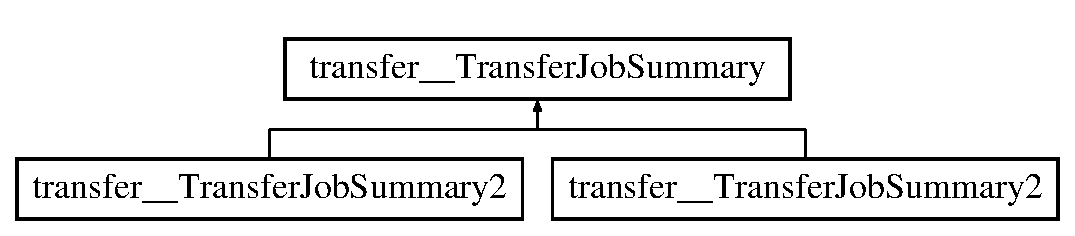
\includegraphics[height=2.000000cm]{classtransfer____TransferJobSummary}
\end{center}
\end{figure}
\subsection*{Public Member Functions}
\begin{DoxyCompactItemize}
\item 
virtual int {\bfseries soap\_\-type} () const \label{classtransfer____TransferJobSummary_a2f8087d179233d73e8bfe981102be26d}

\item 
virtual void {\bfseries soap\_\-default} (struct {\bf soap} $\ast$)\label{classtransfer____TransferJobSummary_a34c4825f129ed7b43e30a415bde880be}

\item 
virtual void {\bfseries soap\_\-serialize} (struct {\bf soap} $\ast$) const \label{classtransfer____TransferJobSummary_a0e2c17378ba0c34ba5b252489010be65}

\item 
virtual int {\bfseries soap\_\-put} (struct {\bf soap} $\ast$, const char $\ast$, const char $\ast$) const \label{classtransfer____TransferJobSummary_a6b0dfa6e1e0d7287aa1928576f3e5a44}

\item 
virtual int {\bfseries soap\_\-out} (struct {\bf soap} $\ast$, const char $\ast$, int, const char $\ast$) const \label{classtransfer____TransferJobSummary_a3041041bbe2df7e15ce159d144c2b133}

\item 
virtual void $\ast$ {\bfseries soap\_\-get} (struct {\bf soap} $\ast$, const char $\ast$, const char $\ast$)\label{classtransfer____TransferJobSummary_afe19deb1a2e3c1ac3d41b6680f9025d7}

\item 
virtual void $\ast$ {\bfseries soap\_\-in} (struct {\bf soap} $\ast$, const char $\ast$, const char $\ast$)\label{classtransfer____TransferJobSummary_ad8c54d84b5f57f05936a6626f9941257}

\end{DoxyCompactItemize}
\subsection*{Data Fields}
\begin{DoxyCompactItemize}
\item 
{\bf transfer\_\-\_\-JobStatus} $\ast$ {\bf jobStatus}
\begin{DoxyCompactList}\small\item\em Element jobStatus of type \char`\"{}http://transfer.data.glite.org\char`\"{}:JobStatus. \item\end{DoxyCompactList}\item 
int {\bf numDone}
\begin{DoxyCompactList}\small\item\em Element numDone of type xs:int. \item\end{DoxyCompactList}\item 
int {\bf numActive}
\begin{DoxyCompactList}\small\item\em Element numActive of type xs:int. \item\end{DoxyCompactList}\item 
int {\bf numPending}
\begin{DoxyCompactList}\small\item\em Element numPending of type xs:int. \item\end{DoxyCompactList}\item 
int {\bf numCanceled}
\begin{DoxyCompactList}\small\item\em Element numCanceled of type xs:int. \item\end{DoxyCompactList}\item 
int {\bf numCanceling}
\begin{DoxyCompactList}\small\item\em Element numCanceling of type xs:int. \item\end{DoxyCompactList}\item 
int {\bf numFailed}
\begin{DoxyCompactList}\small\item\em Element numFailed of type xs:int. \item\end{DoxyCompactList}\item 
int {\bf numFinished}
\begin{DoxyCompactList}\small\item\em Element numFinished of type xs:int. \item\end{DoxyCompactList}\item 
int {\bf numSubmitted}
\begin{DoxyCompactList}\small\item\em Element numSubmitted of type xs:int. \item\end{DoxyCompactList}\item 
int {\bf numHold}
\begin{DoxyCompactList}\small\item\em Element numHold of type xs:int. \item\end{DoxyCompactList}\item 
int {\bf numWaiting}
\begin{DoxyCompactList}\small\item\em Element numWaiting of type xs:int. \item\end{DoxyCompactList}\item 
int {\bf numCatalogFailed}
\begin{DoxyCompactList}\small\item\em Element numCatalogFailed of type xs:int. \item\end{DoxyCompactList}\item 
int {\bf numRestarted}
\begin{DoxyCompactList}\small\item\em Element numRestarted of type xs:int. \item\end{DoxyCompactList}\item 
struct {\bf soap} $\ast$ {\bf soap}\label{classtransfer____TransferJobSummary_a799d3324a2cc9a8bcd8a1c9442eec31d}

\begin{DoxyCompactList}\small\item\em A handle to the soap struct that manages this instance (automatically set) \item\end{DoxyCompactList}\end{DoxyCompactItemize}


\subsection{Detailed Description}
\char`\"{}http://transfer.data.glite.org\char`\"{}:TransferJobSummary is a complexType. 

Definition at line 286 of file fts3-\/transfer-\/submit.h.



\subsection{Field Documentation}
\index{transfer\_\-\_\-TransferJobSummary@{transfer\_\-\_\-TransferJobSummary}!jobStatus@{jobStatus}}
\index{jobStatus@{jobStatus}!transfer__TransferJobSummary@{transfer\_\-\_\-TransferJobSummary}}
\subsubsection[{jobStatus}]{\setlength{\rightskip}{0pt plus 5cm}{\bf transfer\_\-\_\-JobStatus} $\ast$ {\bf transfer\_\-\_\-TransferJobSummary::jobStatus}}\label{classtransfer____TransferJobSummary_ac3a623ce12953dc1b8bc55bde5661e9d}


Element jobStatus of type \char`\"{}http://transfer.data.glite.org\char`\"{}:JobStatus. 

Nullable pointer. 

Definition at line 289 of file fts3-\/transfer-\/submit.h.

\index{transfer\_\-\_\-TransferJobSummary@{transfer\_\-\_\-TransferJobSummary}!numActive@{numActive}}
\index{numActive@{numActive}!transfer__TransferJobSummary@{transfer\_\-\_\-TransferJobSummary}}
\subsubsection[{numActive}]{\setlength{\rightskip}{0pt plus 5cm}int {\bf transfer\_\-\_\-TransferJobSummary::numActive}}\label{classtransfer____TransferJobSummary_abad0632f4ab1ce47be933c8b8427f047}


Element numActive of type xs:int. 

Required element. 

Definition at line 293 of file fts3-\/transfer-\/submit.h.

\index{transfer\_\-\_\-TransferJobSummary@{transfer\_\-\_\-TransferJobSummary}!numCanceled@{numCanceled}}
\index{numCanceled@{numCanceled}!transfer__TransferJobSummary@{transfer\_\-\_\-TransferJobSummary}}
\subsubsection[{numCanceled}]{\setlength{\rightskip}{0pt plus 5cm}int {\bf transfer\_\-\_\-TransferJobSummary::numCanceled}}\label{classtransfer____TransferJobSummary_a1a213ed80c66cc147369d3f63fa8cb28}


Element numCanceled of type xs:int. 

Required element. 

Definition at line 297 of file fts3-\/transfer-\/submit.h.

\index{transfer\_\-\_\-TransferJobSummary@{transfer\_\-\_\-TransferJobSummary}!numCanceling@{numCanceling}}
\index{numCanceling@{numCanceling}!transfer__TransferJobSummary@{transfer\_\-\_\-TransferJobSummary}}
\subsubsection[{numCanceling}]{\setlength{\rightskip}{0pt plus 5cm}int {\bf transfer\_\-\_\-TransferJobSummary::numCanceling}}\label{classtransfer____TransferJobSummary_ae95e634dad337feb60311f67bf072160}


Element numCanceling of type xs:int. 

Required element. 

Definition at line 299 of file fts3-\/transfer-\/submit.h.

\index{transfer\_\-\_\-TransferJobSummary@{transfer\_\-\_\-TransferJobSummary}!numCatalogFailed@{numCatalogFailed}}
\index{numCatalogFailed@{numCatalogFailed}!transfer__TransferJobSummary@{transfer\_\-\_\-TransferJobSummary}}
\subsubsection[{numCatalogFailed}]{\setlength{\rightskip}{0pt plus 5cm}int {\bf transfer\_\-\_\-TransferJobSummary::numCatalogFailed}}\label{classtransfer____TransferJobSummary_ae9fd48b3db1b975868c370df4015adef}


Element numCatalogFailed of type xs:int. 

Required element. 

Definition at line 311 of file fts3-\/transfer-\/submit.h.

\index{transfer\_\-\_\-TransferJobSummary@{transfer\_\-\_\-TransferJobSummary}!numDone@{numDone}}
\index{numDone@{numDone}!transfer__TransferJobSummary@{transfer\_\-\_\-TransferJobSummary}}
\subsubsection[{numDone}]{\setlength{\rightskip}{0pt plus 5cm}int {\bf transfer\_\-\_\-TransferJobSummary::numDone}}\label{classtransfer____TransferJobSummary_af4ce403c9dd716b34b33fa048038317a}


Element numDone of type xs:int. 

Required element. 

Definition at line 291 of file fts3-\/transfer-\/submit.h.

\index{transfer\_\-\_\-TransferJobSummary@{transfer\_\-\_\-TransferJobSummary}!numFailed@{numFailed}}
\index{numFailed@{numFailed}!transfer__TransferJobSummary@{transfer\_\-\_\-TransferJobSummary}}
\subsubsection[{numFailed}]{\setlength{\rightskip}{0pt plus 5cm}int {\bf transfer\_\-\_\-TransferJobSummary::numFailed}}\label{classtransfer____TransferJobSummary_ad694259cb44aa87f1518b6ffb97bff0f}


Element numFailed of type xs:int. 

Required element. 

Definition at line 301 of file fts3-\/transfer-\/submit.h.

\index{transfer\_\-\_\-TransferJobSummary@{transfer\_\-\_\-TransferJobSummary}!numFinished@{numFinished}}
\index{numFinished@{numFinished}!transfer__TransferJobSummary@{transfer\_\-\_\-TransferJobSummary}}
\subsubsection[{numFinished}]{\setlength{\rightskip}{0pt plus 5cm}int {\bf transfer\_\-\_\-TransferJobSummary::numFinished}}\label{classtransfer____TransferJobSummary_ae47631ae2f0542e8339e33f6b8403d3a}


Element numFinished of type xs:int. 

Required element. 

Definition at line 303 of file fts3-\/transfer-\/submit.h.

\index{transfer\_\-\_\-TransferJobSummary@{transfer\_\-\_\-TransferJobSummary}!numHold@{numHold}}
\index{numHold@{numHold}!transfer__TransferJobSummary@{transfer\_\-\_\-TransferJobSummary}}
\subsubsection[{numHold}]{\setlength{\rightskip}{0pt plus 5cm}int {\bf transfer\_\-\_\-TransferJobSummary::numHold}}\label{classtransfer____TransferJobSummary_ab840f9f2a5866827951b5540b9536907}


Element numHold of type xs:int. 

Required element. 

Definition at line 307 of file fts3-\/transfer-\/submit.h.

\index{transfer\_\-\_\-TransferJobSummary@{transfer\_\-\_\-TransferJobSummary}!numPending@{numPending}}
\index{numPending@{numPending}!transfer__TransferJobSummary@{transfer\_\-\_\-TransferJobSummary}}
\subsubsection[{numPending}]{\setlength{\rightskip}{0pt plus 5cm}int {\bf transfer\_\-\_\-TransferJobSummary::numPending}}\label{classtransfer____TransferJobSummary_a35a2dc14a71dfcb35b0cfb2584378a9d}


Element numPending of type xs:int. 

Required element. 

Definition at line 295 of file fts3-\/transfer-\/submit.h.

\index{transfer\_\-\_\-TransferJobSummary@{transfer\_\-\_\-TransferJobSummary}!numRestarted@{numRestarted}}
\index{numRestarted@{numRestarted}!transfer__TransferJobSummary@{transfer\_\-\_\-TransferJobSummary}}
\subsubsection[{numRestarted}]{\setlength{\rightskip}{0pt plus 5cm}int {\bf transfer\_\-\_\-TransferJobSummary::numRestarted}}\label{classtransfer____TransferJobSummary_a71fbb615e05eac647b920cfd4709a25b}


Element numRestarted of type xs:int. 

Required element. 

Definition at line 313 of file fts3-\/transfer-\/submit.h.

\index{transfer\_\-\_\-TransferJobSummary@{transfer\_\-\_\-TransferJobSummary}!numSubmitted@{numSubmitted}}
\index{numSubmitted@{numSubmitted}!transfer__TransferJobSummary@{transfer\_\-\_\-TransferJobSummary}}
\subsubsection[{numSubmitted}]{\setlength{\rightskip}{0pt plus 5cm}int {\bf transfer\_\-\_\-TransferJobSummary::numSubmitted}}\label{classtransfer____TransferJobSummary_a650cf44332bd3fc168deec79f80a3edb}


Element numSubmitted of type xs:int. 

Required element. 

Definition at line 305 of file fts3-\/transfer-\/submit.h.

\index{transfer\_\-\_\-TransferJobSummary@{transfer\_\-\_\-TransferJobSummary}!numWaiting@{numWaiting}}
\index{numWaiting@{numWaiting}!transfer__TransferJobSummary@{transfer\_\-\_\-TransferJobSummary}}
\subsubsection[{numWaiting}]{\setlength{\rightskip}{0pt plus 5cm}int {\bf transfer\_\-\_\-TransferJobSummary::numWaiting}}\label{classtransfer____TransferJobSummary_a62914dc47eb7c28cb2e5c2745a02e1c7}


Element numWaiting of type xs:int. 

Required element. 

Definition at line 309 of file fts3-\/transfer-\/submit.h.



The documentation for this class was generated from the following files:\begin{DoxyCompactItemize}
\item 
src/CLI/fts3-\/transfer-\/submit.h\item 
src/CLI/ftsStub.h\item 
src/CLI/ftsC.cpp\end{DoxyCompactItemize}

\section{transfer\_\-\_\-TransferJobSummary2 Class Reference}
\label{classtransfer____TransferJobSummary2}\index{transfer\_\-\_\-TransferJobSummary2@{transfer\_\-\_\-TransferJobSummary2}}


\char`\"{}http://transfer.data.glite.org\char`\"{}:TransferJobSummary2 is a complexType with complexContent extension of \char`\"{}http://transfer.data.glite.org\char`\"{}:TransferJobSummary.  




{\ttfamily \#include $<$fts3-\/transfer-\/submit.h$>$}

Inheritance diagram for transfer\_\-\_\-TransferJobSummary2:\begin{figure}[H]
\begin{center}
\leavevmode
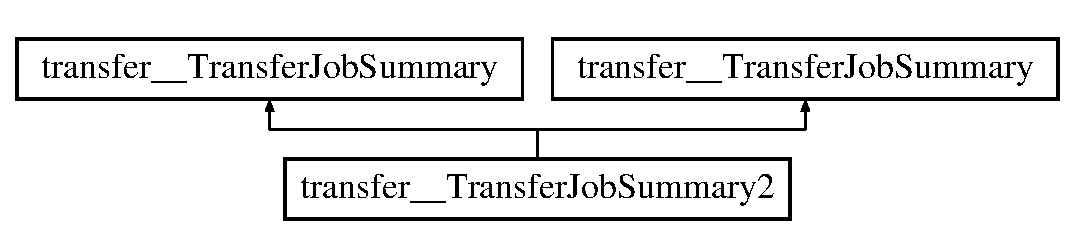
\includegraphics[height=2.000000cm]{classtransfer____TransferJobSummary2}
\end{center}
\end{figure}
\subsection*{Public Member Functions}
\begin{DoxyCompactItemize}
\item 
virtual int {\bfseries soap\_\-type} () const \label{classtransfer____TransferJobSummary2_a49fed8a5c2e528f712e6c79263827170}

\item 
virtual void {\bfseries soap\_\-default} (struct {\bf soap} $\ast$)\label{classtransfer____TransferJobSummary2_a72cd54a087b7b88cf29268d37cc4351a}

\item 
virtual void {\bfseries soap\_\-serialize} (struct {\bf soap} $\ast$) const \label{classtransfer____TransferJobSummary2_a16d105f097e289f0a2ffad0013f55e85}

\item 
virtual int {\bfseries soap\_\-put} (struct {\bf soap} $\ast$, const char $\ast$, const char $\ast$) const \label{classtransfer____TransferJobSummary2_a52cc4a67bae2c23aeba245c5f62053a4}

\item 
virtual int {\bfseries soap\_\-out} (struct {\bf soap} $\ast$, const char $\ast$, int, const char $\ast$) const \label{classtransfer____TransferJobSummary2_a03e68b7ccd108bebaeded8fd75fc46df}

\item 
virtual void $\ast$ {\bfseries soap\_\-get} (struct {\bf soap} $\ast$, const char $\ast$, const char $\ast$)\label{classtransfer____TransferJobSummary2_af5072c98bbd3ebe782aa21efc89aff04}

\item 
virtual void $\ast$ {\bfseries soap\_\-in} (struct {\bf soap} $\ast$, const char $\ast$, const char $\ast$)\label{classtransfer____TransferJobSummary2_a206be7a9d90b967f7b9e2b42419fdf9b}

\end{DoxyCompactItemize}
\subsection*{Data Fields}
\begin{DoxyCompactItemize}
\item 
int {\bf numReady}
\begin{DoxyCompactList}\small\item\em Element numReady of type xs:int. \item\end{DoxyCompactList}\item 
int {\bf numFinishing}
\begin{DoxyCompactList}\small\item\em Element numFinishing of type xs:int. \item\end{DoxyCompactList}\item 
int {\bf numAwaitingPrestage}
\begin{DoxyCompactList}\small\item\em Element numAwaitingPrestage of type xs:int. \item\end{DoxyCompactList}\item 
int {\bf numPrestaging}
\begin{DoxyCompactList}\small\item\em Element numPrestaging of type xs:int. \item\end{DoxyCompactList}\item 
int {\bf numWaitingCatalogRegistration}
\begin{DoxyCompactList}\small\item\em Element numWaitingCatalogRegistration of type xs:int. \item\end{DoxyCompactList}\item 
int {\bf numWaitingCatalogResolution}
\begin{DoxyCompactList}\small\item\em Element numWaitingCatalogResolution of type xs:int. \item\end{DoxyCompactList}\item 
int {\bf numWaitingPrestage}
\begin{DoxyCompactList}\small\item\em Element numWaitingPrestage of type xs:int. \item\end{DoxyCompactList}\end{DoxyCompactItemize}


\subsection{Detailed Description}
\char`\"{}http://transfer.data.glite.org\char`\"{}:TransferJobSummary2 is a complexType with complexContent extension of \char`\"{}http://transfer.data.glite.org\char`\"{}:TransferJobSummary. 

Definition at line 453 of file fts3-\/transfer-\/submit.h.



\subsection{Field Documentation}
\index{transfer\_\-\_\-TransferJobSummary2@{transfer\_\-\_\-TransferJobSummary2}!numAwaitingPrestage@{numAwaitingPrestage}}
\index{numAwaitingPrestage@{numAwaitingPrestage}!transfer__TransferJobSummary2@{transfer\_\-\_\-TransferJobSummary2}}
\subsubsection[{numAwaitingPrestage}]{\setlength{\rightskip}{0pt plus 5cm}int {\bf transfer\_\-\_\-TransferJobSummary2::numAwaitingPrestage}}\label{classtransfer____TransferJobSummary2_a911d1b53f9f080a54792c9103492795e}


Element numAwaitingPrestage of type xs:int. 

Required element. 

Definition at line 488 of file fts3-\/transfer-\/submit.h.

\index{transfer\_\-\_\-TransferJobSummary2@{transfer\_\-\_\-TransferJobSummary2}!numFinishing@{numFinishing}}
\index{numFinishing@{numFinishing}!transfer__TransferJobSummary2@{transfer\_\-\_\-TransferJobSummary2}}
\subsubsection[{numFinishing}]{\setlength{\rightskip}{0pt plus 5cm}int {\bf transfer\_\-\_\-TransferJobSummary2::numFinishing}}\label{classtransfer____TransferJobSummary2_a2f5afff6855a4741e7f124c80f367776}


Element numFinishing of type xs:int. 

Required element. 

Definition at line 486 of file fts3-\/transfer-\/submit.h.

\index{transfer\_\-\_\-TransferJobSummary2@{transfer\_\-\_\-TransferJobSummary2}!numPrestaging@{numPrestaging}}
\index{numPrestaging@{numPrestaging}!transfer__TransferJobSummary2@{transfer\_\-\_\-TransferJobSummary2}}
\subsubsection[{numPrestaging}]{\setlength{\rightskip}{0pt plus 5cm}int {\bf transfer\_\-\_\-TransferJobSummary2::numPrestaging}}\label{classtransfer____TransferJobSummary2_a0a6d0211253302a7e9f21f78433ecdd4}


Element numPrestaging of type xs:int. 

Required element. 

Definition at line 490 of file fts3-\/transfer-\/submit.h.

\index{transfer\_\-\_\-TransferJobSummary2@{transfer\_\-\_\-TransferJobSummary2}!numReady@{numReady}}
\index{numReady@{numReady}!transfer__TransferJobSummary2@{transfer\_\-\_\-TransferJobSummary2}}
\subsubsection[{numReady}]{\setlength{\rightskip}{0pt plus 5cm}int {\bf transfer\_\-\_\-TransferJobSummary2::numReady}}\label{classtransfer____TransferJobSummary2_a63dfdbbd95856fb3de0dbb1f9360d269}


Element numReady of type xs:int. 

Required element. 

Definition at line 484 of file fts3-\/transfer-\/submit.h.

\index{transfer\_\-\_\-TransferJobSummary2@{transfer\_\-\_\-TransferJobSummary2}!numWaitingCatalogRegistration@{numWaitingCatalogRegistration}}
\index{numWaitingCatalogRegistration@{numWaitingCatalogRegistration}!transfer__TransferJobSummary2@{transfer\_\-\_\-TransferJobSummary2}}
\subsubsection[{numWaitingCatalogRegistration}]{\setlength{\rightskip}{0pt plus 5cm}int {\bf transfer\_\-\_\-TransferJobSummary2::numWaitingCatalogRegistration}}\label{classtransfer____TransferJobSummary2_a235738ea2a4b73483420a8969571f709}


Element numWaitingCatalogRegistration of type xs:int. 

Required element. 

Definition at line 492 of file fts3-\/transfer-\/submit.h.

\index{transfer\_\-\_\-TransferJobSummary2@{transfer\_\-\_\-TransferJobSummary2}!numWaitingCatalogResolution@{numWaitingCatalogResolution}}
\index{numWaitingCatalogResolution@{numWaitingCatalogResolution}!transfer__TransferJobSummary2@{transfer\_\-\_\-TransferJobSummary2}}
\subsubsection[{numWaitingCatalogResolution}]{\setlength{\rightskip}{0pt plus 5cm}int {\bf transfer\_\-\_\-TransferJobSummary2::numWaitingCatalogResolution}}\label{classtransfer____TransferJobSummary2_af66bc9b0ee756f19dfbad94feeebbc80}


Element numWaitingCatalogResolution of type xs:int. 

Required element. 

Definition at line 494 of file fts3-\/transfer-\/submit.h.

\index{transfer\_\-\_\-TransferJobSummary2@{transfer\_\-\_\-TransferJobSummary2}!numWaitingPrestage@{numWaitingPrestage}}
\index{numWaitingPrestage@{numWaitingPrestage}!transfer__TransferJobSummary2@{transfer\_\-\_\-TransferJobSummary2}}
\subsubsection[{numWaitingPrestage}]{\setlength{\rightskip}{0pt plus 5cm}int {\bf transfer\_\-\_\-TransferJobSummary2::numWaitingPrestage}}\label{classtransfer____TransferJobSummary2_a883772b27795f6adc7d1551d26cc05f6}


Element numWaitingPrestage of type xs:int. 

Required element. 

Definition at line 496 of file fts3-\/transfer-\/submit.h.



The documentation for this class was generated from the following files:\begin{DoxyCompactItemize}
\item 
src/CLI/fts3-\/transfer-\/submit.h\item 
src/CLI/ftsStub.h\item 
src/CLI/ftsC.cpp\end{DoxyCompactItemize}

\section{transfer\_\-\_\-TransferParams Class Reference}
\label{classtransfer____TransferParams}\index{transfer\_\-\_\-TransferParams@{transfer\_\-\_\-TransferParams}}


\char`\"{}http://transfer.data.glite.org\char`\"{}:TransferParams is a complexType.  




{\ttfamily \#include $<$fts3-\/transfer-\/submit.h$>$}

\subsection*{Public Member Functions}
\begin{DoxyCompactItemize}
\item 
virtual int {\bfseries soap\_\-type} () const \label{classtransfer____TransferParams_acca6acc764bd1fe03ef2aefdce8b2e6c}

\item 
virtual void {\bfseries soap\_\-default} (struct {\bf soap} $\ast$)\label{classtransfer____TransferParams_aa85cbcf0c2d7405ef86e9fcbb5e975c4}

\item 
virtual void {\bfseries soap\_\-serialize} (struct {\bf soap} $\ast$) const \label{classtransfer____TransferParams_afb6351523ca0b245c6a085215bd2a15e}

\item 
virtual int {\bfseries soap\_\-put} (struct {\bf soap} $\ast$, const char $\ast$, const char $\ast$) const \label{classtransfer____TransferParams_a9d494d69d5fc18e6641f6bbae96a6cc0}

\item 
virtual int {\bfseries soap\_\-out} (struct {\bf soap} $\ast$, const char $\ast$, int, const char $\ast$) const \label{classtransfer____TransferParams_a18ada0a242ed2166baddfe4967c7c1a2}

\item 
virtual void $\ast$ {\bfseries soap\_\-get} (struct {\bf soap} $\ast$, const char $\ast$, const char $\ast$)\label{classtransfer____TransferParams_a9bd36bdebda7b93d15cf35543d80aaea}

\item 
virtual void $\ast$ {\bfseries soap\_\-in} (struct {\bf soap} $\ast$, const char $\ast$, const char $\ast$)\label{classtransfer____TransferParams_ac7645705dda8399a38e8019adcd3f29d}

\end{DoxyCompactItemize}
\subsection*{Data Fields}
\begin{DoxyCompactItemize}
\item 
std::vector$<$ std::string $>$ {\bf keys}
\begin{DoxyCompactList}\small\item\em Vector of std::string with length 1..unbounded. \item\end{DoxyCompactList}\item 
std::vector$<$ std::string $>$ {\bf values}
\begin{DoxyCompactList}\small\item\em Vector of std::string with length 1..unbounded. \item\end{DoxyCompactList}\item 
struct {\bf soap} $\ast$ {\bf soap}\label{classtransfer____TransferParams_a9ea0e57bdb9dc72a1f329eef83e32547}

\begin{DoxyCompactList}\small\item\em A handle to the soap struct that manages this instance (automatically set) \item\end{DoxyCompactList}\end{DoxyCompactItemize}


\subsection{Detailed Description}
\char`\"{}http://transfer.data.glite.org\char`\"{}:TransferParams is a complexType. 

Definition at line 153 of file fts3-\/transfer-\/submit.h.



\subsection{Field Documentation}
\index{transfer\_\-\_\-TransferParams@{transfer\_\-\_\-TransferParams}!keys@{keys}}
\index{keys@{keys}!transfer__TransferParams@{transfer\_\-\_\-TransferParams}}
\subsubsection[{keys}]{\setlength{\rightskip}{0pt plus 5cm}std::vector$<$ std::string $>$ {\bf transfer\_\-\_\-TransferParams::keys}}\label{classtransfer____TransferParams_a141364cc99cab03aab48e642905bcac5}


Vector of std::string with length 1..unbounded. 

Nullable pointer. 

Definition at line 156 of file fts3-\/transfer-\/submit.h.

\index{transfer\_\-\_\-TransferParams@{transfer\_\-\_\-TransferParams}!values@{values}}
\index{values@{values}!transfer__TransferParams@{transfer\_\-\_\-TransferParams}}
\subsubsection[{values}]{\setlength{\rightskip}{0pt plus 5cm}std::vector$<$ std::string $>$ {\bf transfer\_\-\_\-TransferParams::values}}\label{classtransfer____TransferParams_a66e689a5a75be59fb3025c3681983930}


Vector of std::string with length 1..unbounded. 

Nullable pointer. 

Definition at line 158 of file fts3-\/transfer-\/submit.h.



The documentation for this class was generated from the following files:\begin{DoxyCompactItemize}
\item 
src/CLI/fts3-\/transfer-\/submit.h\item 
src/CLI/ftsStub.h\item 
src/CLI/ftsC.cpp\end{DoxyCompactItemize}

\printindex
\end{document}
